% **************************************************
% Document Class Definition
% **************************************************
\documentclass[%
	paper=A4,					% paper size --> A4 is default in Germany
	twoside=true,				% onesite or twoside printing
	openright,					% doublepage cleaning ends up right side
	parskip=full,				% spacing value / method for paragraphs
	chapterprefix=true,			% prefix for chapter marks
	11pt,						% font size
	headings=normal,			% size of headings
	bibliography=totoc,			% include bib in toc
	listof=totoc,				% include listof entries in toc
	titlepage=on,				% own page for each title page
	captions=tableabove,		% display table captions above the float env
	draft=false,				% value for draft version
]{scrreprt}%

% **************************************************
% Debug LaTeX Information
% **************************************************
%\listfiles

% **************************************************
% Information and Commands for Reuse
% **************************************************
\newcommand{\thesisTitle}{Search of the \dst dibaryon at the LHC with the ALICE Experiment}
\newcommand{\thesisName}{Pietro Fecchio}
\newcommand{\thesisSubject}{Laurea Magistrale in Fisica}
\newcommand{\thesisDate}{August 19, 2018}
\newcommand{\thesisVersion}{First Draft}

\newcommand{\thesisReviewer}{Prof. Stefano Spataro}
\newcommand{\thesisReviewerUniversity}{\protect{Universit\`a degli Studi di Torino}}
\newcommand{\thesisReviewerDepartment}{I.N.F.N. Torino}

\newcommand{\thesisFirstSupervisor}{Prof. Massimo Masera}
\newcommand{\thesisFirstSupervisorUniversity}{\protect{Universit\`a degli Studi di Torino}}
\newcommand{\thesisFirstSupervisorDepartment}{I.N.F.N. Torino}

\newcommand{\thesisSecondSupervisor}{Prof. Stefania Bufalino}
\newcommand{\thesisSecondSupervisorUniversity}{\protect{Universit\`a degli Studi di Torino}}
\newcommand{\thesisSecondSupervisorDepartment}{I.N.F.N. Torino}

\newcommand{\thesisUniversity}{\protect{Universit\`a degli Studi di Torino}}
\newcommand{\thesisUniversityDepartment}{Dipartimento di Fisica}
\newcommand{\thesisUniversityInstitute}{Scuola di Scienze della Natura}
\newcommand{\thesisUniversityStreetAddress}{Via P.Giuria, 1 - 10125 Torino}
\newcommand{\thesisUniversityCity}{Torino}

% **************************************************
% Package for Custom COMMAND

\usepackage{xspace}
\usepackage{lineno}
\usepackage{feynmp-auto}
\usepackage{amsmath}
\usepackage{amssymb}
\usepackage{relsize}
\usepackage{tabularx}
\usepackage{booktabs}

% **************************************************
% Custom COMMAND
% **************************************************
\newcommand{\s}      {\ensuremath{\sqrt{s}}\xspace}
\newcommand{\sotev}  {\ensuremath{\sqrt{s}} = 8 TeV\xspace}
\newcommand{\sctev}  {\ensuremath{\sqrt{s_{NN}}} = 5.02 TeV\xspace}
\newcommand{\sdtev}  {\ensuremath{\sqrt{s_{NN}}} = 2.76 TeV\xspace}
\newcommand{\trtev}  {\ensuremath{\sqrt{s}} = 13 TeV\xspace} % da controllare che sia giusto

\newcommand{\pt}    {\ensuremath{p_{\mathrm{T}}}\xspace}
\newcommand{\pti}   {\ensuremath{p_{\mathrm{T},i}}\xspace}

\newcommand{\pip}       {\ensuremath{\pi^{+}}\xspace}
\newcommand{\pim}       {\ensuremath{\pi^{-}}\xspace}
\newcommand{\ds}        {\ensuremath{d^*}\xspace}
\newcommand{\dst}       {\ensuremath{{d}^{*}(2380)}\xspace}
\newcommand{\dstdecay}  {\ensuremath{{d}^{*}(2380) \rightarrow {d}\ +\pi^{+}+ \pi^{-}}\xspace} % controllare che gli spazi vadano bene
% \newcommand{\dstdecayc}{\ensuremath{{d}^{*}(2380) \rightarrow {d}\pi^{+}\pi^{-}}\xspace}
\newcommand{\dpp}    {\ensuremath{{d} + \pi^{+}+ \pi^{-}}\xspace}
\newcommand{\minv}   {M\ensuremath{_{{d} \pi \pi}}\xspace}
\newcommand{\mpp}    {M\ensuremath{_{\pi \pi}}\xspace}
\newcommand{\Tch}    {\ensuremath{T_{\mathrm{ch}}}\xspace}
\newcommand{\PbPb}   {Pb--Pb\xspace}
\newcommand{\pPb}    {p--Pb\xspace}

\newcommand{\mevc}   {\mbox{\ensuremath{\mathrm{MeV}/c}}\xspace}
\newcommand{\gevc}   {\mbox{\ensuremath{\mathrm{GeV}/c}}\xspace}
\newcommand{\mevcs}  {\mbox{\ensuremath{\mathrm{MeV}/c^{2}}}\xspace}
\newcommand{\gevcs}  {\mbox{\ensuremath{\mathrm{GeV}/c^{2}}}\xspace}

\newcommand{\dedx}{\ensuremath{\mathrm{d}\hspace{-0.1em}E/\mathrm{d}x}\xspace}

\newcommand{\Lagr}{\mathcal{L}}
\newcommand{\boldm}[1] {\mathversion{bold}#1\mathversion{normal}}

\DeclareMathOperator{\Tr}{Tr}

% **************************************************
% Load and Configure Packages
% **************************************************
\usepackage[utf8]{inputenc}		% defines file's character encoding
\usepackage[english]{babel}		% babel system, adjust the language of the content

\usepackage[					% clean thesis style
	figuresep=colon,%
	sansserif=false,%
	hangfigurecaption=false,%
	hangsection=true,%
	hangsubsection=true,%
	colorize=full,%
	colortheme=bluemagenta,%
	bibsys=bibtex,%
	bibfile=bib-refs,%
	bibstyle=numeric,%
]{cleanthesis}

\hypersetup{					% setup the hyperref-package options
	pdftitle={\thesisTitle},	% 	- title (PDF meta)
	pdfsubject={\thesisSubject},% 	- subject (PDF meta)
	pdfauthor={\thesisName},	% 	- author (PDF meta)
	plainpages=false,			% 	-
	colorlinks=false,			% 	- colorize links?
	pdfborder={0 0 0},			% 	-
	breaklinks=true,			% 	- allow line break inside links
	bookmarksnumbered=true,		%
	bookmarksopen=true			%
}

% **************************************************
% Document CONTENT
% **************************************************
\begin{document}

% --------------------------
% rename document parts
% --------------------------
\renewcaptionname{english}{\figurename}{Fig.}
\renewcaptionname{english}{\tablename}{Tab.}

% --------------------------
% Front matter
% --------------------------
\pagenumbering{roman}			% roman page numbing (invisible for empty page style)
\pagestyle{empty}				% no header or footers
% % !TEX root = ../tesi.tex
%
% ------------------------------------  --> cover title page
\begin{titlepage}
	\pdfbookmark[0]{Cover}{Cover}
	\flushright
	\hfill
	\vfill
	{\LARGE\thesisTitle \par}
	\rule[5pt]{\textwidth}{.4pt} \par
	{\Large\thesisName}
	\vfill
	\textit{\large\thesisDate}
\end{titlepage}


% ------------------------------------  --> main title page
\begin{titlepage}
	\pdfbookmark[0]{Titlepage}{Titlepage}
	\tgherosfont
	\centering

	{\Large \thesisUniversity} \\[4mm]
	
\includegraphics[width=4.5cm]{gfx/logo} \\[2mm]
	\textsf{\large \thesisUniversityInstitute} \\
	\textsf{\large \thesisUniversityDepartment} \\

	\vfill
	{\large \thesisSubject} \\[5mm]
	{\LARGE \color{ctcolortitle}\textbf{\thesisTitle} \\[10mm]}
	{\Large \thesisName} \\

	\vfill
	\begin{minipage}[t]{.27\textwidth}
		\raggedleft
		\textit{Reviewer}
	\end{minipage}
	\hspace*{15pt}
	\begin{minipage}[t]{.65\textwidth}
		{\large \thesisReviewer}
	  	% {\small \thesisReviewerDepartment} \\[-1mm]
		% {\small \thesisReviewerUniversity}
	\end{minipage} \\[10mm]
	\begin{minipage}[t]{.27\textwidth}
		\raggedleft
		\textit{Supervisor}
	\end{minipage}
	\hspace*{15pt}
	\begin{minipage}[t]{.65\textwidth}
		{\large \thesisFirstSupervisor} 
		% {\small \thesisFirstSupervisorUniversity} \\[-1mm]
	  	% {\small \thesisFirstSupervisorDepartment} 
	\end{minipage} \\[5mm]
	\begin{minipage}[t]{.27\textwidth}
		\raggedleft
		\textit{Co-supervisor}
	\end{minipage}
	\hspace*{15pt}
	\begin{minipage}[t]{.65\textwidth}
		{\large \thesisSecondSupervisor}
		% {\small \thesisSecondSupervisorUniversity} \\[-1mm]
	  	% {\small \thesisSecondSupervisorDepartment} 
	\end{minipage} \\[10mm]

	\thesisDate \\

\end{titlepage}


% ------------------------------------  --> lower title back for single page layout
\hfill
\vfill
{
	\small
	\textbf{\thesisName} \\
	\textit{\thesisTitle} \\
	\thesisSubject, \thesisDate \\
	Reviewer: \thesisReviewer\  \\
	Supervisors: \thesisFirstSupervisor\ and \thesisSecondSupervisor \\[1.5em]
	\textbf{\thesisUniversity} \\
	\thesisUniversityInstitute \\
	\thesisUniversityDepartment \\
	\thesisUniversityStreetAddress
}
		% INCLUDE: all titlepages
% \cleardoublepage

\pagestyle{plain}				% display just page numbers
% % !TEX root = ../thesis-example.tex
%
\pdfbookmark[0]{Abstract}{Abstract}
\chapter*{Abstract}
\label{sec:abstract}
\vspace*{-10mm}

\blindtext
		% INCLUDE: the abstracts (english and german)
% \cleardoublepage
%
% % !TEX root = ../thesis-example.tex
%
\pdfbookmark[0]{Acknowledgement}{Acknowledgement}
\chapter*{Acknowledgement}
\label{sec:acknowledgement}
\vspace*{-10mm}

\Blindtext[2][2]
 % INCLUDE: acknowledgement
% \cleardoublepage
%
% \setcounter{tocdepth}{2}		% define depth of toc
% \tableofcontents				% display table of contents
% \cleardoublepage

% --------------------------
% Body matter
% --------------------------
\pagenumbering{arabic}			% arabic page numbering
\setcounter{page}{1}			% set page counter
\pagestyle{maincontentstyle} 	% fancy header and footer

% % !TEX root = ../main.tex
%
\chapter{High Energy Nuclear Physics}
\label{sec:1}

\cleanchapterquote{Three quarks for Muster Mark! \\
                   Sure he has not got much of a bark\\
                   And sure any he has it's all beside the mark.}{James Joyce}{(Finnegans Wake)}

According to cosmological theories, in its early stages the Universe was extremely hot and dense.
In the first few microseconds, the energy densisty was so high that hadrons could not be formed and
their foundamental constituents were in a deconfined state. When the energy density has decreased
enough, a phase transition led to the formation of the ordinary matter. 

High Energy Nuclear Physics (HENP) investigates the hot and dense nuclear matter and the properties
of its phase transition into ordinary matter through the study of ultra-relativistic heavy-ion collisions. 
The aim is to improve our understandig of the behaviour of the matter in extereme conditions and of the
Universe at the beginning of its life.

\section{QCD: the theory of the Strong Interaction}
\label{sec:1.1}

In 1964 M. Gell-Mann and G. Zweig proposed independently a model that could explain the existence of
the great variety of hadrons discovered in the 1950s and 1960s 
\cite{gellmann, zweig1, zweig2}. 
This model, known as the Static Quark Model, was based on the assumption that hadrons are not
fundamental particles, but they are composed states of elementary constituents called quarks.
In this way it was possible to explain the large number of particles observed and their properties,
which showed some sort of pattern, in term of constituents properties.
Furthermore, thanks to the Static Quark Model, it was possible predict new hadrons (e.g. 
$\Omega^{-}\xspace$) and to explain why certain particles don't exist (e.g. baryons with $S=+1$).
However, this model could not deal with many questions: why there is no evidence of free quarks?
What hold quarks together in a hadron? Why the $\Delta^{++}$ baryon exists despite is forbidden
by Pauli's Principle?
In order to answer these questions it was necessary to introduce a new quantum number the colour
\cite{fritzsch-gellmann}. The introduction of the colour led to the formulation of a quantum field theory
for the Strong Interaction, inspired by the Quantum Electrodynamics (QED), the Quantum Chromodynamics
(QCD).

The QCD is a non-Abelian quantum gauge theory, based on the invariance under local $\mathrm{SU(3)}_{c}$ 
group transformations. The choice of this particular symmetry group is due to the hypothesis
that the colour comes in three different states: red, blue and green.
The local invariance under $\mathrm{SU(3)}_{c}$ implies the existence of 8 massless gauge bosons
mediators of the colour interaction, called gluons \cite{fr-gm-hl-gluons}.
Therefore the QCD Lagrangian can be written as:
\begin{equation}
    \Lagr_{\mathrm{QCD}} = \bar{\psi_{i}}(i(\gamma^{\mu}D_{\mu})_{ij}-m\,\delta_{ij})\psi_{j} 
    - \frac{1}{4}G^{a}_{\mu \nu} G^{\mu \nu}_{a}
\end{equation}
where the first term is related to quarks fields while the second is releted to gluons fields.
In the first term $\psi_{i}(x)$ represents the quarks fields expressed in the fundamental 
representation of $\mathrm{SU(3)}_{c}$, while $D_{\mu}$ is the covariant derivative, defined as:
\begin{equation}
    D_{\mu} = \partial_{\mu} - ig_{s}A^{a}_{\mu}\lambda_{a}.
\end{equation}
In this derivarives shows up the coupling constant for the Strong Interaction $g_{s}$, the 
Gell-Mann matrices $\lambda_{\alpha}$ which gives a representation of the generators of 
$\mathrm{SU(3)}_{c}$ symmetry group, and the gluon field $A(x)$.
This first term of the QCD Lagrangian represents the quarks-gluons interaction via a 
QED-like vertex.

\vspace{1cm}
\begin{figure}[!h]
\captionsetup{justification=centering}
\centering
    \begin{fmffile}{2gluoni1quark}
        \begin{fmfgraph*}(80,60)
            \fmfleft{i1}
            \fmfright{o1,o2}
            \fmf{gluon}{i1,v1}
            \fmf{fermion}{o1,v1,o2}
            \fmflabel{$a$}{i1}
            \fmflabel{$\psi_i$}{o1}
            \fmflabel{$\psi_j$}{o2}
        \end{fmfgraph*}
    \end{fmffile}
\vspace{1cm}
\caption{Feynman diagram for the gluon-quarks interaction.}
\end{figure}

The second term of the Lagrangian $G^{a}_{\mu \nu}$ represents the gauge invariant gluon field 
strength tensor, and can be written as:
\begin{equation}
    G^{a}_{\mu \nu} = \partial_{\mu} A^{a}_{\nu} - \partial_{\nu} A^{a}_{\mu} + 
    g_{s} f^{abc} A^{b}_{\mu} A^{c}_{\nu}.
\end{equation}
In this tensor $g_{s} f^{abc} A^{b}_{\mu} A^{c}_{\nu}\ $ is the non-Abelian part of the theory, 
which implies the self-interactions among gluons. This interactions have resulted from the
fact that gluons carry a colour and an anti-colour charge, so they can interact among themselves.
Therefore in addition to the QED-like vertex, in the QCD, 3 gluons and 4 gluons vertex are allowed
at the tree level. 
The existence of the gluons vertex allows to have gluons loops.

\vspace{1cm}
\begin{figure}[!h]
    \hspace{2cm}
    \begin{fmffile}{3gluoni}
        \begin{fmfgraph*}(80,60)
            \fmfleft{i1}
            \fmfright{o1,o2}
            \fmf{gluon}{i1,v1}
            \fmf{gluon}{o1,v1,o2}
            \fmflabel{$a,\mu$}{i1}
            \fmflabel{$b,\nu$}{o1}
            \fmflabel{$c,\rho$}{o2}
        \end{fmfgraph*}
    \end{fmffile}

    \vspace{-2.1cm}
    \hspace{8cm}
    \begin{fmffile}{4gluoni}
        \begin{fmfgraph*}(80,60)
            \fmfleft{i1,i2}
            \fmfright{o1,o2}
            \fmf{gluon}{i1,v1,i2}
            \fmf{gluon}{o1,v1,o2}
            \fmflabel{$a,\mu$}{i1}
            \fmflabel{$b,\nu$}{i2}
            \fmflabel{$c,\rho$}{o1}
            \fmflabel{$d,\sigma$}{o2}
        \end{fmfgraph*}
    \end{fmffile}
\vspace{1cm}
\caption{Feynman diagrams for the gluon-gluon interactions at the tree level.}
\end{figure}

In the renormalization process of the theory, the non-Abelian nature of the QCD brings to the 
so-called \textit{anti-screening} in colour interaction.
%, since gluons loops have to be considered.
%Indeed, 
Adding loop corrections to the gluons propagator, gluons loops contribute to the sum with
opposite sign respect to the quarks loops.
Therefore, in addition to the QED-like \textit{screening} effect, there is an 
\textit{anti-screening} effect due to gluons loops.
As a result, the QCD shows up its specific features, \textit{asymptotic freedom} and 
\textit{confinement}.

Setting $\alpha_{s} = g^{2}_{s}/4\pi\ $ strong coupling constant can be written as \cite{pdg}:
\begin{equation} \label{eq:alphastrong1}
    \alpha_{s}(Q^{2}) = \frac{\alpha_{s}(\mu^{2})}{1 + \alpha_{s}(\mu^{2})(33 - 2\,n_{f})
    \ln(Q^{2}/\mu^{2})}
\end{equation}
where $n_{f}\ $ is the number of quark families and $\mu\ $ is the renormalization scale of 
the theory.
For high transferred momenta $\alpha_{s}\ $ goes to zero and the QCD becomes a free theory and 
this regime is called \textit{asymptotic freedom}. At low $Q^{2}\ $ the Strong copuling diverges,
forcing quarks to be strongly bound in hadrons: the so-called \textit{confinement} regime. 
This behaviour of the QCD copuling constant has been confirmed by experimental results over the
years as shown in Figure \ref{fig:alpharun}.
The equation \ref{eq:alphastrong1} can be rewritten fixing the energy scale:
\begin{equation} \label{eq:alphastrong2}
    \alpha_{s}(Q^{2}) = \frac{12 \pi}{(33 - 2\,n_{f})\ln(Q^{2}/\Lambda_{\mathrm{QCD}})}
\end{equation}
where $\Lambda_{\mathrm{QCD}}$ is the renormalization scale of QCD (typically $\approx 200$ MeV).

\begin{figure}
    \captionsetup{justification=centering}
    \centering
    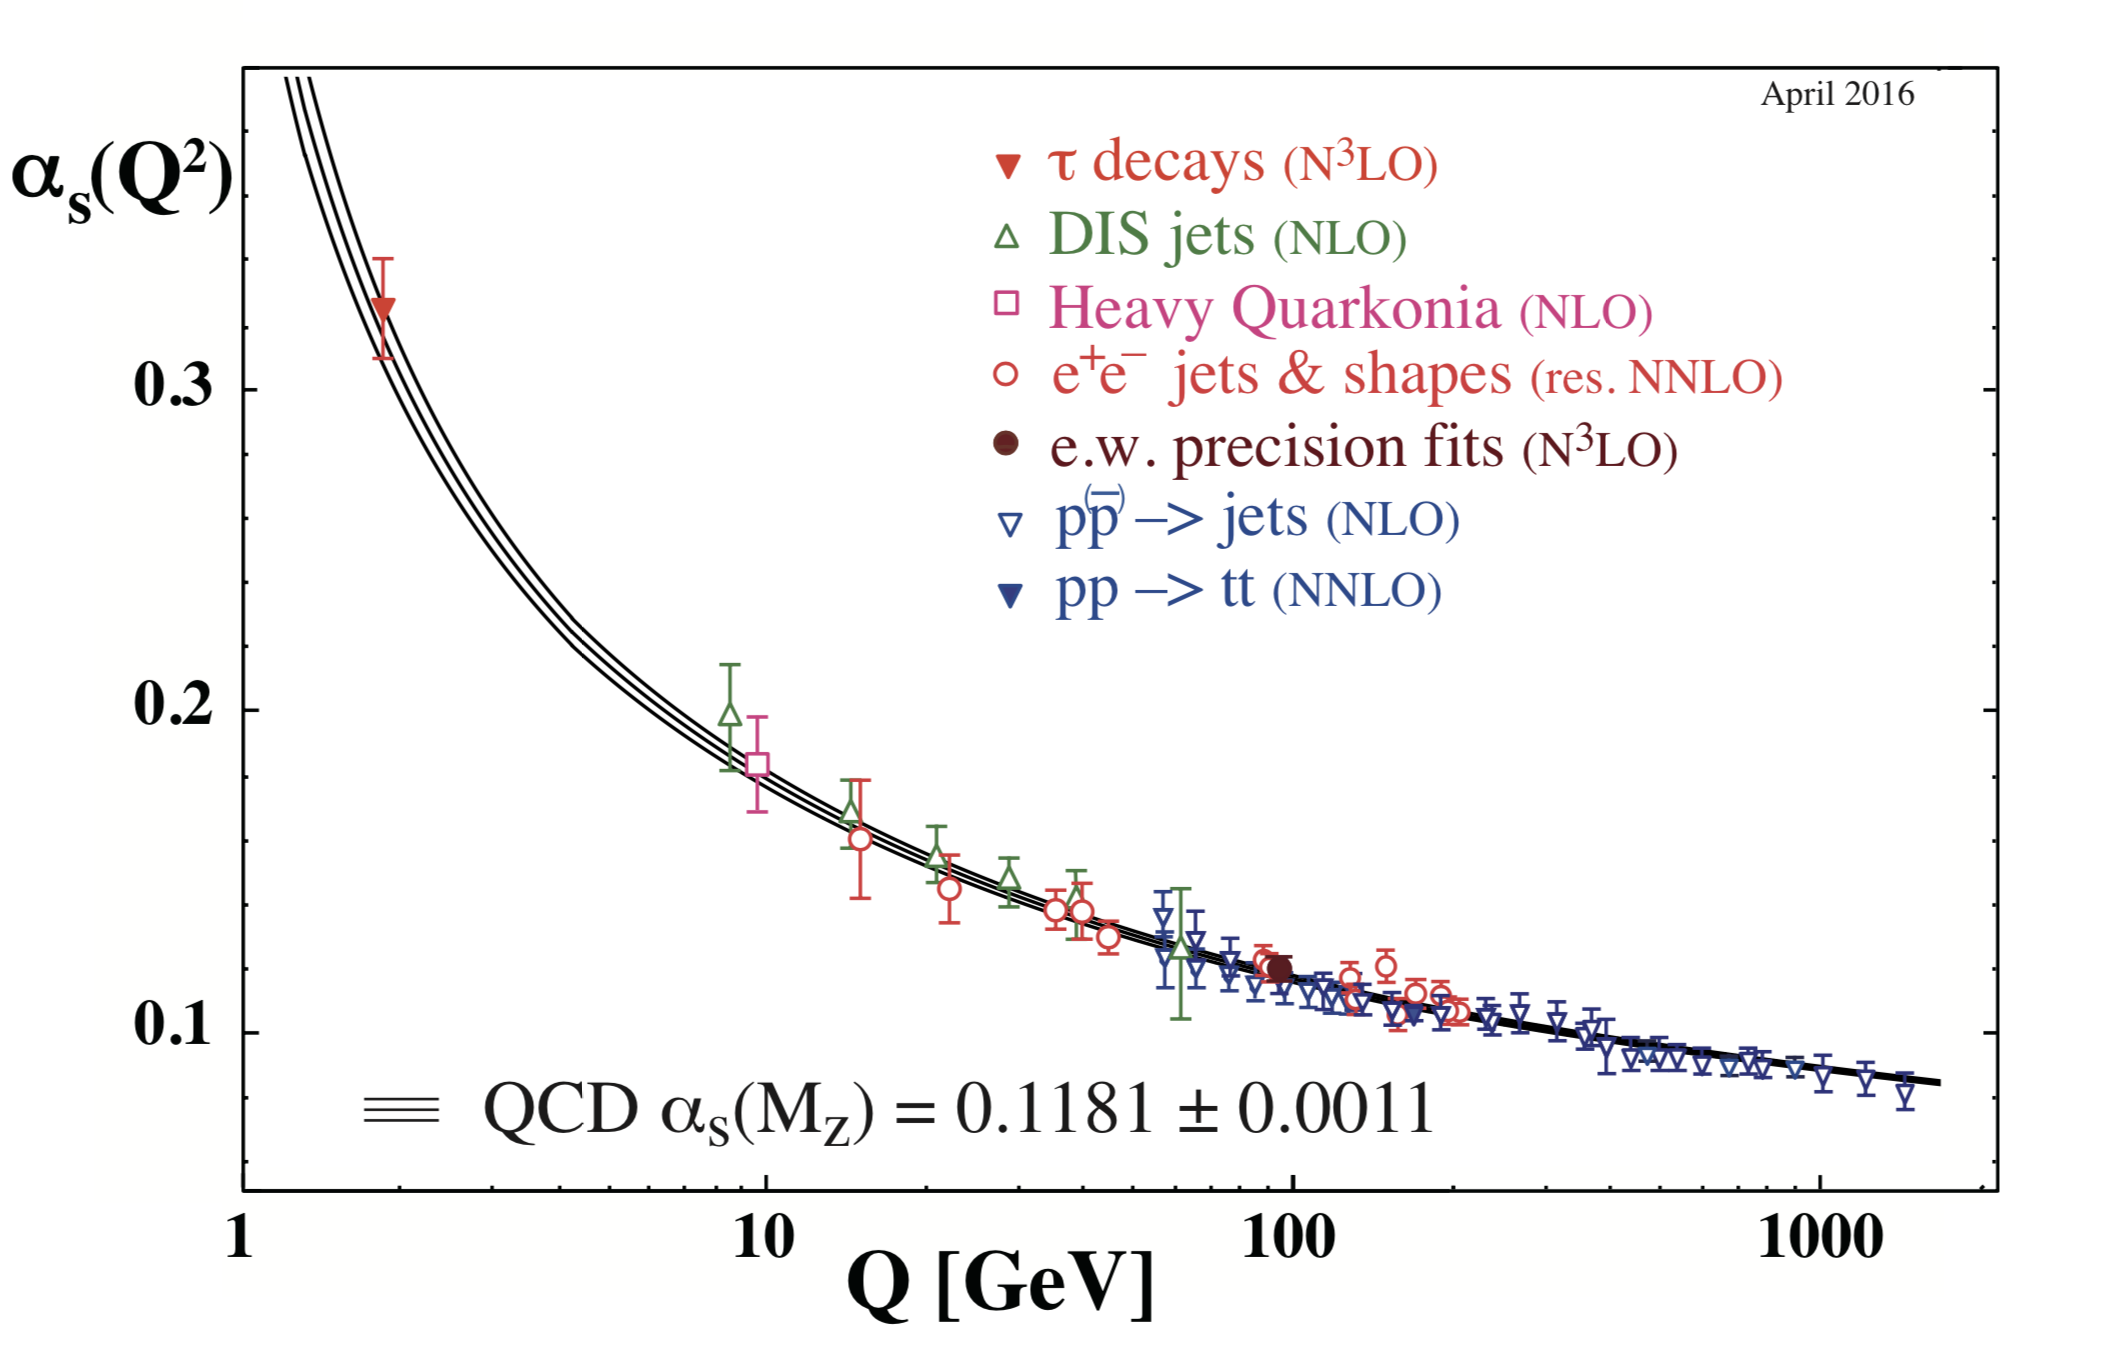
\includegraphics[width=0.8\textwidth]{gfx/alpharun}
	\caption{Summary of measurements of $\alpha_{s}$ as a function of the energy scale $Q$ \cite{pdg}.}
	\label{fig:alpharun}
\end{figure}

In QCD the perturbative approach used to calculate the elements of the scattering matrix (pQCD), is 
possible only for high $Q^{2}\ $ processes ($Q^{2} \gg \mu^{2}$, thus $\alpha_{s} \ll 1$).
As already mentioned, in low transferred momentum processes $\alpha_{s}$ diverges. 
Therefore, is impossible to express the elements of the scattering matrix in terms of power series
expansion of the Strong copuling constant.
In this regime it is still possible to evaluate the Green’s functions of the QCD Lagrangian
on a space-time lattice with spacing a, as proposed in 1974 by Wilson \cite{lattice}.
With this method, called lattice QCD (lQCD) is possible to extrapolate to the continuum 
($a \rightarrow 0$) and get results to be compared with the experiments.

%
%
\section{States of hadronic matter}
\label{sec:1.2}

One of the interesting consequences of the running copuling constant is the possibility of having
different states of the hadronic matter. The state is essentially determined by the mean transferred 
momentum in the interactions which define the value of $\alpha_{s}$. 
A system with low mean transferred momentum it is in the \textit{confinement} regime, therefore quarks
and gluons are required to be confined in hadrons. Otherwise in high mean transferred momentum systems,
the \textit{asymptotic freedom} regime allows the formation of a plasma where quarks and gluons are
essentially free. This state of matter is called Quark Gluon Plasma (QGP) and is supposed that the 
universe was in this state in the first microseconds after the Big Bang.
One of the main goals of the HENP is the study of the phase transitions between the different
states of the hadronic matter.

Considering a system with finite dimensions, composed by hadronic matter, can be useful to describe it 
using thermodinamical variables like temperature $(T)$ and chemical potential $(\mu)$. In this
specific framework the chemical potential is interpreted as the energy required to create a 
baryonic state and it is called baryon chemical potential $(\mu_{B})$. 
Figure \ref{fig:qgpdiagram} shows the phase diagram of the QCD matter predicted by the theory and 
the values of temperature $T$ and baryon chemical potential $(\mu_{B})$ which are accessible
experimentally in high energy heavy ion collisions.

\begin{figure}
    \centering
    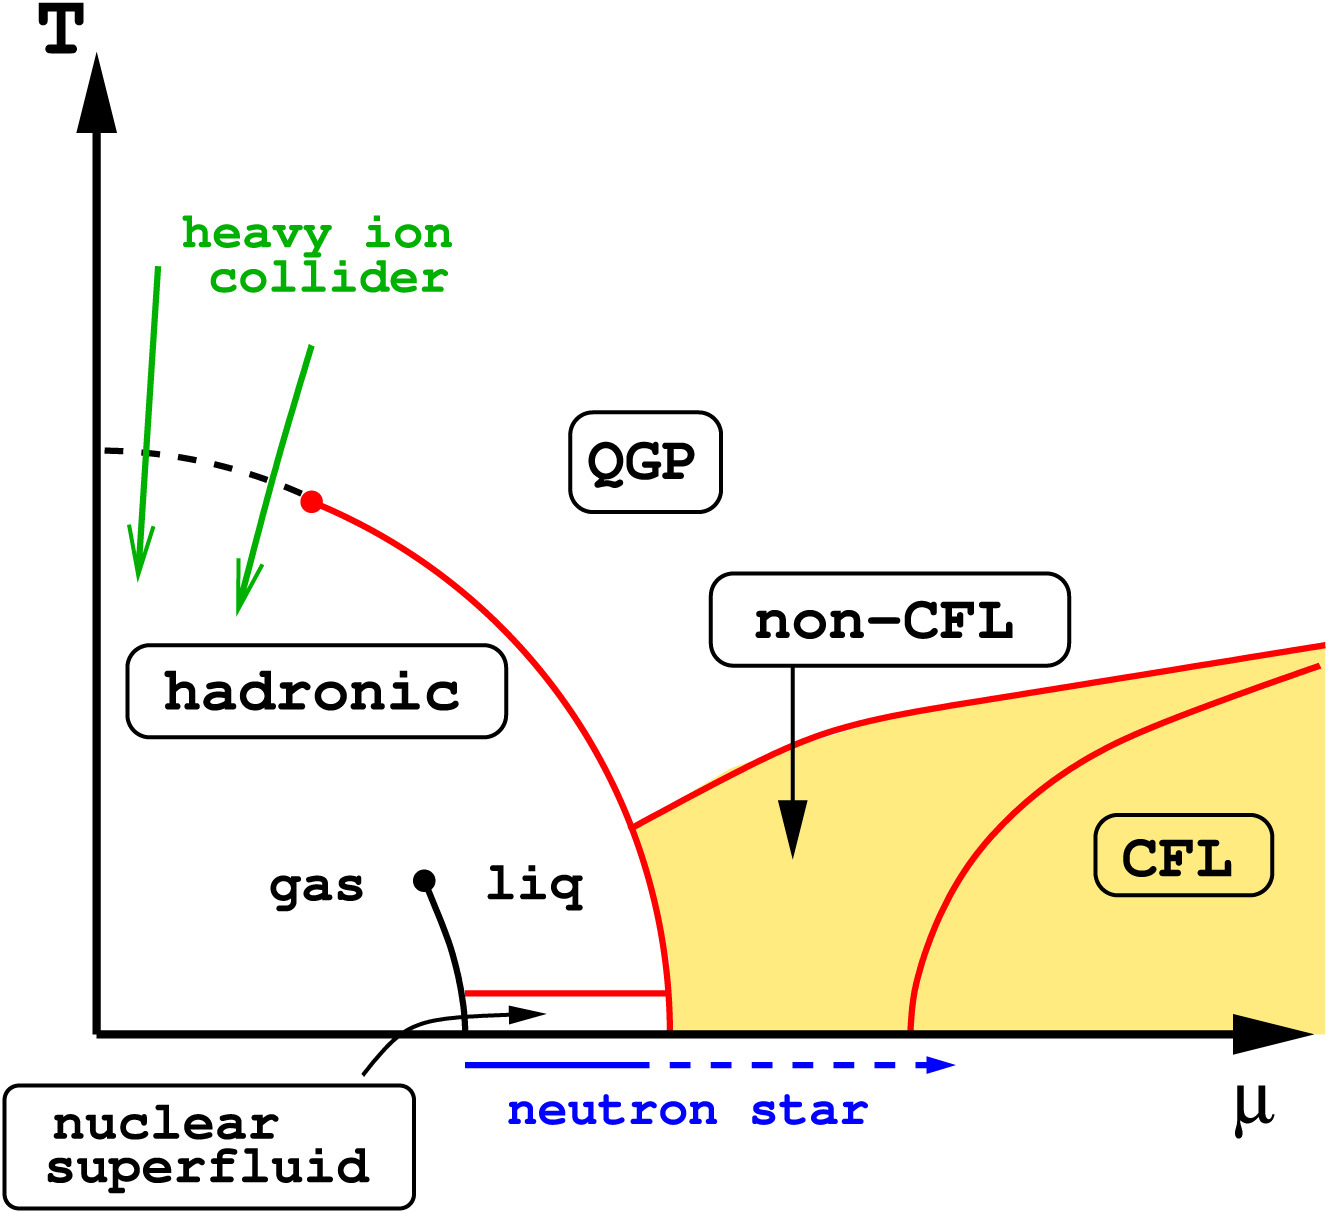
\includegraphics[width=0.6\textwidth]{gfx/qgpphase}
	\caption{Schematic representation of the nuclear matter phase diagram from \cite{qgpphase}. QGP refers to the Quark Gluon Plasma state, CFL (Colour-Flavour Locked) corresponds to the colour superconducting phase that is present in systems with high baryon chemical potential. The green arrows represent the phase space investigated by collider experiments at the Relativistic Heavy Ion Collider (RHIC) and at the LHC.}
	\label{fig:qgpdiagram}
\end{figure}

The origin of the diagram (T$=\mu_{B}=0$ GeV) corresponds to the QCD vacuum. At T$=0$ GeV, $\mu_{B}$ is 
the energy required to create a baryonic state, therefore ordinary matter (proton, neutrons and nuclei)
sits around $1$ GeV on the $\mu_{B}$ axis. Along the $\mu_{B}$ axis lies a phase transition to a state,
the Color Superconducting Phase, that has been hypothesised to be present in matter at high density,
e.g. in  the core of neutron stars \cite{csp}.
Along the T axis, where $\mu_{B}=0$, there is a phase transition when T$\ \gg \Lambda_{\mathrm{QCD}}$. 
At this temperatures the average momentum exchange between quarks and gluons is so high that they reach
the \textit{asymptotic freedom}, hence they are no longer confined in colour singlets states.
In these conditions they constitute a plasma of free coloured partons, similar to the primordial 
universe: the aforementioned QGP.

The order of the phase transition is determined by the behaviour of the derivatives of the free energy
of the system with respect to time. It basically describes how fast the free energy varies in a 
neighbourhood of the transition temperature.
A first order transitions takes place when a latent heat is present, leading to a discontinuous free
energy first derivatives and variation of entropy.
If no latent heat is involved in the process, occours a second order transition. The free energy 
first derivative is continuous, while derivatives of higher than first order of the free energy are 
discontinuous.
When the transition occours with a continuous behaviour of the free energy and its derivatives,
it is called a \textit{crossover} transition.
In $\mu_{B}=0$ conditions, the transition from hadron gas to the QGP takes place when T $\approx 150$ MeV
with a \textit{crossover} transition.

%
%
\section{Heavy Ion Collisions}
\label{sec:1.3}

The QCD phase diagram is derived by theories and models, but their predictions are difficult to test.
For the T $\approx0$ GeV and high $\mu_{B}$ region, important suggestions can come from astronomic observations 
of neutron stars. 
For high T regions, instead, the only known way to cross the phase boundary between ordinary hadronic matter
and QGP is by colliding ultrarelativistic heavy ions in the laboratory.

The journey of the High Energy Nuclear Physics started in the '70 at the Lawrence Berkeley National Laboratory
where the first experiments on heavy ions collisions (HIC) was performed at modestly relativistic conditions 
($\approx 2\ $ GeV/nucleon).
In 1986, two HIC experiments started simultaneously at the Super Proton Syncrotron (SPS) at CERN and at the
Alternate Gradient Syncrotron (AGS) at Brookhaven, colliding O ions at fixed target at higher energies.
Nowdays the two main hadron colliders active with an HIC program and dedicated experiments are the
Relativistic Heavy Ion Collider (RHIC) at the Brookhaven National Laboratory (BNL) and the Large Hadron
Collider (LHC) at CERN.

%
\subsection{The "Little Bang" at the LHC}
\label{sec:1.3.1}

Atomic nuclei are composite systems of nucleons with finite dimensions. When they collide at 
ultrarelativistic energies the problem of the description of the collision, that can be very
complex, arises.
The Glauber Model \cite{glauber} is a semi-classical model describing nucleus–nucleus 
interaction in terms of nucleon–nucleon (NN) interactions.
The Glauber Model is based on the assumption of the \textit{optical limit}:
\begin{itemize}
    \item nucleons are point like and independent inside the nuclei;
    \item only hadronic interactions are considered: protons and neutrons cannot be distinguished;
    \item the collision does not deflect colliding nucleons: they travel in a straight line;
    \item the cross section for an elementary nucleon-nucleon interaction is constant during the whole 
    process.
\end{itemize}
With this assumption the Glauber Model allows a quantitative calculation of the interaction
probability, the number of elementary NN collisions ($\mathrm{N}_{coll}$), the number
of the partecipants nucleons ($\mathrm{N}_{part}$) and extension of the overlap region.
These quantities are expressed in terms of the impact parameter $\vec{b}$, which characterizes
the collisions geometry.
A direct experimental measurement of the impact parameter is precluded and the same goes for
$\mathrm{N}_{coll}$ and $\mathrm{N}_{part}$.
However, the Glauber Model enables to correlate this variables with measurable quantities
such as the total number of particles produced in the collision.

\begin{figure}[!h]
    \centering
    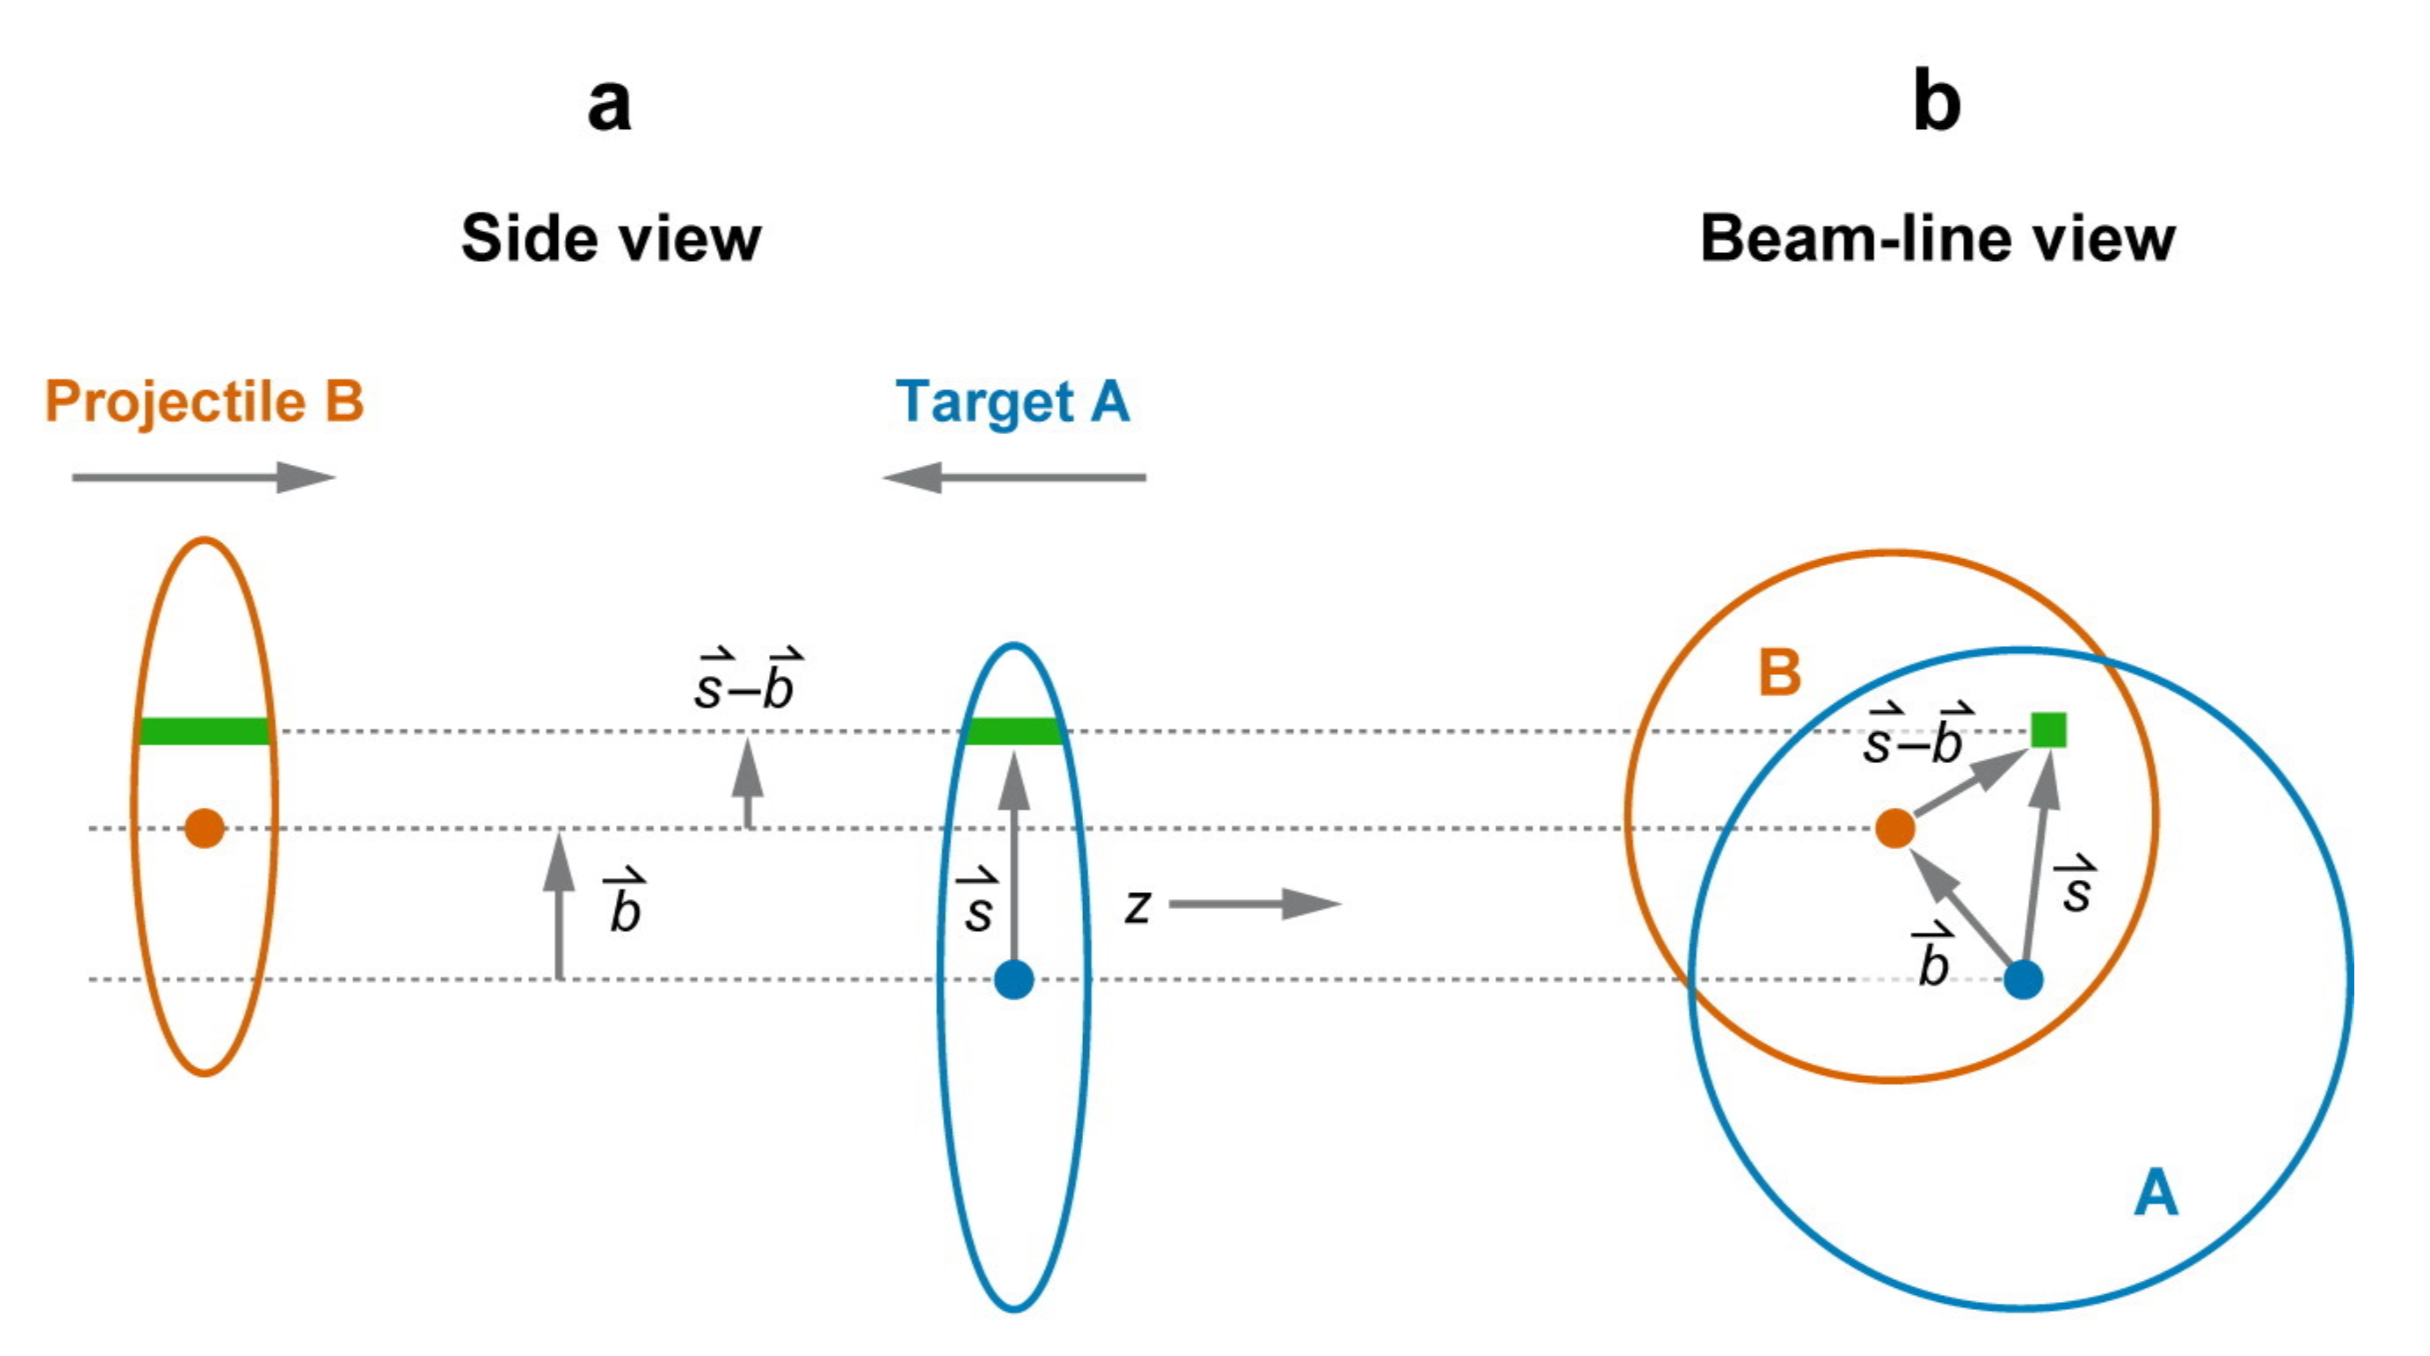
\includegraphics[width=0.8\textwidth]{gfx/glauber}
	\caption{Sketch of the longitudinal and transverse view of an heavy ion collision taken from \cite{glauber}. In the side view, the colliding nuclei are squeezed to represent the Lorentz boost contraction due to their momentum.}
	\label{fig:glauber}
\end{figure}

Following the notation introduced in Figure \ref{fig:glauber} the nuclear overlap function for two colliding
nuclei (A and B) can be written as:
\begin{equation} \label{eq:overlap}
    T_{AB}(\vec{b}) = \int T_{A}(\vec{s})\,T_{B}(\vec{s}-\vec{b}) \mathop{d^{2}s}
\end{equation}
and represents the probability of finding a nucleon in both the colliding nuclei inside the 
overlap region in the transverse plane.
$T_{A}(\vec{s})$ and $T_{B}(\vec{s}-\vec{b})$ are the \textit{thickness functions} the A and B
nuclei.
They represent the probability of finding a nucleon in the unit transverse area located at 
$\vec{s}\xspace$ given the probability per unit volume $\rho(\vec{s},z)$:
\begin{equation} \label{eq:thickfunc}
    T(\vec{s}) = \int \rho(\vec{s},z) \mathop{dz}.
\end{equation}
As assumed, binary only interactions between nucleons are considered and the interaction does not
deflect the trajectory of the interacting nucleons.
Therefore, each nucleons can participate in more than one binary collision. 
The probability of having $n$ binary collisions between the nuclei A and B, having A and B nucleons
respectively, can be computed using the binomial statistics:
\begin{equation} \label{eq:ABprob}
    P(n,\vec{b}) = \frac{AB!}{n! (AB-n)!}[T_{AB}(\vec{b})\sigma_{inel}]^{n} [1-T_{AB}(\vec{b})\sigma_{inel}]^{AB-n}.
\end{equation}
From this expression the total inelastic cross section is obtained as a function of the impact
parameter integrating the double differential cross section for two colliding nuclei:
\begin{equation} \label{eq:doublediff}
    \frac{d^{2} \sigma^{AB}_{inel}(b)}{\mathop{db^{2}}} = \sum_{n=1}^{AB} P(n,b)
    = 1 - [1-T_{AB}(\vec{b})\, \sigma_{inel}]^{AB}
\end{equation}
\begin{equation}
    \sigma^{AB}_{inel}(b) = \int_{0}^{\infty} 2 \pi \, b \mathop{db} \,
    [1 - [1-T_{AB}(\vec{b})\, \sigma_{inel}]^{AB}]
\end{equation}


From eq. \ref{eq:ABprob}, $\mathrm{N}_{coll}$ can be derived as a function of the impact parameter 
summing all the possible numbers of collisions weighted by their own probability and using the
definition of the mean of the binomial distribution:
\begin{equation} \label{eq:ncoll}
    \mathrm{N}_{coll}(b) = \sum_{n=1}^{AB} n\, P(n,b) \ = AB\, T_{AB}\, \sigma_{inel}.
\end{equation}
Similarly $\mathrm{N}_{part}$ can be obtained by integrating over $\vec{s}$ the contribution of the
projectile nucleus and the contribution of the target nucleus as follow:
\begin{equation} \label{eq:npart}
    \mathrm{N}_{part}(b) = \int \mathop{d^{2}s} \, \bigl\{ A\, T_{A}(\vec{s})[1-(1- T_{B}(\vec{b}-\vec{s})\, \sigma_{inel})^{B}
    ] + B\, T_{B}(\vec{b}-\vec{s}) [1-(1-T_{A}(\vec{s})\,\sigma_{inel})^{A}] \bigr\}
\end{equation}
In eq. \ref{eq:ncoll} and \ref{eq:npart}, $\vec{b}$ has been replaced with its norm as the direction 
of the vector is relevant for polarised nuclei only.

In spite of its simplicity, the Glauber Model allows to express $\mathrm{N}_{coll}$ and 
$\mathrm{N}_{part}$ starting from $\rho(\vec{s})$ and $\sigma_{inel}$. The main limitation
is the usage of continuous density functions that implies considering discrete physical quantities 
as continuous.

%
\subsection{Space time evolution of Heavy Ion collisions} \label{sec:1.3.2}

When two ultrarelativistic atomic nuclei collide, high hadron density and high temperatures
are produced in the impact region. 
In these conditions a long lived and strongly interacting system is created.
The evolution of such a system, as well as the characterisation of its properties, is very important
to improve our understanding of the Strong interaction. Hence it is one of the main subject of 
investigation of HI experiments.

\begin{figure}
    \centering
    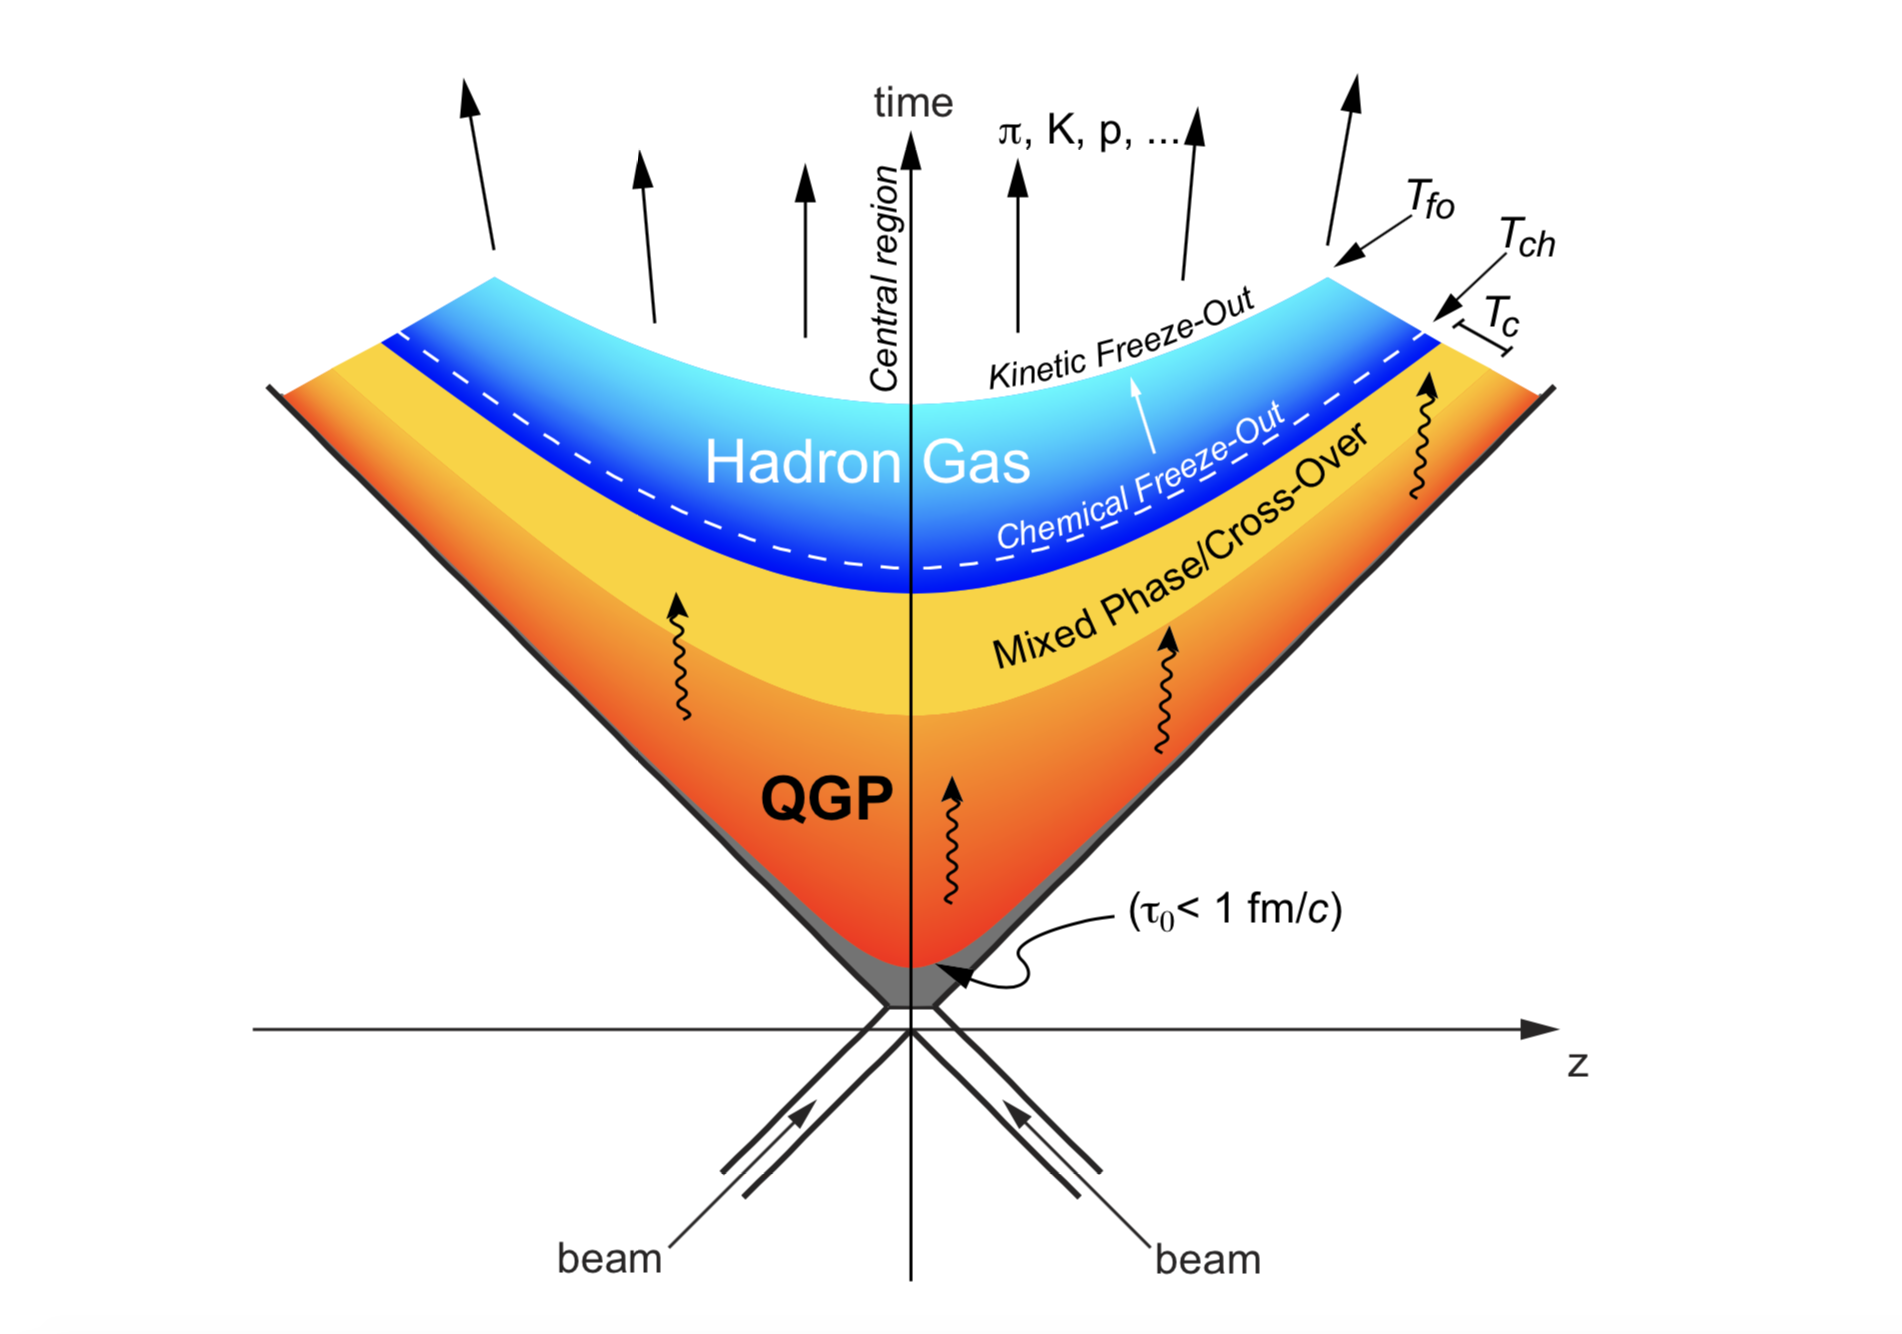
\includegraphics[width=0.9\textwidth]{gfx/evolution}
    \caption{Space-time representation of the evolution of the system created in a central Heavy Ion collision in the mid-rapidity region. The z direction is parallel to the beam line.}
	\label{fig:evolution}
\end{figure}

The space-time evolution of the system (procede) in different phases.
The current view on the evolution is summarized in Figure \ref{fig:evolution}.
\begin{enumerate}
    \item \textbf{\textit{t < 0} fm/\textit{c}:} the two atomic nuclei travel in the beam line. In modern accelerators
        the nuclei are strongly Lorentz contracted in the beam line direction due to their (velocità)
        vicina  aquella della luce (factor of 2700 at the LHC);

    \item \textbf{\textit{t = 0} fm/\textit{c}:} collision time. The geometry of the collision can be described using the Glauber Model described in the previous section;

    \item \textbf{\textit{0 < t}} $\, \pmb{\lesssim \, \text{\Large$ \tau_{0} $} \sim }$ \textbf{\textit{1} fm/\textit{c}:}
            in the early collision stages hard processes (i.e. process with high transferred momentum $Q^{2}$) occur between
            colliding partons. In this phase called \textit{pre–equilibrium}, all the particles with high mass or/and
            high momentum are produced. In high energy collisions, as at the LHC, the nuclei constituent partons 
            lose their energy in the mid-rapidity\footnote{The rapidity is defined, for a particle with four-momentum 
            $p^{\mu} = (E,\vec{p})$, as $y = \frac{1}{2} \log \bigl( \frac{E+p_{z}}{E-p_{z}} \bigr) $, with $z$ parallel
            to the beam direction.} region ($y\approx 0$) and then they escape at forward rapidities ($|y| \gg 0$). 
            The escaping valence quarks bring the baryonic potential carried by the colliding nuclei at forward rapidity,
            vanishing the baryon chemical potential at mid-rapidity.
            The resulting system is an hot and dense medium. If the energy density is high enough, as at the LHC, a 
            transition to the QGP state is expected.
            After a short strong parton rescattering phase, the obtained droplet of QGP matter reaches the equilibrium
            at his proper time $\tau_{0}$;
            
    \item \textbf{\textit{1}} $\, \pmb{\lesssim}$ \textbf{\textit{t}} $\, \pmb{\lesssim}$ \textbf{\textit{10} fm/\textit{c}:}
            the QGP droplet reach the thermal equilibrium and collectively expands under the push of the thermal pressure
            gradients generated at the system boundaries. Relativistic hydrodynamics models \cite{relhydro} are commonly 
            used to describe the rapid expansion of the QGP matter, providing useful insights to interpret the 
            experimental data.
            As a consequence of the expantion, the system cools down and the energy density decreases, transing eventually
            from the Quark Gluon Plasma phase and ordinary hadronic matter;

    \item \textbf{\textit{10}} $\, \pmb{\lesssim}$ \textbf{\textit{t}} $\, \pmb{\lesssim}$ \textbf{\textit{15} fm/\textit{c}:}
            the critical temperature between the two phases is reached. At this temperature the hadronization process
            starts, leading the system into an interacting \textit{hadron resonance gas}. In this stage, the expansion
            and the cooling of the system continue, meanwhile elastic and inelastic interactions among the hadrons
            occour. 
            When the energy density is decreased that much to not allowing inelastic interactions, the relative 
            abundances of different particle species are fixed. The temperature at which the system stops to 
            interact inelastically is called temperature of \textit{chemical freeze-out} T$_{ch}$. After the
            \textit{chemical freeze-out} only elastic processes took place, varying the particles momentum.
            When elestic interactions ends as well, the particles momentum spectra are fixed and this occours
            at the temperature of \textit{kinetic freeze-out} T$_{kin}$;

    \item \textbf{\textit{t}} $\, \pmb{\gtrsim}$ \textbf{\textit{15} fm/\textit{c}:} hadrons created in 
            the collision escape the interaction region with no further interactions. This regime is 
            also known as \textit{free hadron stream}.
\end{enumerate}

The particles produced in the collisions and escaped from the interaction region are detected by 
the experimental apparata carrying informations about the environment in 
which they have been produced and about the medium in which thay have travelled. 
In the following it will be shown how properties of the systems and characteristics of its 
evolution can be inferred by the measurement of particle production spectra and particle correlations.

%
%
\section{Nuclei production in Heavy Ion collisions} \label{sec:1.4}

The main subject of this thesis is the study of the \dst dibaryon production at the LHC energies.
Except for the deuteron, dibaryons are little known objects. In the next chapter, more details
on what dibaryons are and what our understanding is about dibaryons, will be provided. 

The (anti-)nuclei are loosely bound objects and it is not trivial how they can emerge from Heavy 
Ion collisions. 
The following sections are dedicated to a brief description of the major two classes of models
that try to explain the nuclei and anti–nuclei production in HI collisions: the Statistical 
Hadronisation Models (SHMs) and the Coalescence model \cite{deuprod}.
Dibaryons and in particular \dst \ \ -- which can be considered as an excited deuteron -- \ should 
be subject of same production mechanisms as for (anti-)nuclei.

%
\subsection{Statistical Hadronisation Models} \label{sec:1.4.1}

The Statistical Hadronisation Models (also known as Thermal Models) was successfully developed
in order to describe the abundances of different particle species produced in the collision 
between particles.

The general idea behind these models is that the final state of the interaction is composed by
all the particle states compatible with the conservation laws imposed by the underlying theory 
of interaction (in our case the Standard Model of particle physics). 
The relative abundance of different particle states is set by the maximisation of the total phase
space filled by the system, to which each particle species contributes according to its partition 
function. These models are of particular interest in HI collisions as the presence of an expanding 
medium that eventually reaches the thermal equilibrium seems appropriate for the statistical
hadronisation approach. 

The system created in a relativistic HIC is large enough to be modelled using the Grand Canonical
ensemble. 
This formalism can be used as the central rapidity region is in equilibrium with a thermal reservoir 
(the rest of the medium created in a HI collision) and quantities like energy, baryon number, 
charge and isospin are conserved on average. Most of the barrel experiments (as for ALICE central
detectors) measure only this part of the phase space, hence the use of the Grand Canonical formalism 
is allowed.
Within this formalism the parameters describing the equilibrium condition of a HIC
include the temperature T and the baryon chemical potential $\mu_{B}$. On this basis 
the partition function of the system can be written as:
\begin{equation} \label{eq:partfunction}
    Z(T,V,\mu) = \Tr \Big[ e^{-\beta(H-\Sigma_{i}Q_{i}\mu_{i})} \Big]
\end{equation}
with
\begin{equation}
    \mu = \sum_{i} Q_{i} \mu_{Q_{i}} \ \ \ \mathrm{and} \ \ \ \beta = \frac{1}{T}
\end{equation}
where $V$ is the volume of the system at equilibrium, $H$ is the
Hamiltonian and $\mu_{Q_{i}}$ is the chemical potential associated to the conserved quantum number
$Q_{i}$.
For a strongly interacting medium, the main conserved quantum numbers are the electric charge $Q$,
the strangeness content of the system $S$ and the baryon number $B$.
The Hamiltonian $H$ in the partition function is that one of a Hadron Resonance Gas since it is able 
to describe the behaviour of a strongly interacting medium reproducing over a wide temperature range
the equation of state obtained with lQCD calculations before the transition to a deconfined state.
The choice of the mesonic, baryonic and resonance states included in the Hamiltonian depends on the
implementation of the model and it determines the maximum temperature that can be described accurately.

The partition function of the system is the product of the contribution of all the particle states
in the Hadron Resonance Gas:
\begin{equation} \label{eq:partfuncprod}
    Z(T,V,\mu) = \prod_{i} Z_{i}(T,V,\mu_{i}) \ \ \ \rightarrow \ \ \ 
    \log Z(T,V,\mu) = \sum_{i} \log Z_{i}(T,V,\mu_{i}).
\end{equation}
The partition functions are defined by the spin–statistics theorem:
\begin{equation} \label{eq:partfuncspin}
    \log Z_{i}(T,V,\mu_{i}) = \frac{V g_{i}}{2 \pi^{2}} \int_{0}^{\infty}\
     \pm p^{2} \mathop{dp} \, \log \Big[1\pm \lambda_{i}(T,\mu_{i})e^{- \beta \epsilon_{i}} \Big]
\end{equation}
Bose-Einstein distribution for bosons ($+$) and Fermi-Dirac distribution for fermions ($-$).
The $g_{i}$ constant is the degeneracy state $i$ and $\epsilon_{i}$ is the energy of one 
particle of the species $i$ with momentum $p (\epsilon_{i} = \sqrt{p^{2} + m_{i}^{2}})$.
The dependence on the chemical potentials is encoded within the \textit{fugacity}
$\lambda_{i}$:
\begin{equation} \label{eq:fugacity}
    \lambda_{i}(T,\mu_{i}) = e^{\beta(B_{i}\mu_{B} + S_{i}\mu_{S} + Q_{i}\mu_{Q})}
    = e^{\beta \mu_{i}}
\end{equation}
where $B_{i}$, $S_{i}$ and $Q_{i}$ are the baryon number,strangeness content and electric
charge associated with the particle species and $\mu_{B}$ , $\mu_{S}$ and $\mu_{Q}$ are the 
respective chemical potentials. As described in \cite{pbmstat}, expanding the logarithm and
integrating over the momentum, the partition function for the species $i$ becomes:
\begin{equation}
    \log Z_{i}(T,V,\mu_{i}) = \frac{V T g_{i}}{2 \pi^{2}}
    \sum_{k=1}^{\infty} \frac{(\pm 1)^{k+1}}{k^{2}} \lambda^{k}_{i} m_{i}^{2} K_{2}(\beta k m_{i})
\end{equation}
where the ($+$) is for bosons, the ($-$) for fermions and the $K_{2}$ is the second 
kind modified Bessel function of second order.

The average number of particle for the species $i$ for a system described by the Gran
Canonical ensemble, is defined as:
\begin{equation} \label{eq:particleyields1}
    \langle N_{i} \rangle ^{th} (T,V,\mu_{i}) = \frac{1}{\beta} \frac{\partial}{\partial \mu_{i}}
    \log Z_{i}(T,V,\mu_{i})
    \frac{V T g_{i}}{2 \pi^{2}}
    \sum_{k=1}^{\infty} \frac{(\pm 1)^{k+1}}{k} \lambda^{k}_{i} m_{i}^{2} K_{2}(\beta k m_{i}).
\end{equation}
This equation does not fully describe the particle abundances measured in HI callisions.
For the measured yields one should consider the feed–down contributions from all the other
particle species (resonances) $j$ in the thermal system that can decay strongly in a final
state containing particles of the species $i$:
\begin{equation} \label{eq:particleyields2}
    \langle N_{i} \rangle ^{th} (T,V,\mu) = \langle N_{i} \rangle ^{th} (T,V,\mu_{i})
    + \sum_{j} \Gamma_{j \to i} \langle N_{j} \rangle ^{th} (T,V,\mu_{j})
\end{equation}
where $\Gamma_{j \to i}$ is the decay rate of the state $j$ into the final state $i$.

The definition of particle yields is valid in the limit of a low density system, 
where the repulsion interaction between the hadrons constituting the systems is negligible.
The treatment of these interactions is still matter of active theoretical research. Nevertheless 
Eq \ref{eq:particleyields2} and \ref{eq:particleyields1} already indicate the crucial 
dependencies of the observed particle yields on the
temperature $T$, volume $V$ and the chemical potentials $\mu_B$, $\mu_Q$ and $\mu_S$.

Heavy Ions collisions no net strangeness is present in the colliding nuclei, thus 
$\mu_S = 0$, and $\mu_Q$ is fixed by the isospin asymmetry in the collision.
Therefore two of the five parameters of the model are constrained by the collisions
conditions.
The baryon chemical potential $\mu_B$ is not constrained as the "amount of baryonic number"
transported in the equilibrium region depends on the energy of the collision.
The dependence on the volume $V$ of the system can be removed looking at ratio between 
the yields of different particle species, which therefore depends only on the temperature 
of the system and on the baryon chemical potential.
\begin{figure} 
    \centering
    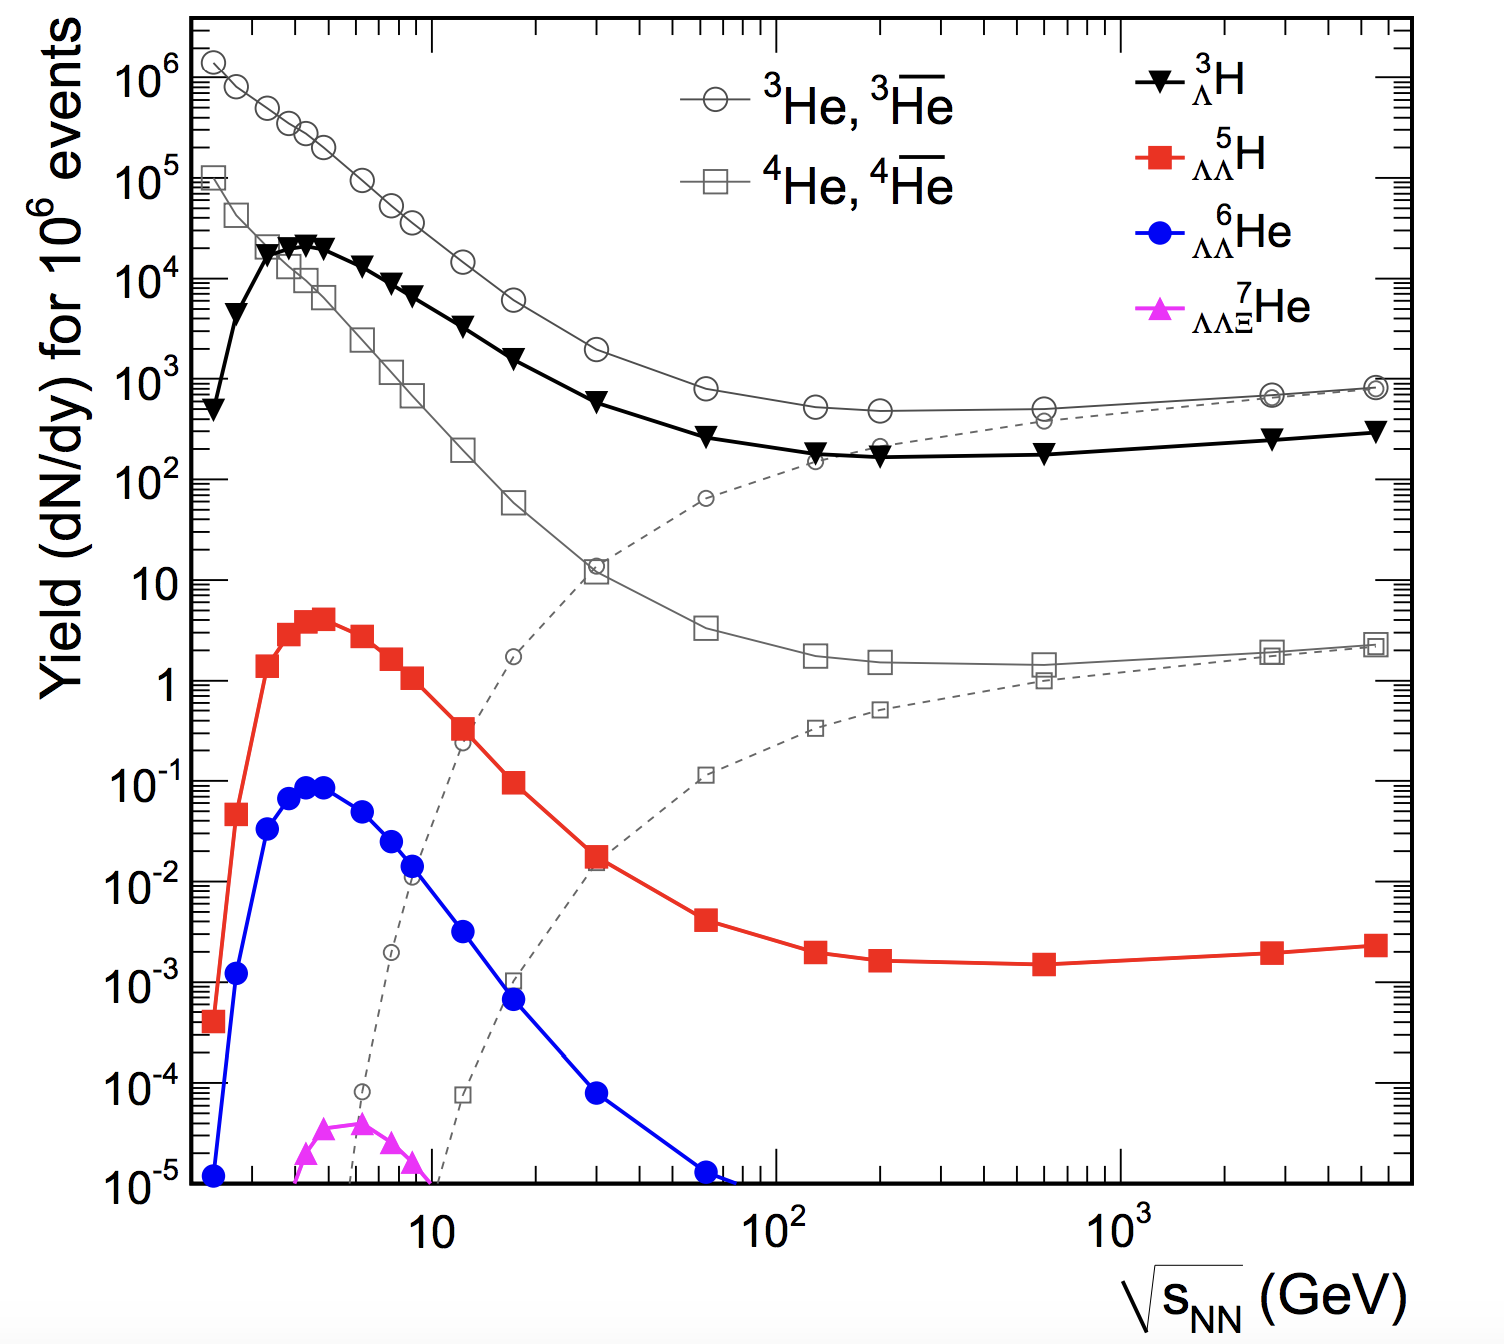
\includegraphics[width=0.7\textwidth]{gfx/yields}
    \caption{Thermal model predictions for the production of various nuclei, anti-nuclei and hyper–nuclei as a function of the ion collision energy taken from \cite{yields}. At low collision energy the baryon chemical potential differs significantly from zero and the particle yield favours matter over anti–matter. As the energy increases, $\mu_{B}$ decreases and this difference vanishes.
}
\label{fig:aliceyields}
\end{figure}
In the framework of the thermal models, light nuclei yields arise naturally when the chemical 
freeze–out temperature and the baryon chemical potential are set.
A possible explanation on how the light nuclei can survive to the high temperature of the chemical 
freeze–out was pointed out in \cite{yields}: as the system expansion after the chemical freeze–out
is supposed to conserve the entropy density, such conservation could be the steering mechanism for 
the nuclei production. From the fit of the particle abundances at lower energies, the 
authors of \cite{yields} predicted, using the thermal model, the yields of (anti-)nuclei 
at the LHC energy \ref{fig:aliceyields}.

%
\subsection{Coalescence Models} \label{sec:1.4.2}

Coalescence models \cite{deuprod} represent a different theoretical approach developed to explain 
the measured light nuclei production in Heavy Ions collisions. 
These models address the problem guessing that light nuclei are created at the kinetic freeze-out. 
They are static models and there is no attempt to give a detailed description of the 
interactions that lead to their formation.
The fundamental idea behind these predictions is that if nuclei constituents are close enough in 
phase space at the kinematic freeze-out they can bind to form a nucleus. 
The coalescence models make a prediction about the momentum distribution of the produced light 
nuclei as a function of the production spectra of the constituents.

The first coalescence model was developed to describe the deuteron formation in
proton-nucleus collisions in 1961, in the following years has been extended to 
the production of various light nuclei in nucleus-nucleus collisions.
The momentum spectrum for the $i$ species related is linked to the proton momentum spectrum,
which is used as a proxy of the constituent spectrum, by the following equation:
\begin{equation}
    E_{i} \frac{d^{3}N_{i}}{\mathop{dp_{i}^{3}}} = B_{A} \Big( E_{p} \frac{d^{3}N_{p}}{\mathop{dp_{p}^{3}}} \Big)^{A}.
\end{equation}
The proton spectrum is assumed to be identical to that one of the constituent neutron.
One of the main reasons behind this generalization is that proton spectra are easier to measure
in an experiment.
These nucleon spectra are not those measured in the experiments, but the ones produced in the 
collision and not yet modified by the coalescence mechanism.
The coalescence parameter $B_{A}$ is interpreted as a function of the radius $p_{0}$, that 
is the maximum distance at which coalescence can happen.
In the simplest formulation of the coalescence models only the momentum space is considered
(not the space-time), thus the coalescence parameter can be expressed neglecting the spin:
\begin{equation} 
    B_{A} = \Big( \frac{4}{3}\, \pi \,p_{0}^3 \Big)^{A-1} \frac{m_{i}}{m_{p}^{A}}.
\end{equation}
where $p_{0}$ is the aforementioned radius and $m_{i}$ and $m_{p}$ are the nucleus and proton
mass, respectively.

More sophisticated versions of this model predict a dependence on the geometry of the system
and rely on different constituents momentum spectra and different formulation of 
the coalescence parameter $B_{A}$. Nevertheless, thanks to its simplicity and the presence
of just one parameter $p_{0}$, the most commonly used for the comparison with the data is
the simple model briefly shown above.
		% INCLUDE: introduction on HENP
% !TEX root = ../main.tex
%
\chapter{The ALICE experiment}
\label{sec:3}

\cleanchapterquote{Alice had begun to think that very few things indeed were really impossible.}{Lewis Carrol}{(Alice's Adventures in Wonderland)}

The Large Hadron Collider (LHC) is the biggest and most powerful particle collider in the world.
It consists of a 27 km ring of superconducting magnets and accelerating structures able to
provide proton-proton and Lead-Lead collisions at the highest energies ever reached in laboratory. At those energies the formation of the Quark Gluon Plasma is expected to happen.
While most of the LHC uptime is dedicated to the proton–proton physics that led to the discovery of 
the Higgs Boson \cite{atlashiggs,cmshiggs} and of two charmed pentaquark states \cite{lhcbpenta}, 
a significant part of the physics programme at the LHC is dedicated to heavy-ion physics and the 
characterization of the Quark Gluon Plasma.

\section{The Large Hadron Collider} \label{sec:3.1}

The Large Hadron Collider is the last element of the accelerator complex at CERN (Figure \ref{fig:lhc})
, a sequence of machines that accelerate particles to increasingly higher energies. Each element in
this chain boosts the energy of a particles beam, before injecting it into the next machine. 
Protons and heavy ions are brought to their collision energies through different acceleration chains.

\begin{figure}
    \centering
    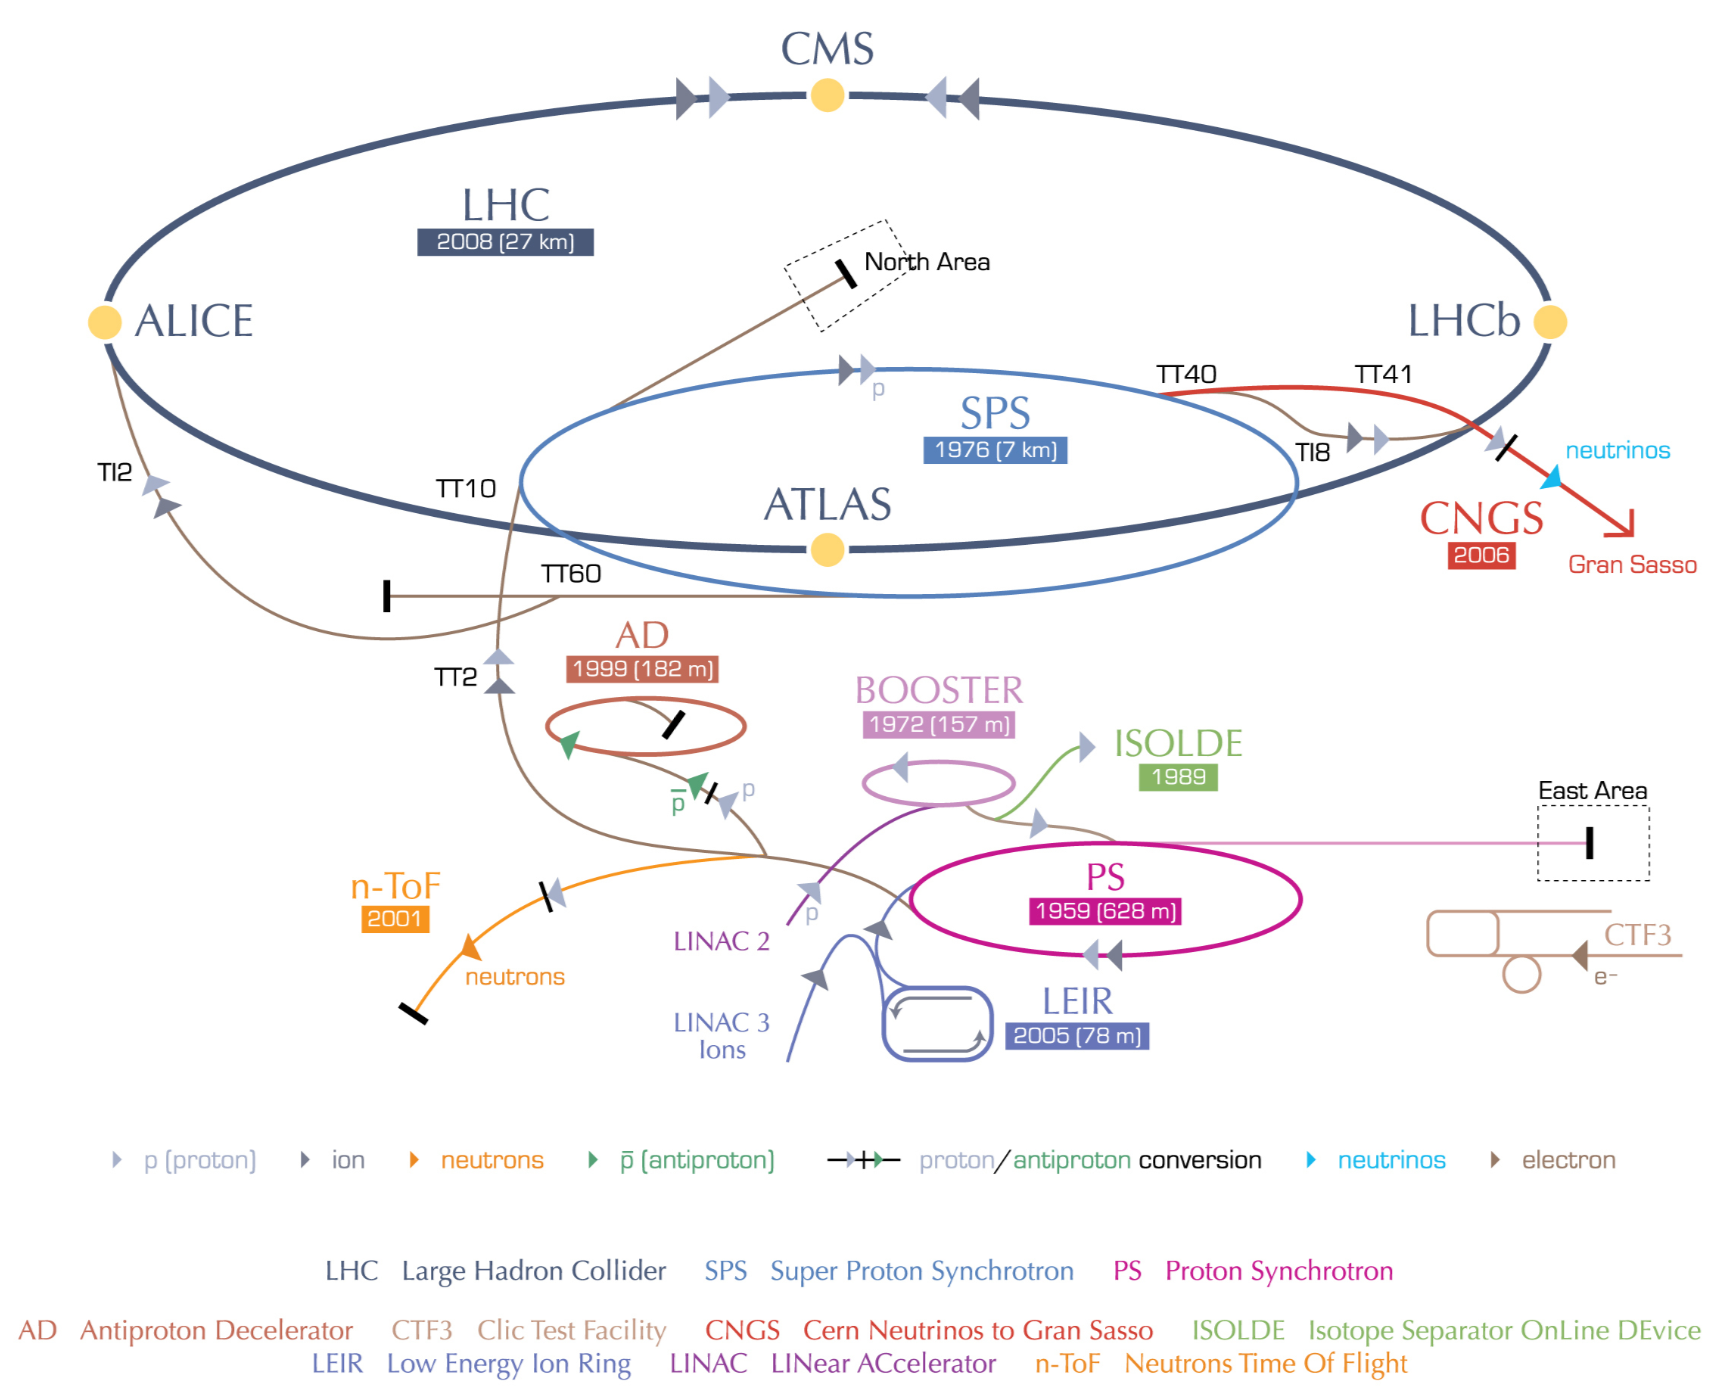
\includegraphics[width=0.8\textwidth]{gfx/lhc}
	\caption{Schematic view of the CERN accelerator complex and the LHC experiments \cite{lhc}.}
	\label{fig:lhc}
\end{figure}

The protons injected in the LHC ring starts their path in the LINAC2, where ionized hydrogen
atoms are accelerated up to 50 MeV. Then the beam is injected in the Proton Synchrotron Booster 
(PSB), which accelerates protons up to 1.4 GeV and provides the beam bunches to the Proton 
Synchrotron (PS). The Proton Synchrotron provides 25 GeV protons to the Super Proton Synchrotron
(SPS), where they are accelerated up to 450 GeV before the injection in the LHC.

Lead ions are produced from a highly isotopically pure $^{208}$Pb sample heated to a temperature
of about $800\,^{\circ}\mathrm{C}$.
The lead vapour is ionized by an electron current. Many different charge states are produced
with a maximum around Pb$^{29+}$.
These ions are selected and accelerated up to 4.2 MeV/u (energy per nucleon) before passing through
a carbon foil, which strips most of them to Pb$^{54+}$. The Pb$^{54+}$ beam is accumulated, then
accelerated to 72 MeV/u in the Low Energy Ion Ring (LEIR), which transfers them to the PS.
The PS accelerates the beam to 5.9 GeV/u and sends it to the SPS after the beam has passed through a second foil where it is fully stripped to Pb$^{82+}$. 
The SPS accelerates the beam to 177 GeV/u and then the beam is sent to the LHC, which accelerates it to 2.56 TeV/u.

The LHC ring is composed by 1232 dipole magnets and 392 quadrupole magnets, which respectively 
guide and focus the counter–rotating beams in separate vacuum–filled pipes.
When the beams are stable they are brought into collision in four interaction points corresponding
to the experimental areas where the major LHC experiments are installed.
The top centre–of–mass energy reached at the LHC in the collisions are 13 TeV and 5.02 TeV per 
nucleon pair for pp and Pb--Pb collisions, respectively.

Besides the centre–of–mass energy another crucial parameter for a collider is the luminosity delivered 
to the experiments.
Indeed the number of events per second generated in the LHC collisions can be evaluated with the
following formula:
\begin{equation}
    R_{event} = L\;\sigma_{event}
\end{equation}
where $L$ is the machine instantaneous luminosity and $\sigma_{event}$ is the cross section for
the event under study. The instantaneous luminosity depends only on the beam parameters and can be 
written as:
\begin{equation}
    L = \frac{N_{b}N^{2} f_{rev} \gamma}{4\,\pi \epsilon_{n} \beta^{*}} F,
\end{equation}
where $N_{b}$ is the number of bunches in the collider ring, $N$ is the number of charges in each
bunch, $f_{rev}$ is the revolution frequency of the beam, $\gamma$ is the relativistic factor,
$\epsilon_{n}$ is the normalized emittance\footnote{$\epsilon_{n} = \beta \gamma \epsilon$ 
where $\beta$ and $\gamma$ are the usual relativistic factors and the emittance $\epsilon$ is the
spread of beam particles in the position-momentum phase space.} and $\beta^{*}$ is the value 
of the amplitude function\footnote{The amplitude function $\beta(s)$ describes the beam 
amplitude modulation due to the changing focusing strength.} at the interaction point (IP)
where the luminosity is estimated.

\begin{figure}
    \centering
    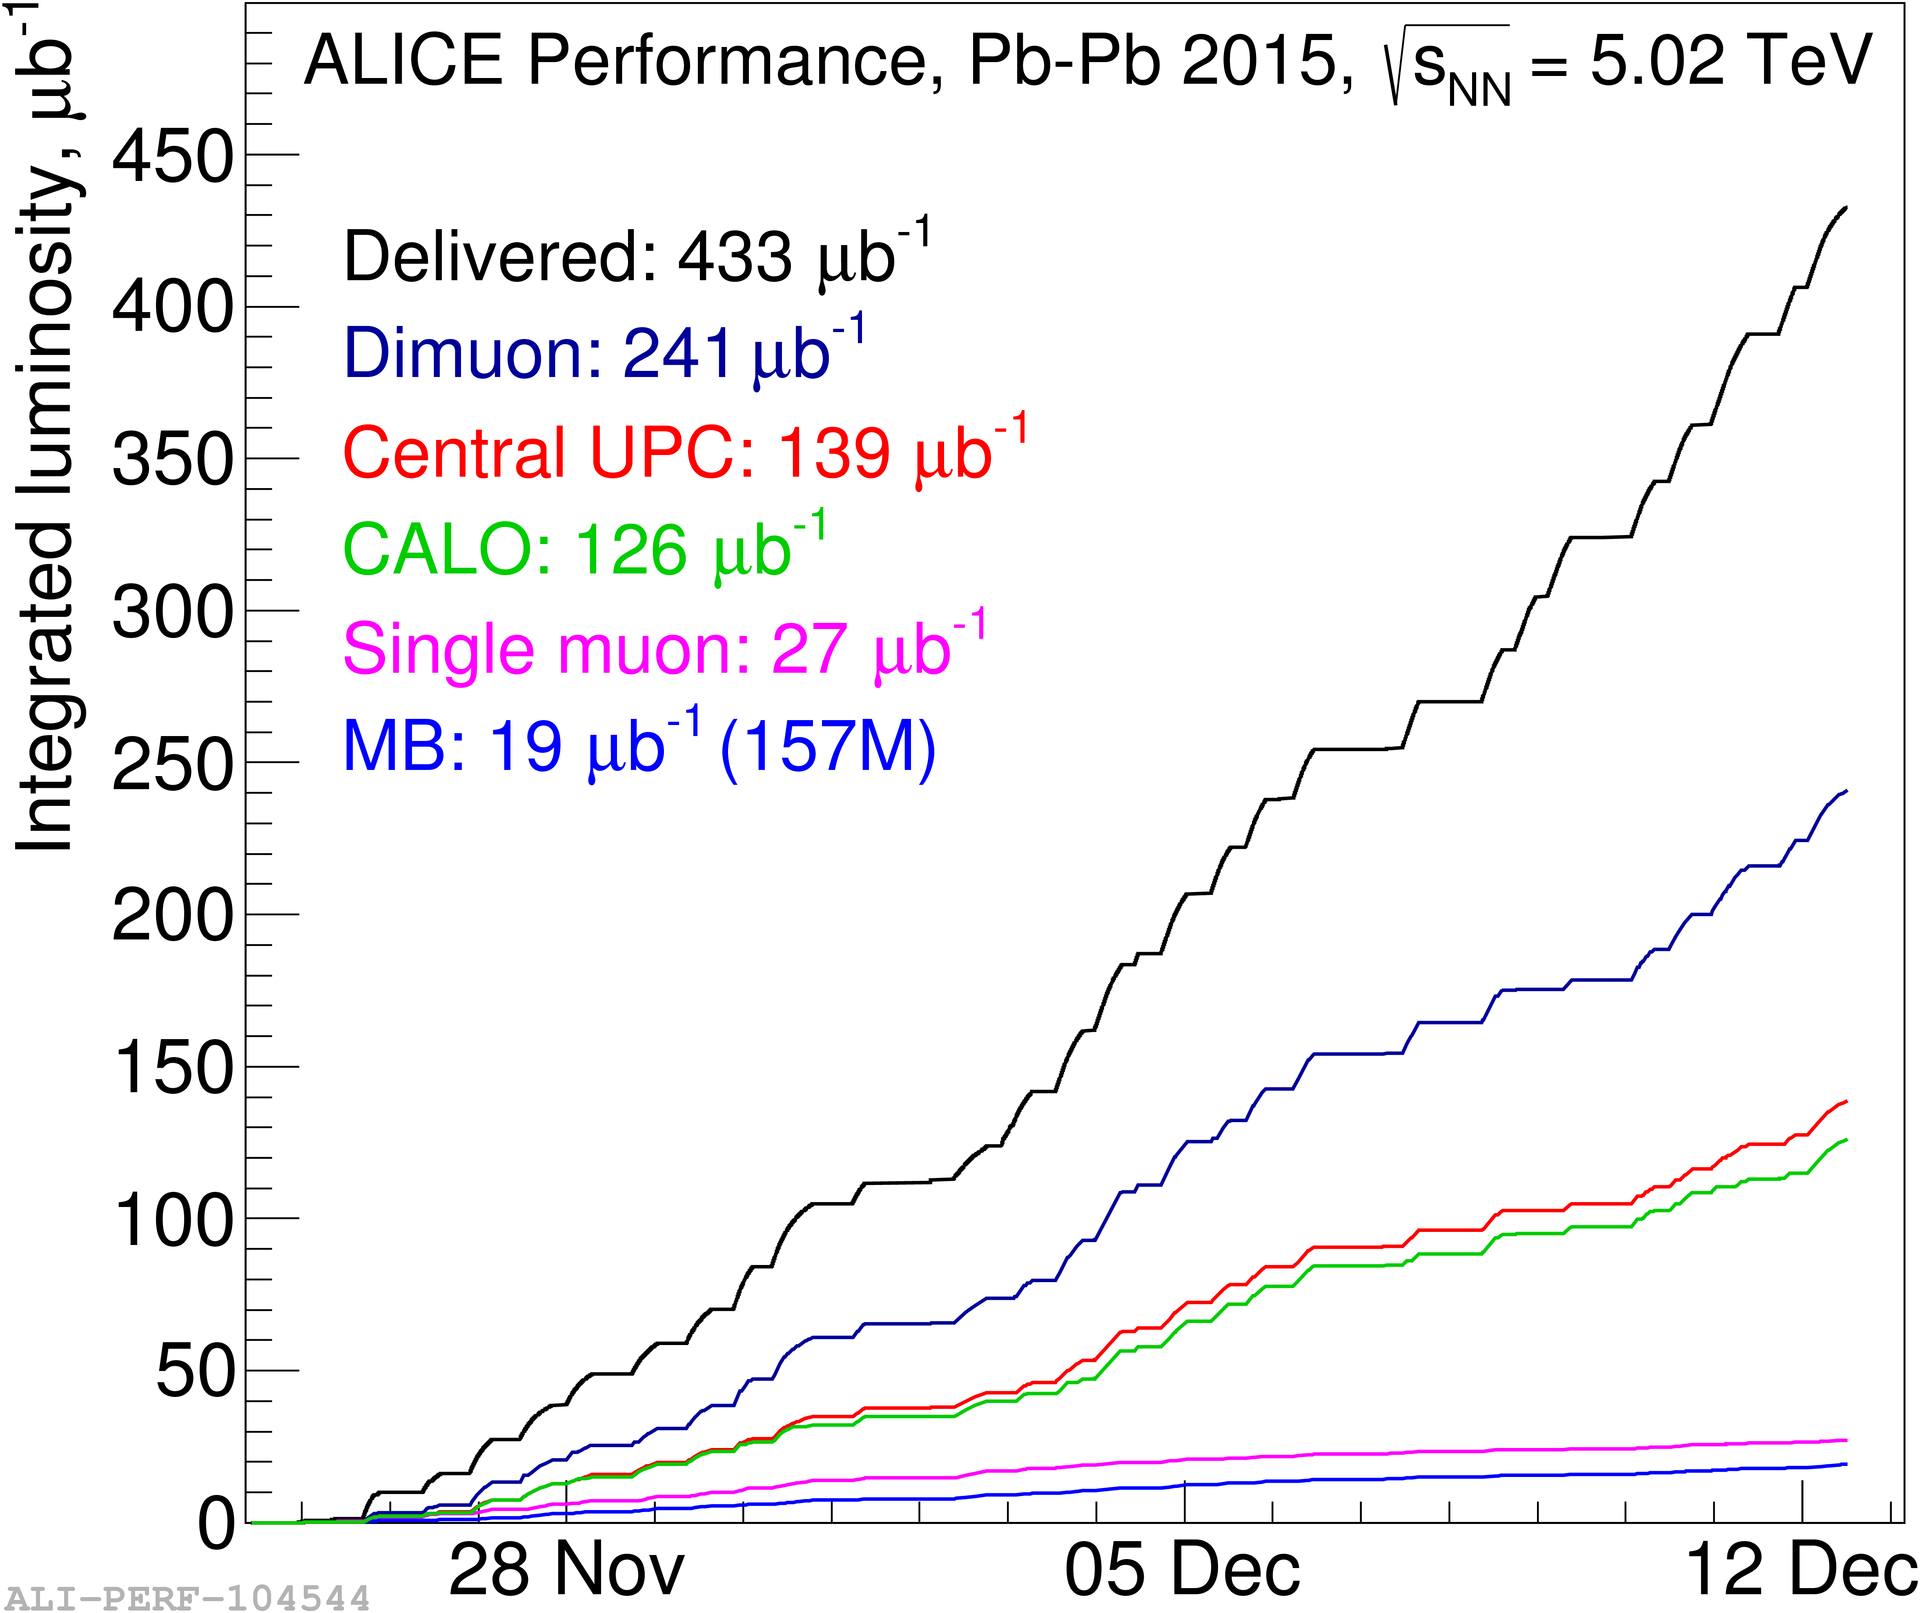
\includegraphics[width=0.6\textwidth]{gfx/alicelumi}
	\caption{ALICE delivered and integrated luminosity during the first Pb–Pb period in Run 2.}
	\label{fig:alicelumi}
\end{figure}

In order to maximise the luminosity of the LHC, the option of a p$\bar{\mathrm{p}}$ collider
was excluded due to the problem of the anti–protons production that is very complicated.
The LHC can store up to 2808 bunches, with $\sim 10^{11}$ protons per bunch, with 25 ns spacing
\cite{lhcperf}.
The ALICE apparatus requires a peak luminosity of $L = 10^{27}$ cm$^{-2}$s$^{-1}$ in Pb--Pb collisions.
Figure \ref{fig:alicelumi} shows the delivered luminosity by the LHC (black line) and the integrated
luminosities collected by ALICE, for different trigger configurations (coloured lines), during the
first Pb–Pb period in Run 2 at the end of 2015.

A crucial information for the collider experiments is the position where the collision
between the two beams takes place: the \textit{primary vertex}. 
The nominal position of the primary vertex is the origin of the coordinate reference frame of the 
experiment. Nevertheless, due to the finite size of the bunches the position of the primary
vertex fluctuates around the nominal position.
Being $\sigma^{bunch}_{x,y,z}$ the \textit{rms} of the bunch in the transverse and longitudinal
direction, it can be shown that, assuming a gaussian profile of the bunches in the three directions,
the \textit{rms} of the vertex variation is:
\begin{equation}
    \sigma^{vertex}_{x,y,z} = \frac{\sigma^{bunch}_{x,y,z}}{\sqrt{2}},
\end{equation}
where the \textit{rms} size depends on the beam emittance and the amplitude function $\beta^{*}$:
\begin{equation}
    \sigma^{bunch}_{x,y,z} = \sqrt{\frac{\epsilon_{x,y,z}\,\beta^{*}}{\sqrt{\pi}}}.
\end{equation}
At the Interaction Point 2 (IP2), where the ALICE experiment is located, typical values for the vertex dispersion are 
$\sigma^{vertex}_{x,y}\,\sim 50\;\mu\mathrm{m}$ and $\sigma^{vertex}_{z}\,\sim 5\;\mathrm{cm}$.

%
%
\section{ALICE design} \label{sec:3.2}

The main goal of the ALICE experiment is the study of the QCD matter created in high energy heavy
ion collisions, hence the detector has been designed and optimised \cite{alicedesign1,alicedesign2}
for this purpose.
A heavy ion experiment must have an efficient tracking system with a large acceptance and a good
particle identification (PID) capabilities in a wide momentum range, especially at low momentum.
Furthermore, it has to work in an environment characterized by a large charged particle multiplicity.
At the time of ALICE design, the charged particles multiplicity per rapidity unit in central Pb–Pb 
collisions was predicted to range between 2000 and 8000 \cite{alicemulti}, and for this reason
detectors with high granularity and low material budget have been developed 
\cite{alicedesign1,alicedesign2}.

The current layout of the ALICE experiment is shown in Figure \ref{fig:alice3D} while Table 
\ref{tab:alice} lists the position and the purpose of the ALICE sub-detectors.
\begin{figure}
    \centering
    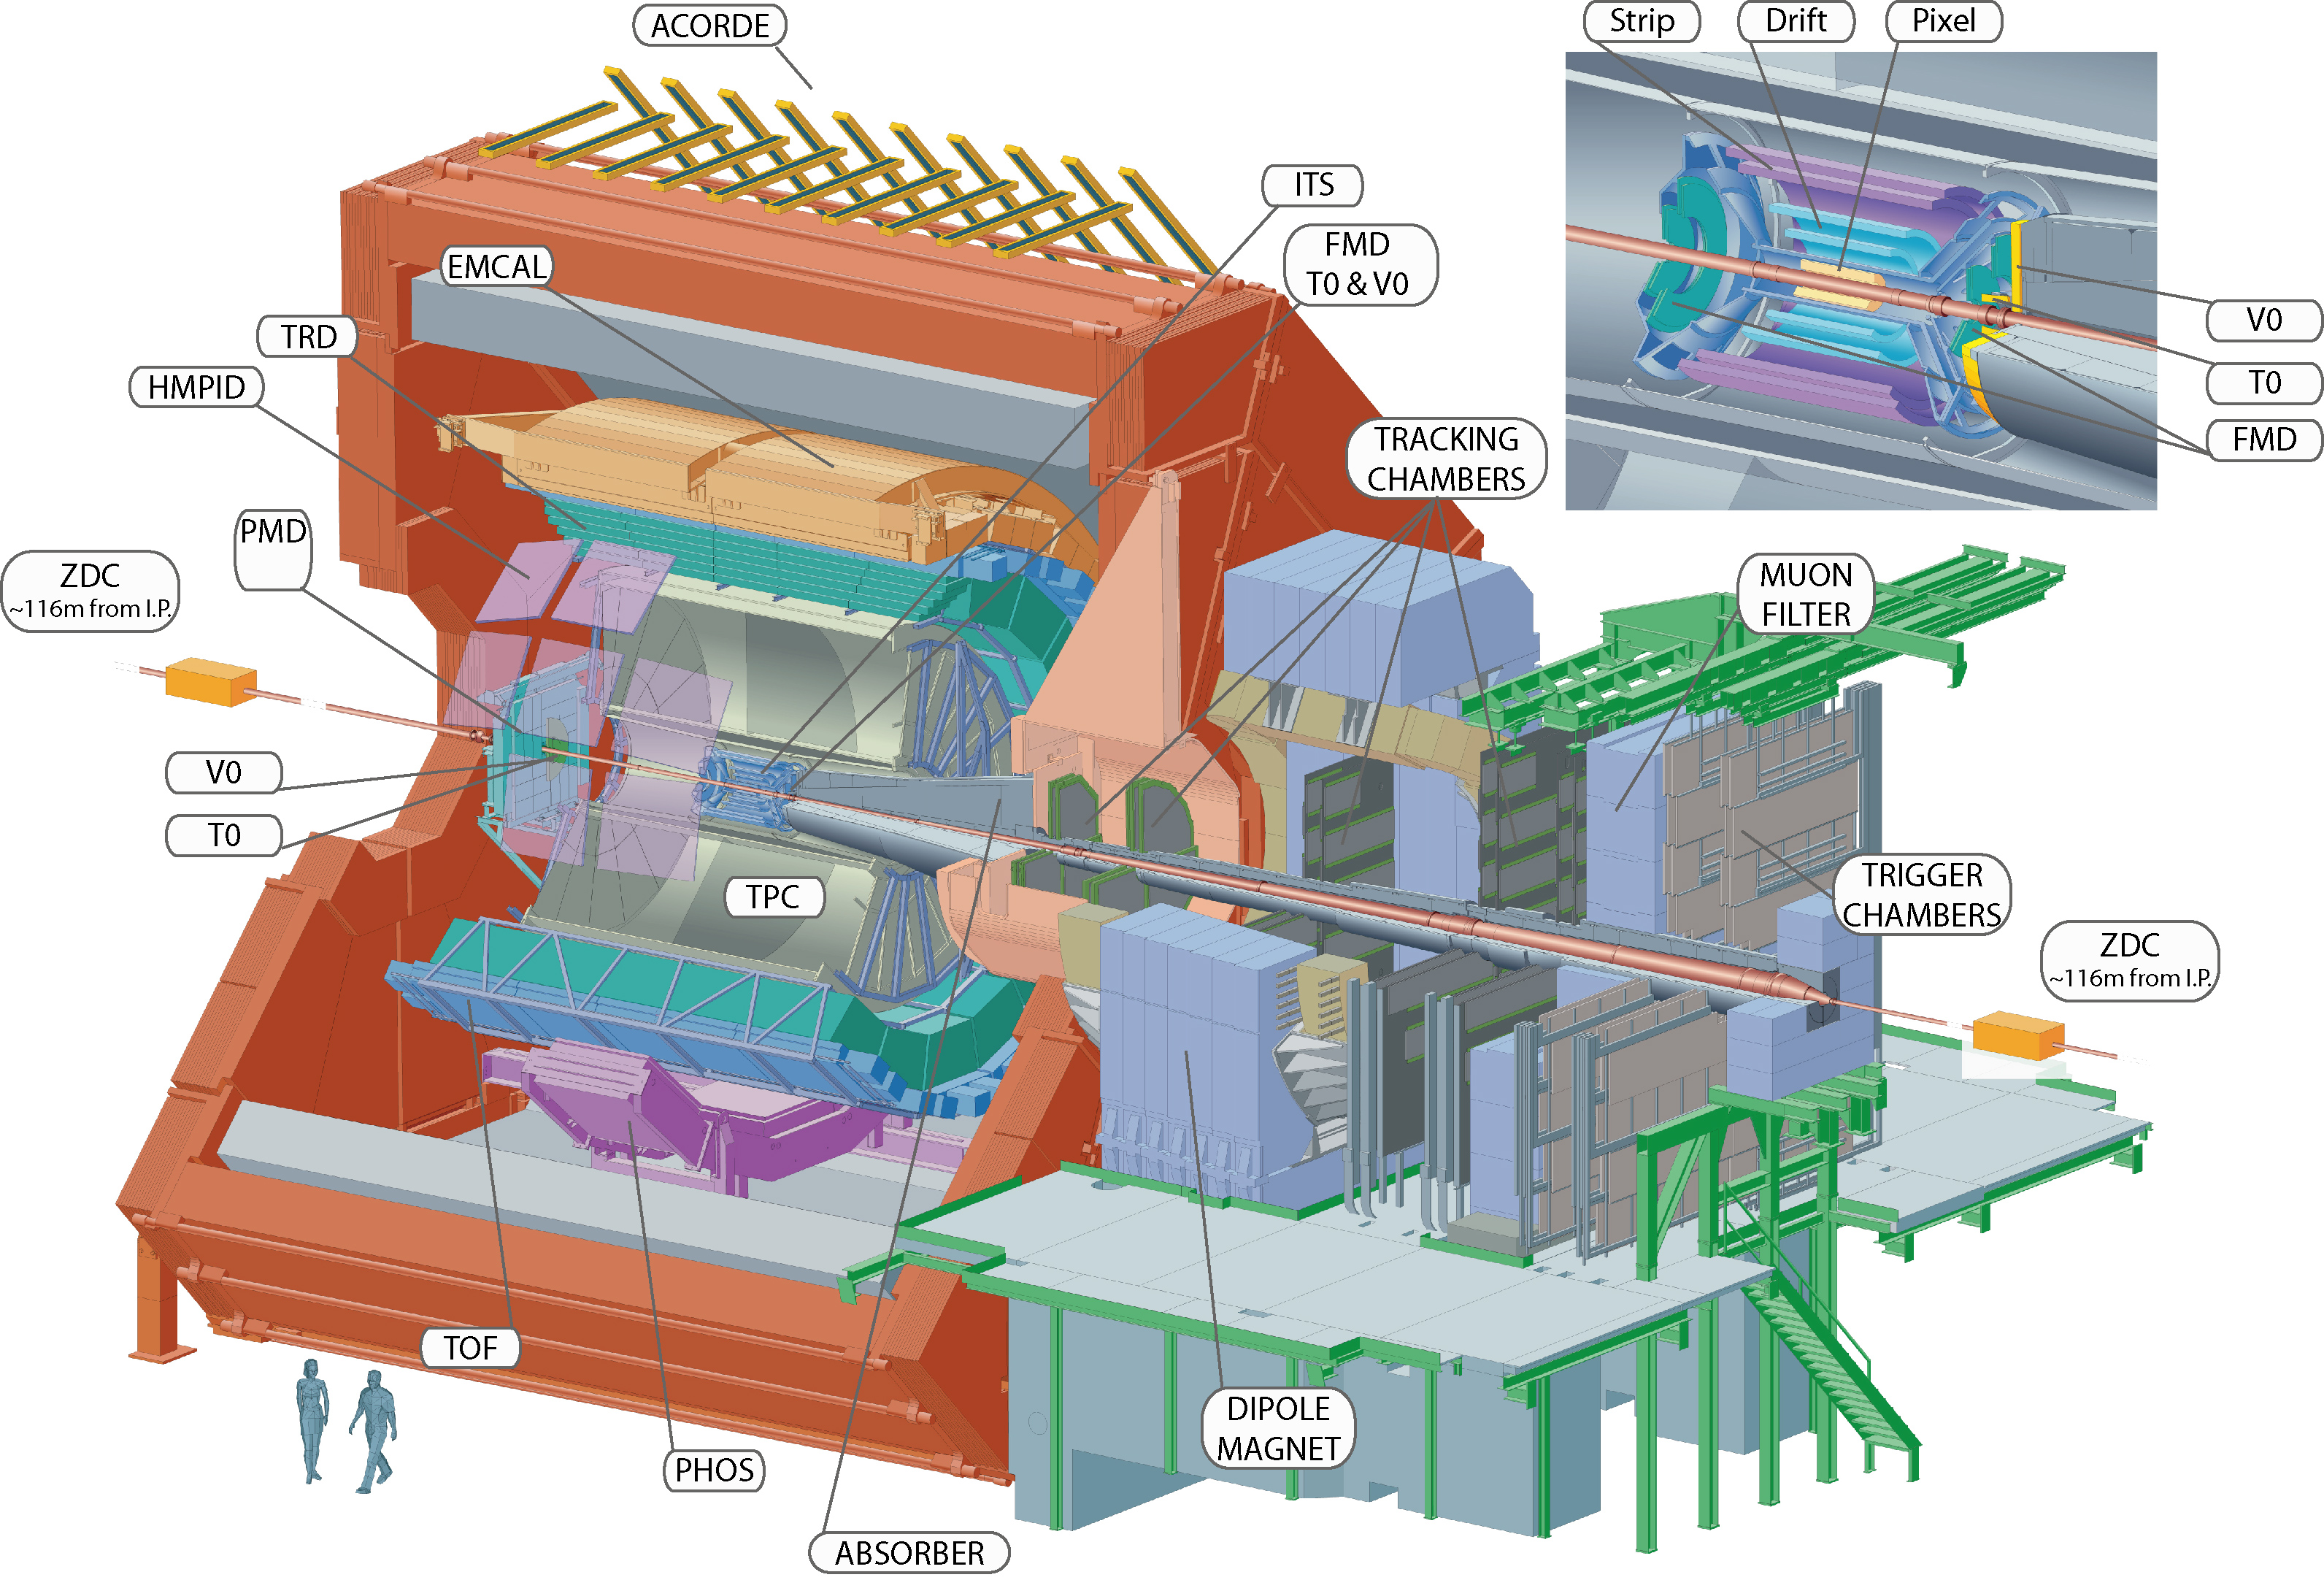
\includegraphics[width=0.9\textwidth]{gfx/alice3D}
	\caption{The ALICE experimental setup and the red L3 solenoid magnet. The top right inset shows a zoom on the V0, T0, FMD and the ITS detectors.}
	\label{fig:alice3D}
\end{figure}
The ALICE coordinate system is a right-handed orthogonal Cartesian system with the origin settled at
the nominal beams interaction point.
The $x$ axis is aligned with the horizontal accelerator plane and points to the centre of the LHC,
the $y$ axis is perpendicular to the accelerator plane and points upward.
As a consequence the $z$ axis is parallel to the beam direction and its positive direction is 
defined by the chirality of the coordinate system. 
For a more useful description of the apparatus and the physical quantities, two other coordinates
are defined, which together with the $z$ axis described above, form a cylindrical coordinate system:
the azimuthal angle $\phi$ increases counter-clockwise starting from $\phi = 0$ for $x$ axis looking
towards the CMS side, and the polar angle $\theta$ increases from $z$ ($\theta=0$) to $-z$ 
($\theta=\pi$).
Other two useful variables, widely used in this thesis, are the \textit{pseudo-rapidity} $\eta$:
\begin{equation}
    \eta = \frac{1}{2} \ln \frac{|p| + p_{z}}{|p| - p_{z}} =
     - \ln \left[ \tan \left(\frac{\theta}{2} \right) \right],
\end{equation}
and the \textit{rapidity}:
\begin{equation} \label{eq:rapidity}
    y = \frac{1}{2} \log \bigl( \frac{E+p_{z}}{E-p_{z}} \bigr) 
\end{equation}
for a particle with four-momentum $p^{\mu} = (E,\vec{p})$, and the $z$ axis parallel to the beam 
direction.
For ultra-relativistic objects, the \textit{pseudo-rapidity} numerically converges to the 
\textit{rapidity}.

\begingroup
\setlength{\tabcolsep}{6pt} % Default value: 6pt
\renewcommand{\arraystretch}{1.5} % Default value: 1
\begin{table}[!tp]\small
\centering
	\begin{tabular*}{\textwidth}{@{\extracolsep{\fill}}lcccc}
	\toprule
		     & \multicolumn{2}{c}{\normalsize{\textbf{Acceptance}}} \\
	\textbf{\normalsize{Detector}} & \textit{\textbf{Polar}} & \textit{\textbf{Azimuthal}} & \textbf{\normalsize{Position}} & \textbf{\normalsize{Main purpose}}	 \\
    \midrule
	SPD$^{\dagger}$	\textit{layer 1}     & $|\eta|$ < 2.0	  & full			& r = 3.9 cm		& tracking, vertex\\
	SPD$^{\dagger}$	\textit{layer 2}     & $|\eta|$ < 1.4	  & full			& r = 7.6 cm		& tracking, vertex\\
	SDD	\textit{ layer 3}		         & $|\eta|$ < 0.9	  & full			& r = 15 cm		    & tracking, PID\\
	SDD	\textit{ layer 4}		         & $|\eta|$ < 0.9	  & full			& r = 23.9 cm	    & tracking, PID\\
    SSD	\textit{ layer 5}			     & $|\eta|$ < 1.0	  & full			& r = 38 cm		    & tracking, PID\\
    SSD	\textit{ layer 6}			     & $|\eta|$ < 1.0	  & full			& r = 43 cm		    & tracking, PID\\
    TPC	                                 & $|\eta|$ < 0.9     & full			& 85 < r/cm < 247   & tracking, PID \\
    TRD$^{\dagger}$	                     & $|\eta|$ < 0.8     & full			& 290 < r/cm < 368  & tracking, e$^{\pm}$ id \\
    TOF$^{\dagger}$	                     & $|\eta|$ < 0.9     & full			& 370 < r/cm < 399  & PID \\
    PHOS$^{\dagger}$                     & $|\eta|$ < 0.1    & 220$^{\circ}$<$\phi$<320$^{\circ}$	& 460 < r/cm < 478 & photons \\
    EMCal$^{\dagger}$                    & $|\eta|$ < 0.7     & 80$^{\circ}$<$\phi$<187$^{\circ}$	& 460 < r/cm < 478 & photons, jets \\
    HMPID                                & $|\eta|$ < 0.6     & 1$^{\circ}$<$\phi$<59$^{\circ}$		& r = 490 cm       & PID \\
    ACORDE$^{\dagger}$                   & $|\eta|$ < 1.3     & 30$^{\circ}$<$\phi$<150$^{\circ}$   & r = 850 cm       & cosmics \\
    \midrule
    PMD		                 & 2.3 < $\eta$ < 3.9   & full			& z = 367 cm		& photons\\
    FMD 	                 & 3.6 < $\eta$ < 5.0   & full			& z = 320 cm		& ch. particles\\
			                 & 1.7 < $\eta$ < 3.7	& full			& z = 80 cm		    & ch. particles\\
			                 & -3.4 < $\eta$ < -1.7 & full			& z = -70 cm		& ch. particles\\
	V0 A$^{\dagger}$         & 2.8 < $\eta$ < 5.1	& full			& z = 329 cm		& ch. particles\\
	V0 C$^{\dagger}$         & -3.7 < $\eta$ < -1.7	& full			& z = -88 cm		& ch. particles\\
	T0 A$^{\dagger}$         & 4.6 < $\eta$ < 4.9	& full			& z = 370 cm		& time, vertex\\
	T0 C$^{\dagger}$         & -3.3 < $\eta$ < -3.0	& full			& z = -70 cm		& time, vertex\\
	ZDC$^{\dagger}$		     & $|\eta|$ > 8.8	    & full			& z = $\pm$113 cm	& fwd neutrons\\
			                 & 6.5 < $\eta$ < 7.5	& $|\phi|$<10$^{\circ}$             & z = $\pm$113 cm	&fwd protons\\
			                 & 4.8 < $\eta$ < 5.7	& $|2\phi|$<32$^{\circ}$            & z = $\pm$113 cm   &photons\\
    \midrule
	MCH	                     & -4.0 < $\eta$ < -2.5 & full & -14.2 < z/m < -5.4  & muon tracking \\
	MTR$^{\dagger}$	         & -4.0 < $\eta$ < -2.5 & full & -17.1 < z/m < -16.1 & muon trigger \\	
    \bottomrule
    \end{tabular*}
    \vspace{2pt}
	\caption{Geometrical details and main purposes of the ALICE sub-detectors. This table has been taken and adapted from the description of the ALICE apparatus in \cite{alice:Perf2014}. The transverse (r) and longitudinal ($z$) coordinates as well as the acceptance (\textit{polar} and \textit{azimuthal}) are measured with respect to the ALICE coordinate reference frame, described in the text. When more than one position value is specified the detector is divided in two or several parts and the reported values are the minimum and maximum distances from the interaction point. The detectors marked with a dagger ($\dagger$) are also used for triggering.}
	\label{tab:alice}
\end{table}
\endgroup

In the ALICE apparatus, three main parts can be distinguished: the \textit{central barrel}, the
\textit{muon spectrometer} and the \textit{forward detectors}.
In the following the main features of these parts are reported.
\paragraph{Central Barrel}
Consists of all the detectors located in the pseudo-rapidity range $|\eta| < 0.9$ and dipped in a 
solenoidal magnetic field (B = 0.5 T) produced by the warm resistive magnet previously used for
the L3 experiment at LEP \cite{lep}.
The central barrel  tracking detectors include the Inner Tracking System (ITS), the Time Projection 
Chamber (TPC) and the Transition Radiation Detector (TRD), covering the full azimuthal acceptance.
These detectors, together with the Time Of Flight (TOF) detector and the High-Momentum 
Particle Identification (HMPID), provide also the information for particle identification (PID).
There are also an ElectroMagnetic Calorimeter (EMCal) and a Photon Spectrometer (PHOS) dedicated to the
physics of high \pt photons and jets.
Finally, on top of the ALICE solenoid, there is the ACORDE detector, an array of 60 large scintillators
used to study the high-energy cosmic air showers.

\paragraph{Muon Spectrometer} 
Located in the $-4 < \eta < -2.5$ region, is dedicated to the study of the spectrum of 
heavy-quark vector-mesons resonances.
It consists of an absorber wall with small atomic number Z, a spectrometer with a dipole magnet,
five tracking stations, four trigger stations and an iron absorber.

\paragraph{Forward Detectors}
Located in the forward-backward pseudorapidity regions and as close as possible to the beam line.
Forward detectors include: the Forward Multiplicity Detector (FMD) made of silicon strips detectors, the Photon
Multiplicity Detector (PMD) and the Zero Degree Calorimeters (ZDC) consisting of two hadronic 
calorimeters for protons and neutrons, plus one electromagnetic calorimeter. 
In addition there are two trigger detectors located at each side of the interaction point:
the V0, made of scintillator detectors, and the T0, composed by two arrays of Cherenkov counters.

%
%
\section{ALICE detectors} \label{sec:alice_detectors}

In the following sections more details on the detectors used for the study of the \dst dibaryon
production are provided.

%
\subsection{Inner Tracking System} \label{sec:its}

The Inner Tracking System (ITS) \cite{alicemulti,alice:Perf2014} is a silicon tracker and it is
the closest detector to the interaction point.
It is composed of six cylindrical layers of silicon detectors constructed by using three different
technologies.
In Figure \ref{fig:its} the layout of the Inner Tracking System is shown, while in Table
\ref{tab:its} more details on the resolution an the geometry of the different layers are provided.

\begin{figure}
    \centering
    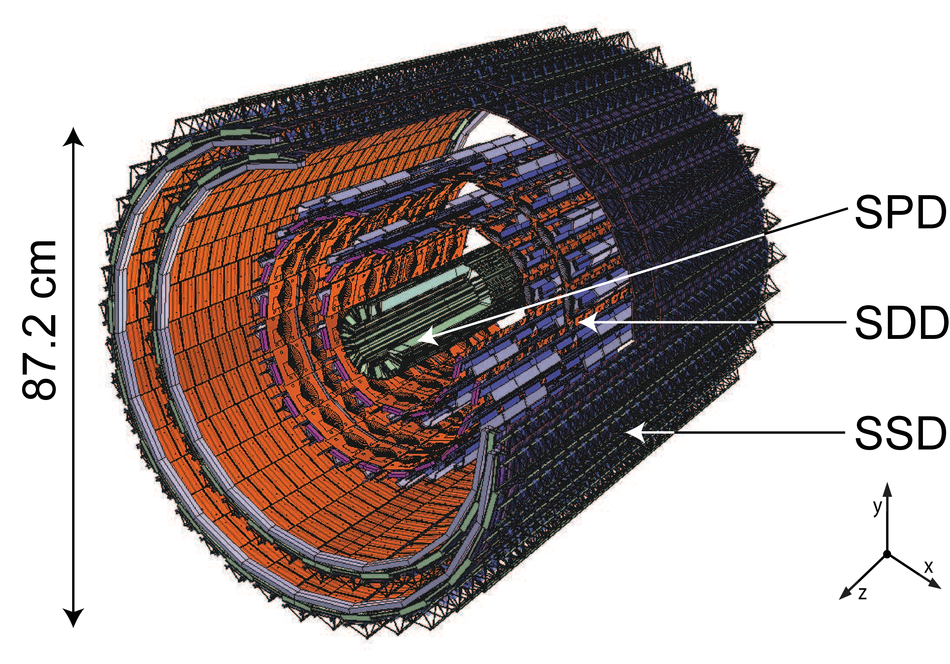
\includegraphics[width=0.7 \textwidth]{gfx/its}
	\caption{Layout of the ALICE Inner Tracking System, with three different subdetectors.}
	\label{fig:its}
\end{figure}

\paragraph{Silicon pixel detectors} 
SPD are the two innermost layers of the ITS and are
used for the determination of the primary vertex position as well as for the measurement of
the impact parameter of secondary tracks.
Furthermore, SPD, provides a quick trigger signal which contributes to the Level 0 trigger of 
the experiment.

\paragraph{Silicon drift detectors} 
SDD are the two intermediate layers of the ITS. The technology used for the SDD 
allows us to have high 2D resolution with limited number of read-out channels and to fulfil the
request of having a low material budget.

\paragraph{Silicon strip detectors}
SSD are the outer layers of the ITS and are equipped with double sided silicon detectors, which
provide a two dimensional measurement of the track position.
The information of the SSD is crucial for the matching of the tracks from ITS to TPC, being the
nearest layers to the TPC.

The main task of the ITS is the reconstruction of primary and secondary vertices, and the tracking
of the low \pt particles.
The first objective is achieved with a resolution better than 100 $\mu$m, while for the second the
ITS extends the tracking of the low \pt particles down to $\pt = 80 \; \mevc$, thanks to its high
spatial resolution (Table \ref{tab:its}) and low material budget.
The total material budget of the ITS, keeping into account also the support structures and the 
thermal shields, is 7.18 \% X/X0.
The SSD, together with the SDD, provide also the measurement of the energy loss of particles 
in their sensitive volume, extending the ALICE Particle IDentification (PID) capabilities in the
 \pt region below 200 \mevc.

\begingroup
\renewcommand{\arraystretch}{1.5} % Default value: 1
\begin{table}
\centering
\begin{tabular}{lccc}
\textbf{Parameter}                      &  \textbf{SPD} & \textbf{SDD}  & \textbf{SSD} \\
\midrule
Material budget per layer (\%$X_{0}$)   &  1.14 - 1.14  &  1.13 - 1.26  &  0.83 - 0.86 \\
Spatial resolution $r\phi$ ($\mu$m)     &       12      &       35      &       20     \\
Spatial resolution $z$ ($\mu$m)         &       100     &       25      &      830     \\
Two track resolution $r\phi$ ($\mu$m)   &       100     &      200      &      300     \\
Two track resolution $z$ ($\mu$m)       &       850     &      600      &     2400     \\
Active cell size ($\mu$m$^2$)           & 50$\times$425 & 202$\times$294& 95$\times$40000 \\
Number of readout channels (k)          &      9835     &      133      &     2603     \\
\midrule
\end{tabular}
\vspace{2pt}
\caption{Details about the material budget and spatial resolution of the ITS subdetectors \cite{alicemulti}. The material budget is reported for each single layer.}
\label{tab:its}
\end{table}
\endgroup

%
\subsection{Time Projection Chamber} \label{sec:tpc}

The Time Projection Chamber (TPC), illustrated in Figure \ref{fig:tpc}, is the main ALICE
tracking detector with good two-track separation. It is also one of the main PID detectors as it
provides the information about the specific energy loss of the particles in its volume in a large
momentum range. 

\begin{figure}
    \captionsetup{justification=centering}
    \centering
    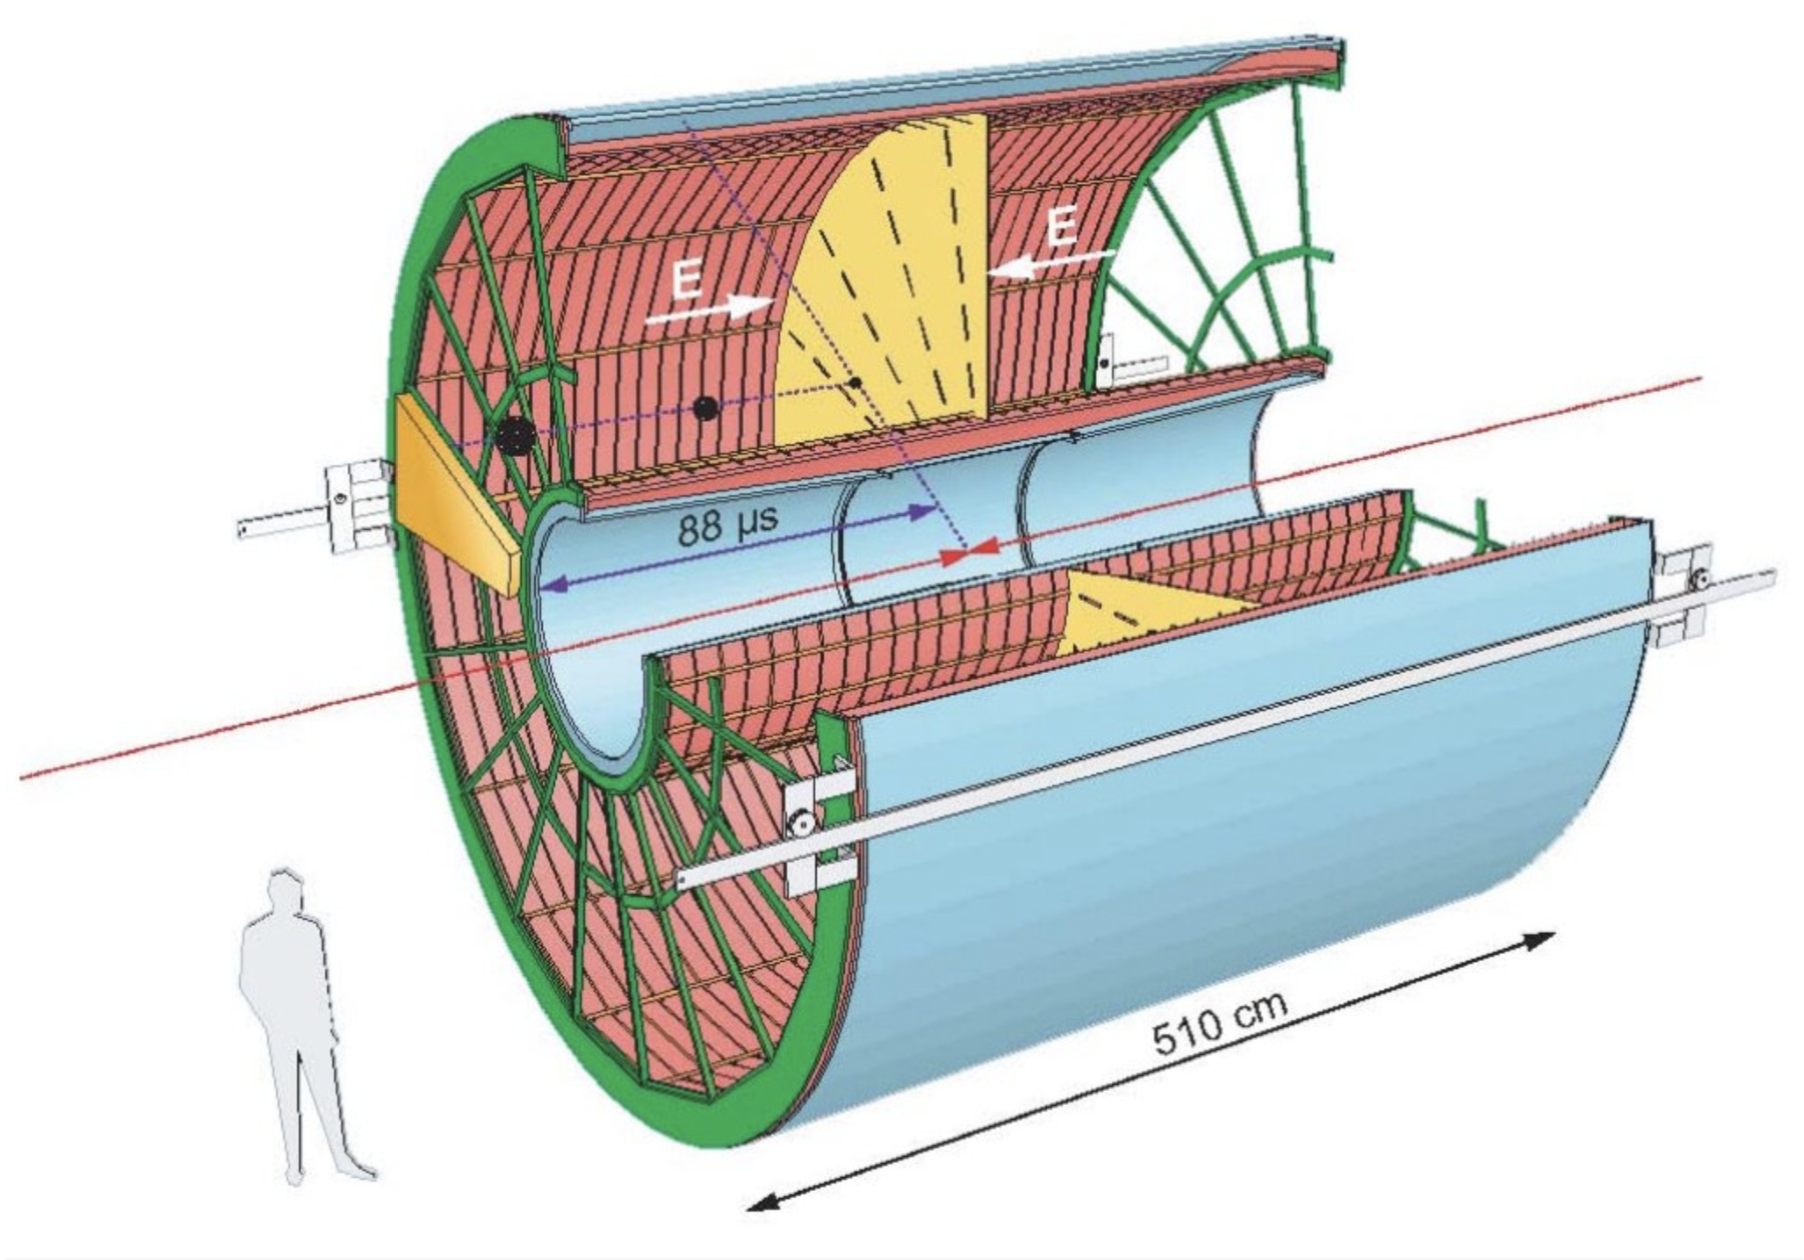
\includegraphics[width=0.8\textwidth]{gfx/tpc}
	\caption{Schematic layout of the ALICE Time Projection Chamber.}
	\label{fig:tpc}
\end{figure}

The TPC is a 88 m$^3$ cylinder filled with gas and divided in two drift regions by the
central electrode located at its axial centre. 
For the LHC Run 2 (2015-2018) the used gas is a mixture of Ar and CO$_2$.
The field cage secures the uniform electric field along the $z$ axis.
Charged particles travelling in the TPC gas ionise the gas along their path, liberating electrons 
that drift towards the end plates of the cylinder. 
Each end plate is equipped with 36 readout chambers, which are organized in 18 sectors, covering 
20$^{\circ}$ in azimuth each. 
The readout chambers consist in a system of multi-wire proportional chambers (MWPC) with cathode pad
read-out. Each sector is segmented by pads organized in rows and the longitudinal coordinate is given
by the drift time. 
Thanks to this segmentation, charged particles can be tracked and identified with up to 159 
3-dimensional space points (TPC clusters), including also the specific energy loss information
for the PID. The TPC radial position and acceptance are reported in Table \ref{tab:alice}.

%
\subsection{Time Of Flight detector} \label{sec:tof}

The Time of Flight detector (TOF) has a cylindrical geometry and consists of a large area array of 
Multi-gap Resistive-Plate Chambers (MRPC).
With a sensitive area of 7.4 × 120 cm$^2$ each and an intrinsic resolution of about $\sim\;$ 40 ps 
\cite{alicemulti}. TOF is used to identify charged particles and light nuclei in the momentum interval 
0.2--4 \gevc in the central pseudorapidity range ($|\eta|$ < 0.9).
The time of flight of a particle is determined by measuring the time between the event collision and the
particle TOF hit cluster. 
The time of flight of the particle together with the momentum, obtained from the track curvature, 
allows us to compute the particle $\beta$ and, as a consequence, its mass.
The precise determination of the event collision time, the so called $t_{0}$, represents an important
ingredient for the TOF PID and it is determined by using the information from the T0 detector as 
well as from the TOF. 

%
\subsection{T0 detector} \label{sec:t0}

The T0 detector consists of two arrays of Cherenkov counters placed on both sides of the interaction point 
along the $z$ axis (Table \ref{tab:alice}).
It is mainly used to determine the event collision time ($t_{0}$) with a resolution below 50 ps
and  independently from track and vertex reconstruction. 
The T0 information provides also the Level 0 trigger when the position of the vertex falls in
appropriate intervals.

%
\subsection{V0 detector} \label{sec:v0}

The V0 is a small angle detector consisting of two arrays (V0A and V0C) of 64 scintillators counters 
distributed in 8 rings and they are installed on both sides of the ALICE interaction point 
(Table \ref{tab:alice}). 
The V0 detectors are used to define the minimum bias (MB) trigger in ALICE and to determine the
centrality in p–Pb and Pb–Pb collisions.

%
%
\section{Trigger and Data Acquisition} \label{sec:data_flow}

The trigger system in ALICE is managed by the Central Trigger Processor (CTP) \cite{alice_trigger} 
which collects and synchronises all the trigger inputs coming from all the triggering detectors 
with the information on the LHC filling scheme providing a trigger signal to the readout detectors
in case of fulfilled trigger conditions. 
The Level 0 trigger (L0) decision is taken by using the fast detectors: SPD, V0, T0, EMCal, PHOS and 
muon trigger. The L0 signal arrives to the CTP in 1.2 $\mu$s after the collision happens. 
The signals from the detectors which are not fast enough for L0 trigger are collected in the level 1
(L1) trigger signal and sent to the CTP after 6.5 $\mu$s. 
Finally the third level trigger is sent after 88 $\mu$s, which is the maximum drift time of electrons
in the TPC, in order to maximize the rejection of the pile-up events in the TPC.
The minimum-bias (MB) trigger  selection in ALICE is defined by the logical "\textit{or}" between the
signals of V0A, V0C and SPD detectors. This minimum-bias trigger is the one used in the analysis
presented in this thesis.

The events passing all three trigger selections are then sent to both the Data Acquisition (DAQ) machines 
and to the High Level Trigger (HLT).


The data fulfilling all the trigger requirements, are sent to the Local Data Concentrators (LDCs)
through optical connections, the Detector Data Links (DDLs).
LDCs is a farm of computers which build \textit{subevents} from the event fragments they receive from
the front-end electronics and then sends \textit{subevents} to the Global Data Collectors (GDCs).
The GDC compose the full event including information from the HLT.
At the HLT level a fast reconstruction of the data -- including clusterisation and track reconstruction --
is performed, allowing further selections that are not possible in the hardware triggers.
When the event building in the GDC is completed, the data are buffered in a local disk pool waiting 
to be transferred to the CERN computing centre, where they will be registered on tape.

%
%
\section{ALICE offline framework} \label{sec:offline}

The offline analysis framework is fundamental for any High Energy Physics experiment.
The huge amount of data collected by detectors requires a proper infrastructure able to process and 
analyse the reconstructed events.
Beyond that, modern experiments need a large number of Monte Carlo (MC) simulations, for the development of
the detectors, for performance studies, and also as a basis for physics analyses.

The infrastructure realised at CERN in order to menage the LHC data flow is the Worldwide 
LHC Computing Grid (WLCG). The mission of that project is to provide global 
computing resources to store, distribute and analyse the $\sim$50-70 Petabytes of data expected for each
year of operations of the LHC experiments.

The ALICE collaboration uses the WLCG resources for running MC simulations, event reconstruction and physics
analyses. In the following section more details about this aspects of the ALICE operations will be 
provided.

%
\subsection{Monte Carlo simulations} \label{sec:montecarlo}

The first step of Monte-Carlo simulations is the event generation. 
The ALICE simulation tools include generators suited for the different collision systems available at the LHC: proton-proton (pp), proton-ion (pA) and heavy ion (AA) collisions.
The event generator gives the set of all stable and weakly decaying particles produced in the collision,
with their starting kinematic parameters. The strongly decaying particles -- as the \dst dibaryon studied
in this analysis -- are usually handled at the generator level.
Then, the generated kinematic parameters are propagated, using a transport framework, through the
experiment, whose geometry and material budget are precisely described in the ALICE software.

Three different transport codes are available in the simulation framework: GEANT3, GEANT4 and FLUKA.
These tools provide the information on the behaviour of the transported particles through the sensitive
part of the detector, giving the particle energy loss. 
This information converted in detectors electronics signal through the simulation of each detector
response. Finally, the digitalised signal is stored in the same detector raw data format used in the 
real data taking and reconstruction.

%
\subsection{Event Reconstruction} \label{sec:event_rec}

The ALICE event reconstruction flow starts from the raw data, collected or simulated, and is 
schematically shown in Figure \ref{fig:rec_flow}. 

In the first step of the event reconstruction the detector raw data are converted into clusters, 
through a set of algorithms which perform the reconstruction for each detector separately.
All clusters are characterized by positions, signal amplitude and time.
Other information, like the energy lost by the particle, the time of flight or the Cherenkov 
angle are attached to the clusters in the PID detectors allowing the identification of the 
tracked particle.

The second step of the reconstruction is a preliminary estimation of the position of the primary
vertex using clusters in the SPD, the closest detectors to the interaction point.
The first estimate of the primary vertex is fundamental to speed-up the tracking algorithm searching
good candidate tracks, even if the final estimation of the position of the interaction vertex
needs the full track information.

Subsequently, the Kalman filter technique \cite{kalman} is used for performing track finding and
fitting in TPC and ITS. 
The main tracking detector, in ALICE, is the Time Projection Chamber. Therefore track are reconstructed 
starting from the TPC, then they are prolonged in the ITS looking for matches with the ITS 
reconstructed tracks. 
The found tracks are backward propagated searching, also, for a possible match in the other central
barrel detectors.
Finally, the primary vertex can be determined using the fully reconstructed tracks.

The last step of the event reconstruction chain is the search for photon conversion and decays of
strange hadrons.

\begin{figure}
    \captionsetup{justification=centering}
    \centering
    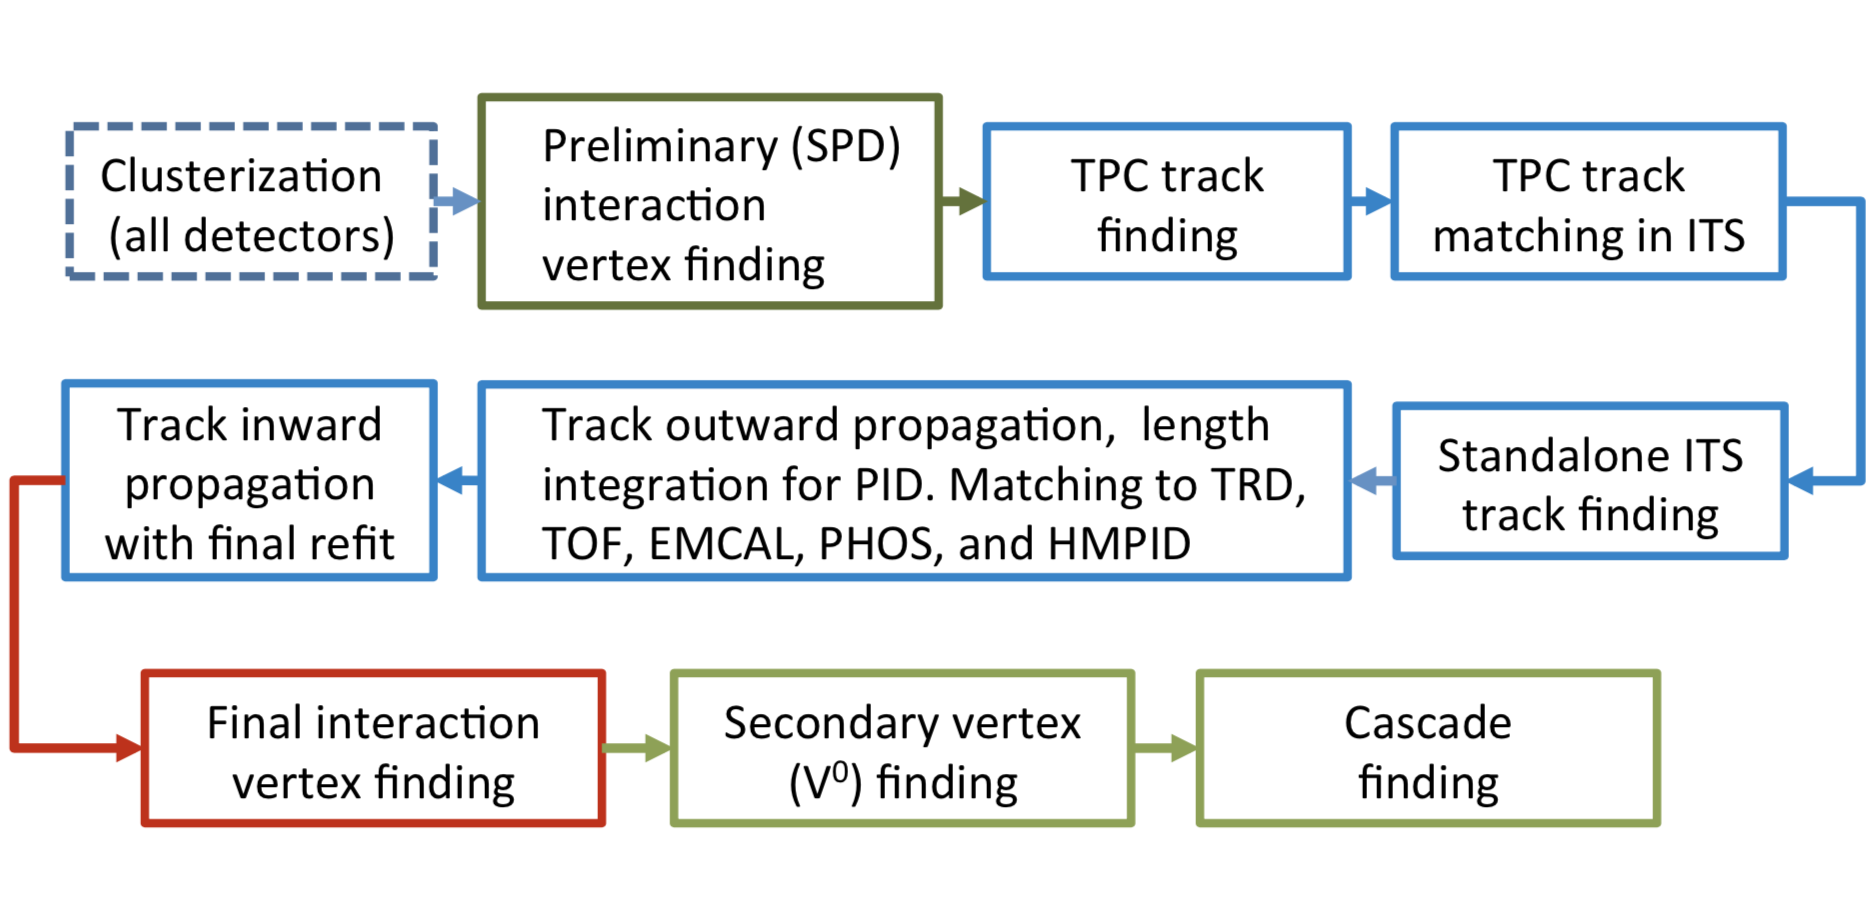
\includegraphics[width=0.9\textwidth]{gfx/reconstruction}
	\caption{Vertex and tracks reconstruction procedure in ALICE \cite{alice:Perf2014}.}
	\label{fig:rec_flow}
\end{figure}

%
\subsection{ALICE analysis framework} \label{sec:anal_frame}

The ALICE software infrastructure, that allows the access to the collected and simulated data 
available everywhere on the grid, is the Alien (ALICE Environment) \cite{alien} grid middleware.
Through the Alien user interface it is possible to launch the analysis tasks singularly on ALICE data. 
When more users are interested in analyzing the same data sample, is possible to use an optimized
access pattern, called \textit{analysis train}, which allows to run together all the tasks
of those users in the same jobs.
It defines a standard analysis flow in the ALICE experiment and it ensures the reproducibility of the
analyses.

The data collected by the ALICE experiment are stored in binary files using the ROOT framework data 
format.
The ALICE software environment is \textit{AliRoot}, introduce in 1998 and based on the ROOT framework
\cite{root}.
The analysis related code -- containing all the software used in physics analysis -- is collected
in a part of the ALICE offline framework denominated \textit{AliPhysics}.
The reconstructed events are stored in two different formats: the Event Summary Data (ESD) format, 
that is mainly used for calibration and detector performance studies, and the Analysis Object Data 
(AOD) format, which contains only the relevant information at the analysis level.

%
%
\section{ALICE performances} \label{sec:ali_perf}

The ALICE experiment was specifically designed for the demanding experimental environment of the 
\PbPb collisions. 
One of the most challenging task, in this conditions, is the precise reconstruction of both momentum
and origin of the particles produced.
In this section the tracking and vertexing performances of the ALICE experiment will be presented,
as well as the methods used for the particle identification.

%
\subsection{Tracking} \label{sec:tarcking}

The importance of the tracking process lies in its relation with the particle momentum
measurement and with the vertexing (Section: \ref{sec:vertexing}).

The momentum of a charged particle travelling in magnetic field is related to the radius of curvature
of the particle track. Therefore, measuring the radius of curvature, it is possible to measure the
particle momentum.
In particular, in colliders experiments, the interaction point is surrounded by cylindrical 
position-sensitive detectors located in magnetic field -- usually parallel to the beam axis -- 
which provide a measurement of the \textit{sagitta} of the track.
The particle momentum is related to the sagitta by the following expression:
\begin{equation}
    p = \frac{L^{2} q B}{8\,s},
\end{equation}
where $L$ is the lever arm length of the tracking detectors, $q$ is the charge of the particle and $B$
the magnetic field.
Therefore, the resolution on the particle momentum does not depend only on the magnetic field used,
but also on $L$ and, of course, on the resolution on the sagitta $\sigma_{s}$:
\begin{equation}
    \frac{\sigma_{p}}{p} \propto p \frac{\sigma_{s}}{B\,L^{2}}.
\end{equation}
Thanks to the large radial coverage ($0.039 \leq r \leq 3.680\ $ m), despite the mild solenoidal
magnetic field, the ALICE apparatus is able to reconstruct tracks over a wide momentum range.

The first stage of the tracking algorithm starts building the track seeds at a large radius of 
the TPC.
The seeds are propagated inward looking for other TPC cluster compatible with the track.
Whenever a compatible cluster is found the track parameters are updated using a Kalman filter 
\cite{kalman}. 
Different seeds can reuse the same cluster, therefore it is not uncommon to have two or more
tracks sharing some clusters. 
If the fraction of shared clusters is above a predefined threshold (between 25\% and 50\%), a
dedicated algorithm rejects the candidate tracks with the worst parameters quality.
The tracks with at least 20 clusters (out of a maximum of 159) and that miss no more than 50\% 
of the expected clusters are accepted and propagated to the inner radius of the TPC.
Figure \ref{fig:reconstruction} shows the track reconstruction efficiency in the TPC.

\begin{figure}
    \centering
    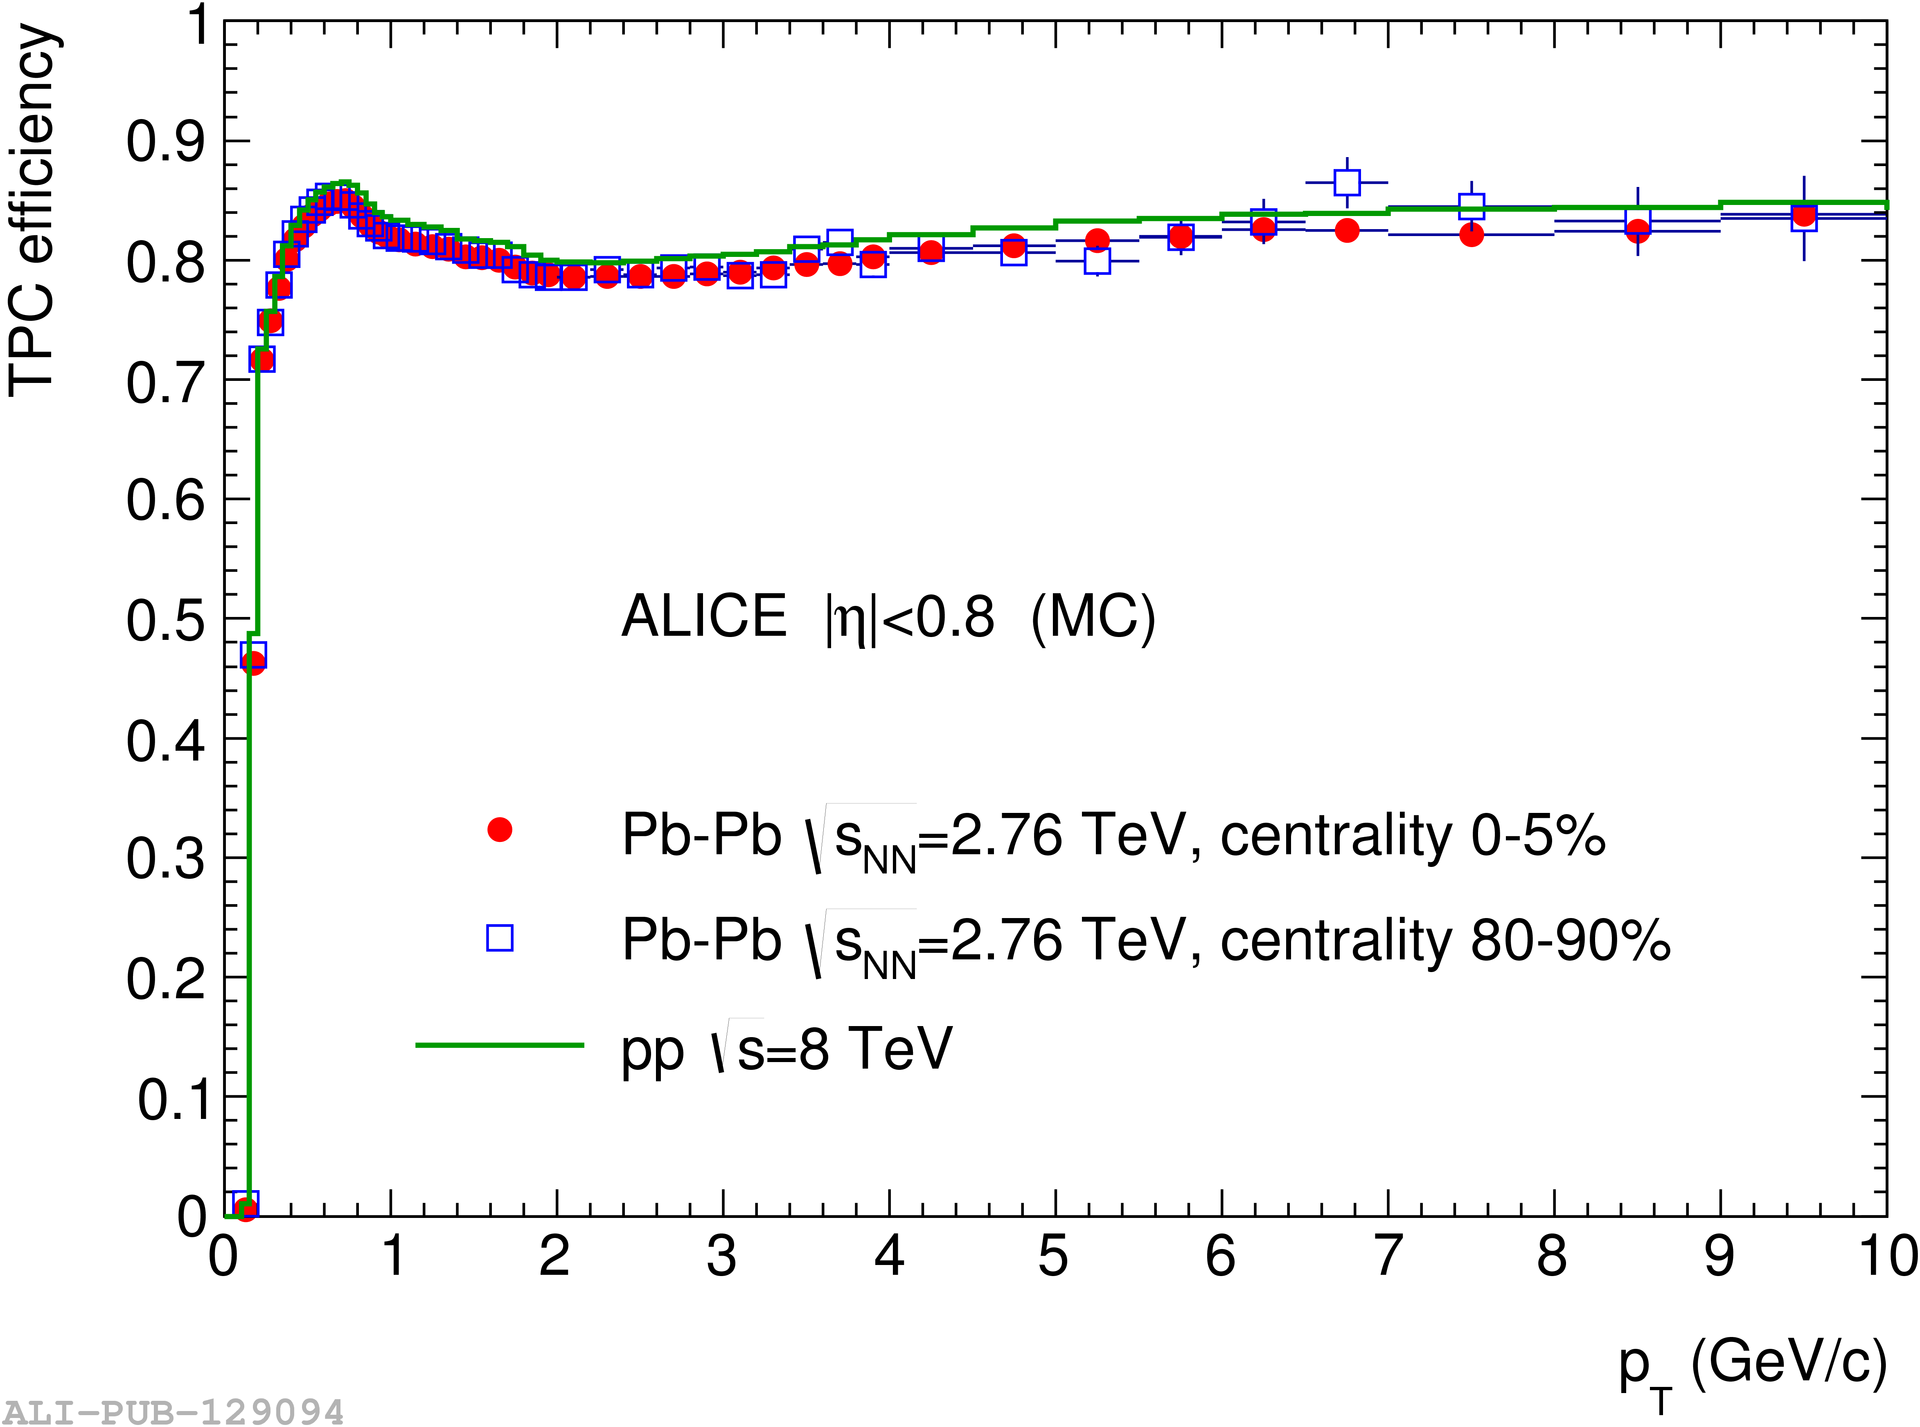
\includegraphics[width=0.7\textwidth]{gfx/tpc_rec_eff}
	\caption{TPC track reconstruction efficiency in pp (green line) collisions at \sotev and for central (red dots) and peripheral (blue open square) \PbPb collisions at \sdtev. The drop for $\pt \leq 0.5\; \gevc$ is due to energy loss in the detector material and the shape at higher \pt is related to the loss of clusters in the dead zones of the TPC. The efficiency does not depend on the detector occupancy.}
	\label{fig:reconstruction}
\end{figure}

The reconstructed TPC tracks are propagated to the SSD, the outermost layer of the ITS.
At this point, the tracking algorithm in ITS proceeds with a procedure similar to that adopted
for the TPC. 
Starting from the second layer of SSD, the seeds are propagated inward, penalizing tracks
for which a compatible cluster in the extrapolation is not found.
Among the prolongation candidates of the TPC track is selected the one with the highest quality.
This track is stored in the reconstructed event as ITS+TPC track.

The second stage of the tracking algorithm is the backward refit of the ITS+TPC tracks using the
Kalman filter.
The track is backward propagated looking for matching with TRD tracklets. If the matching is
successful, updates the track parameters using the TRD tracklet information. 
During this process, at each step, the integrated track length and the expected time of flight
for different particle species are computed and the related track parameters are updated.
This information is used for a correct particle identification in the Time Of Flight detector
(Section: \ref{sec:PID}).
Then an attempt to extrapolate the track and match it to one of the TOF clusters is performed.
The track length integration and time of flight calculation are stopped at this stage.
Finally a further extrapolation is performed to match the track with other external central
barrel detectors as HMPID, PHOS and EMCal.

The final stage of the track reconstruction, consists in propagating all the tracks from the TRD
back to the innermost ITS layer. 
In each detector (TRD, TPC and ITS) the tracks are refitted using the information of all attached
clusters.
If the refit process goes well the track \textit{refit flag} is switched on.
At this stage the track’s position, direction, inverse curvature and its associate covariance 
matrix are determined.

\begin{figure}
    \centering
    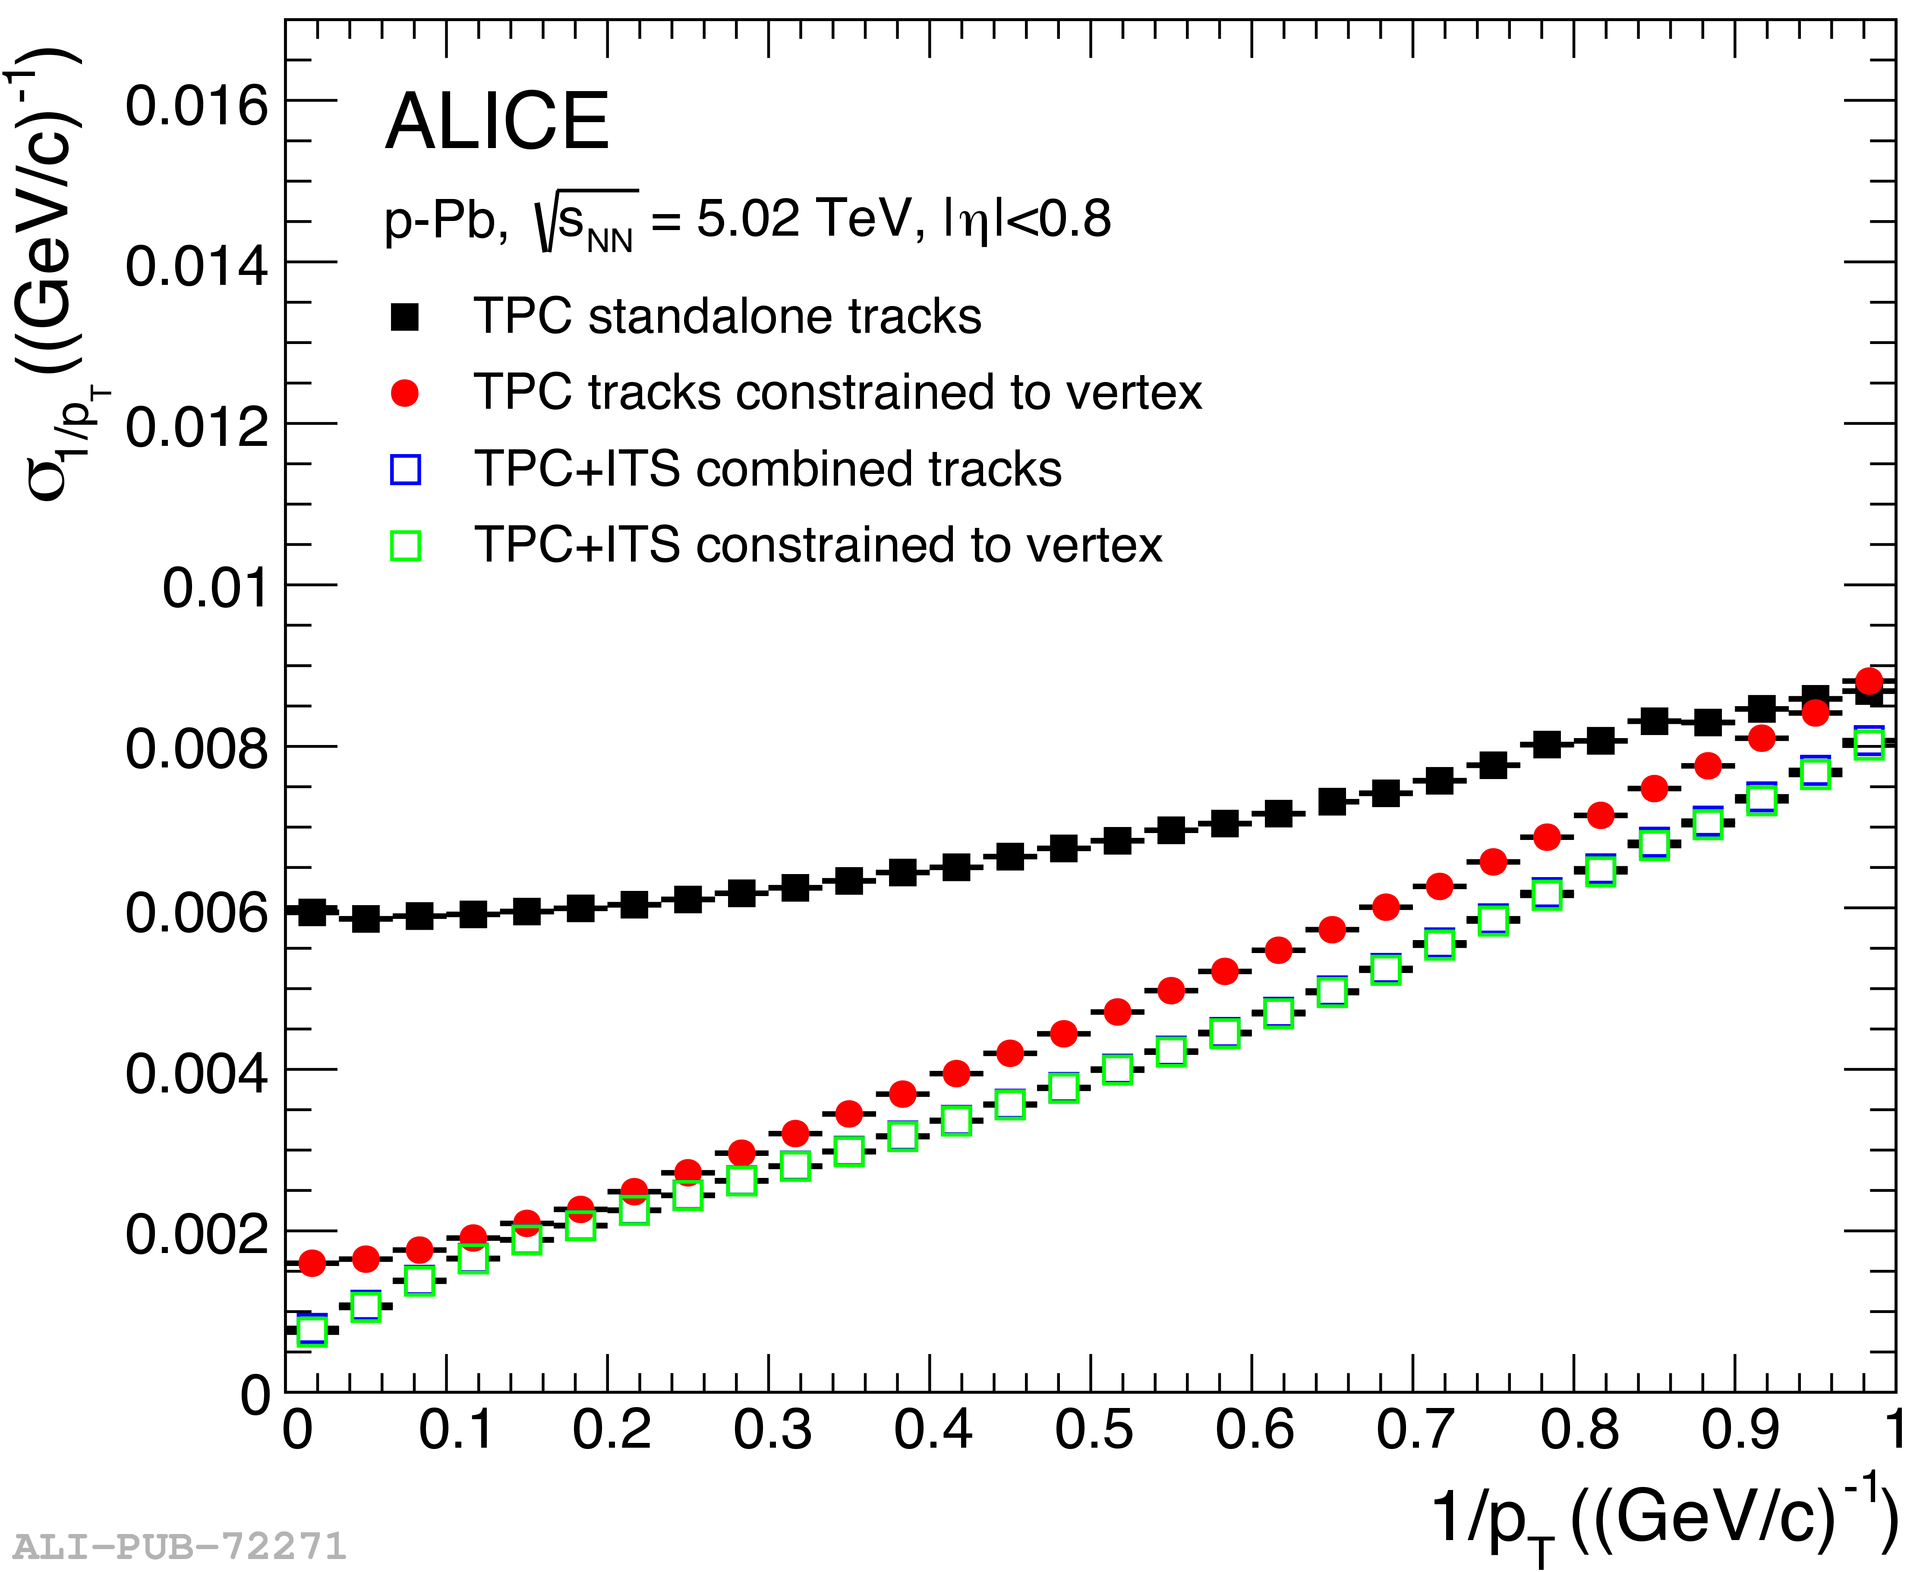
\includegraphics[width=0.6\textwidth]{gfx/ptresolution}
	\caption{Resolution on the 1/\pt parameter as a function of 1/\pt in \pPb collisions. The resolution is quoted for TPC tracks with (red dots) and without (black squares) vertex constraint and for ITS+TPC tracks with (green square) and without (blue square) vertex constraint. The resolution is quoted for 1/\pt because this can be extracted directly from the covariance matrix of the Kalman Filter fit.}
	\label{fig:vertres}
\end{figure}

Following the described process the ALICE apparatus can reconstruct track with resolution
between 1\% and 10\% in the momentum range from 0.1 to 100 \gevc. 
Figure \ref{fig:vertres} shows the 1/\pt resolution for standalone TPC and ITS+TPC tracks which
is related to the \pt resolution by the formula:
\begin{equation}
    \frac{\sigma_{\pt}}{\pt} = \frac{\sigma_{1/\pt}}{1/\pt}.
\end{equation}
The effect of constraining the tracks to the primary vertex is shown as well and considering,
for instance, TPC standalone tracks the resolution is reduced from 6\% to 2\% at low \pt by 
this requirements.

%
\subsection{Vertexing} \label{sec:vertexing}

\subsubsection{Primary vertex reconstruction}
A first estimation of the interaction vertex is obtained by using the clusters on the two layers of 
SPD. The algorithm matches the clusters on the SPD layers inside a fixed azimuthal window,
building a set of segments, called tracklets.
Then the space point which minimise the distance from all the tracklets is computed and represents
the interaction vertex estimation.
At least two tracklets are required for a 3D reconstruction of the primary vertex position.
This estimation is very fast, but the most precise determination of the primary vertex position is 
obtained by using the full reconstructed track information (Figure \ref{fig:vertres}).
The full reconstructed tracks, obtained at the end of the tracking procedure, are propagated to the
nominal beam line and the tracks too far from it are excluded from the vertex computation.

\begin{figure}
    \centering
    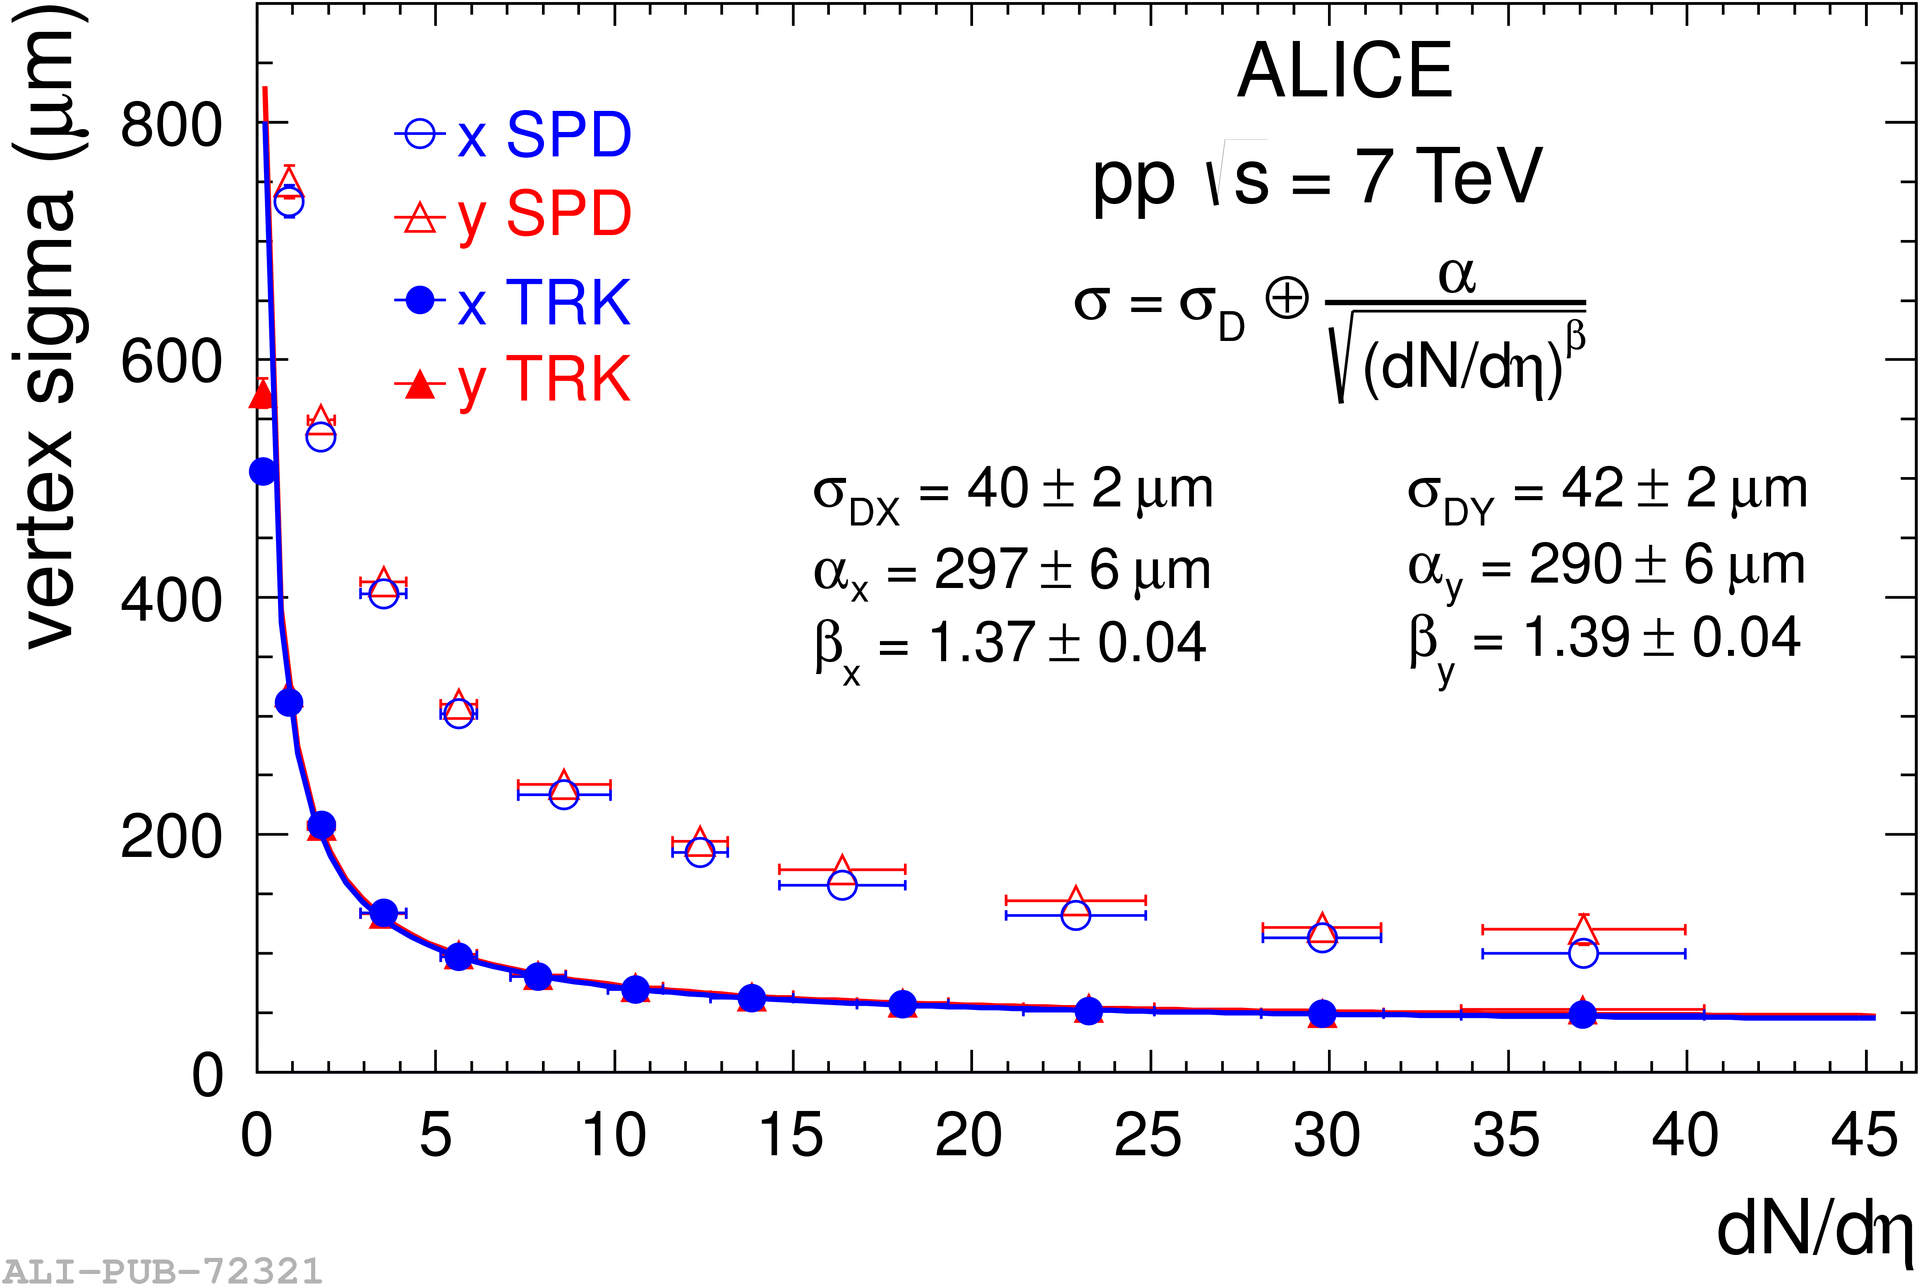
\includegraphics[width=0.7\textwidth]{gfx/vertexres}
	\caption{Resolution on the primary vertex position using the SPD clusters (open markers) and the full track informations (full markers) as a function of the charged particle multiplicity of the event in pp collisions at  \cite{alicemulti}.}
	\label{fig:vertres}
\end{figure}

\subsubsection{Secondary vertex reconstruction}
Once the tracks and the primary vertex have been reconstructed, the event reconstruction procedure
searches for secondary vertices from particle decays.
The reconstruction of the secondary vertexes from decays of neutral particles and with a V-shaped track 
topology of the daughters is performed with the $V^{0}$ finder algorithm.
The basic principle of the $V^{0}$ finder algorithm is the matching of two tracks with opposite sign,
which are close in the space and presumably come from the decay of one mother particle.
The combined tracks and the resulting mother momentum are requested to pass quality selection criteria
before being tagged as $V^{0}$ candidate.
The $V^{0}$ finder algorithm is implemented in the ALICE software and performed with two different
procedures, the offline and the on-the-fly.

In the reconstruction process the Distance of Closest Approach (DCA) -- the minimum 
distance of the track from the reconstructed vertex -- is computed for all the reconstructed
track in the beam line direction (DCA$_{z}$) and in the transverse plane (DCA$_{xy}$).
This two parameters are stored together with the track.
In the offline analysis these parameters are used to reject tracks that don't come from the 
primary vertex.

%
\subsection{Particle Identification} \label{sec:PID}

One of the main feature of the ALICE experiment is the Particle Identification capability with high
resolution. To achieve this performances the information provided by different detectors are combined.
For the charged hadron identification the ITS, the TPC, the TOF and the HMPID are used.
The ITS and the TPC provide information on the specific energy loss of the tracked charged particles.
The TOF detector measures the time of flight and the HMPID, a ring-imaging Cerenkov detector,
measuring the Cerenkov angle, gives the $\beta = v / c\ $ of the particle.
Those detectors can be used all together but, most common, the particle identification is performed
combining the information provided by just few detector.
The choice of which detector to use in a particular analysis is dictated by the subject of the analysis.

\subsubsection{TPC particle identification} \label{sec:TPC_PID}

\begin{figure} 
    \centering
    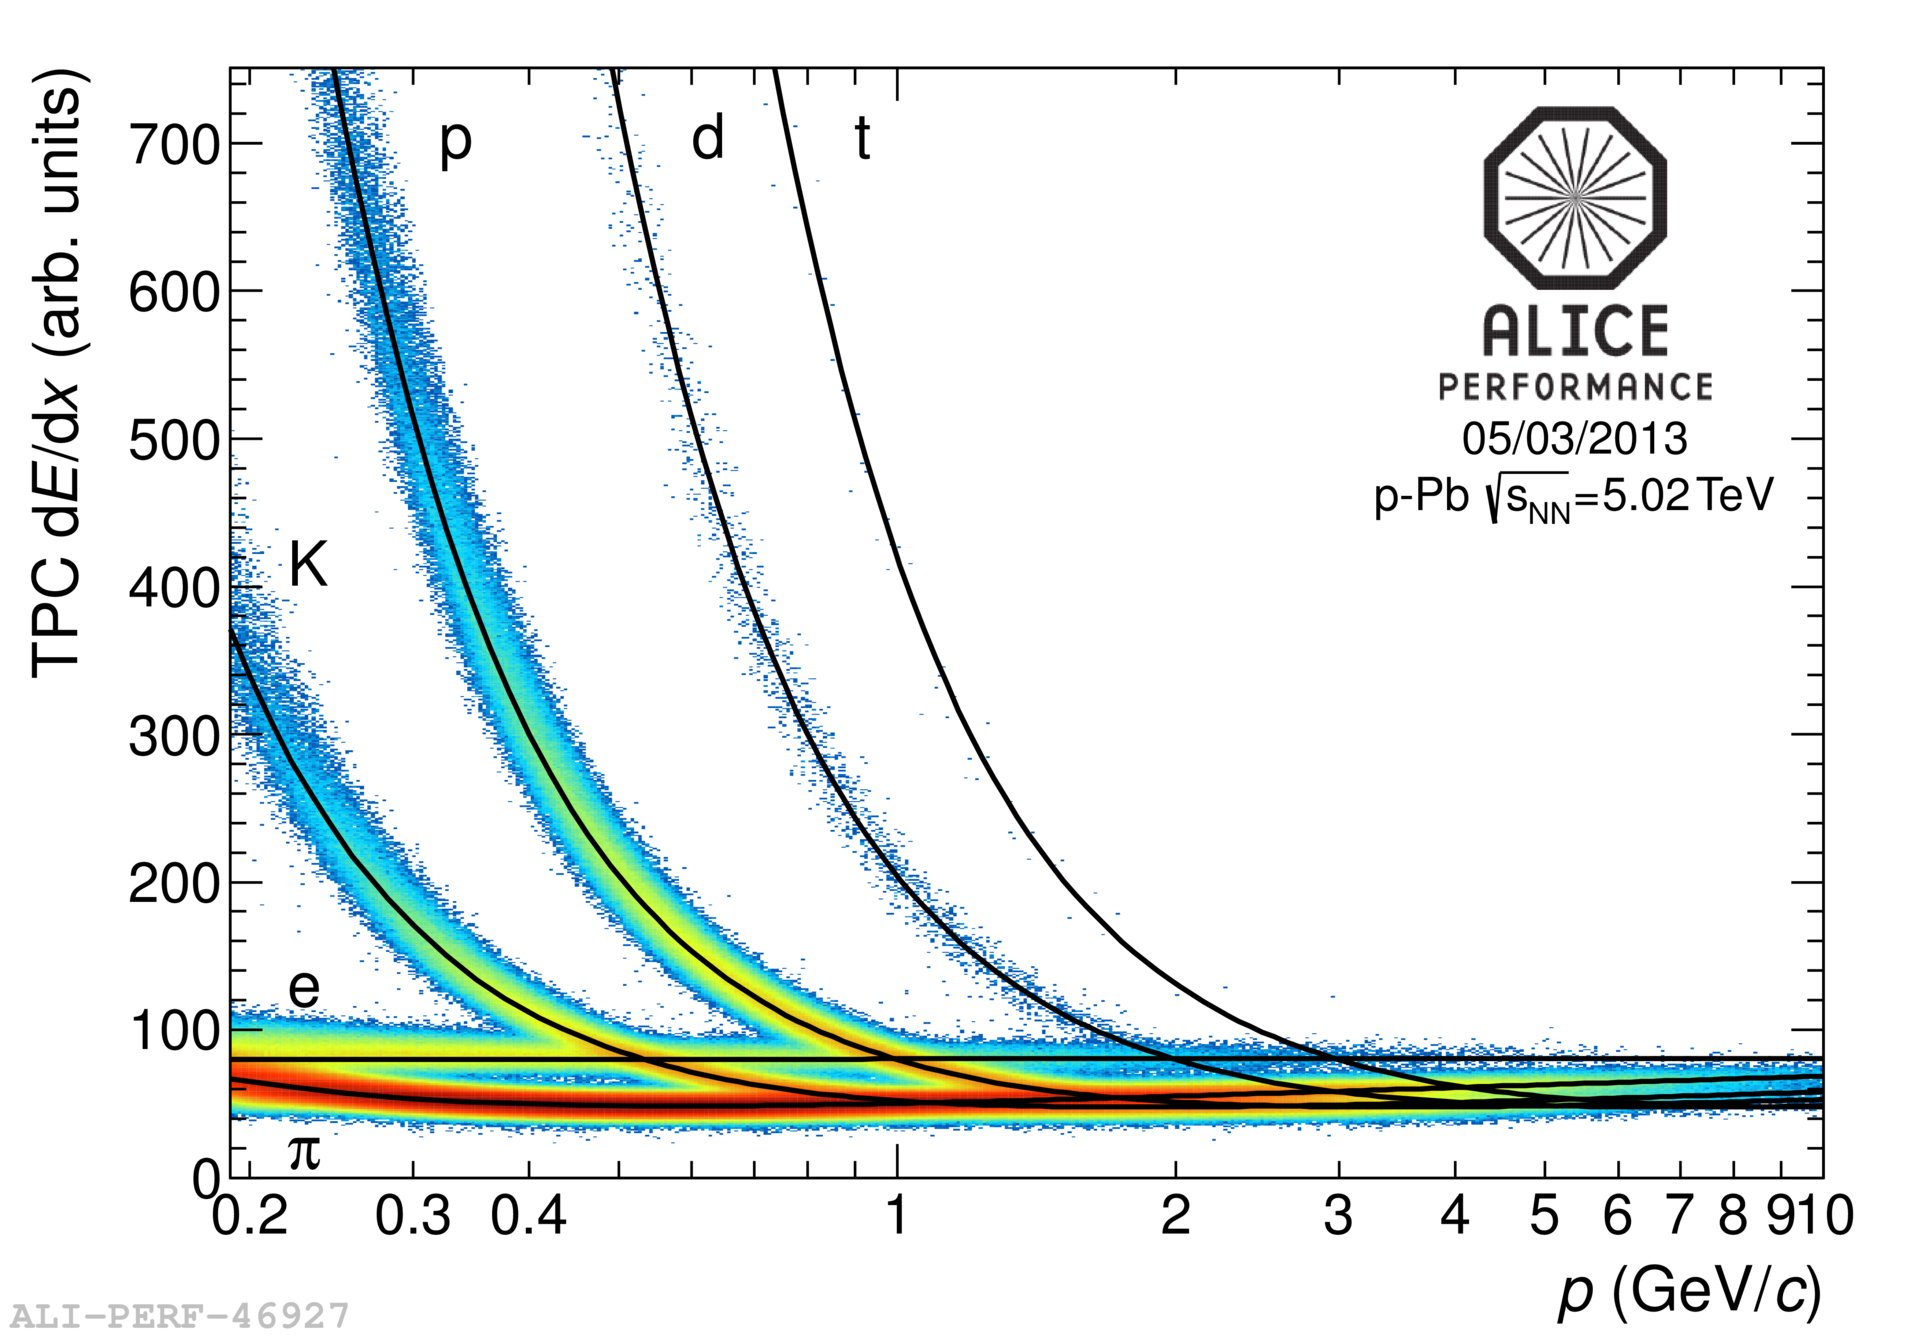
\includegraphics[width=0.75\textwidth]{gfx/pid_tpc_gen}
	\caption{Specific energy loss as a function of the rigidity for particles traversing the TPC gas in \pPb collisions at \sctev. The black lines represent the expected detector response for different particles.}
	\label{fig:pid_tpc}
\end{figure}

In the TPC particles are identified by measuring their specific energy loss in the detector gas.
Up to 159 padrows measure the charge generated in the gas by the passing particle in the ionisation
process. This charge is related to the particle energy loss by the value of the detector electric
field and by gain factors linked to the detector features. 
The resulting \dedx is obtained as the truncated mean of the single padrow measurement.

Particle identification is performed by measuring simultaneously the specific energy loss \dedx 
and the momentum of each particle traversing the detector gas.
The energy loss as a function of the momentum in TPC has been parametrised with a function originally
proposed by the ALEPH collaboration \cite{aleph}:
\begin{equation} \label{eq:aleph}
    f(\beta \gamma) = \frac{P_{1}}{\beta^{P_{4}}} \left( P_{2} - \beta^{P_{4}}
    - \ln \left( P_{3} + \frac{1}{(\beta \gamma)^{P_{5}}} \right) \right),
\end{equation} 
where $\beta$ is the particle velocity, $\gamma$ is the Lorentz factor and $P_{1-5}$ are the fit
parameters, obtained from a fit to the experimental data.
Alternatively the response functions have been parametrised using splines as shown in Figure
\ref{fig:pid_tpc} which are provided by the ALICE analysis framework.

Finally, particles are identified following the $n\sigma$ method.
This method consists in selecting a fiducial band around the expected signal for the particle of
interest.
For each track, the distance from the expected signal is computed in terms of 
number of $\sigma$, where $\sigma$ is the signal resolution obtained with a Gaussian fit to the 
signal distribution at each momentum interval:
\begin{equation} \label{eq:nsigma}
    n\sigma = \frac{S_{measured} - S^{i}_{expected}}{\sigma^{i}_{expected}}.
\end{equation}
In Eq. ~\ref{eq:nsigma} $S_{measured}$ is the measured signal for the candidate track,
$S^{i}_{expected}$ is the expected signal for the species $i$ and $\sigma^{i}_{expected}$ is the
expected detector resolution for the same species $i$.

In the specific case of the TPC particle identification $S^{i}_{expected}$ represents the
expected specific energy loss for the species $i$ \ -- given by the equation \ref{eq:aleph}
or by the splines -- \ while $S_{measured}$ is the measured \dedx.

The \dedx resolution is about 5.2\% in pp collisions and 6\% in \PbPb collisions.
A clear identification of the particle species, with the TPC, is possible up to $p \sim 1 \gevc$,
since at higher momenta the specific energy loss of different particle species are superimposed.

\begin{figure} [!h]
    \centering
    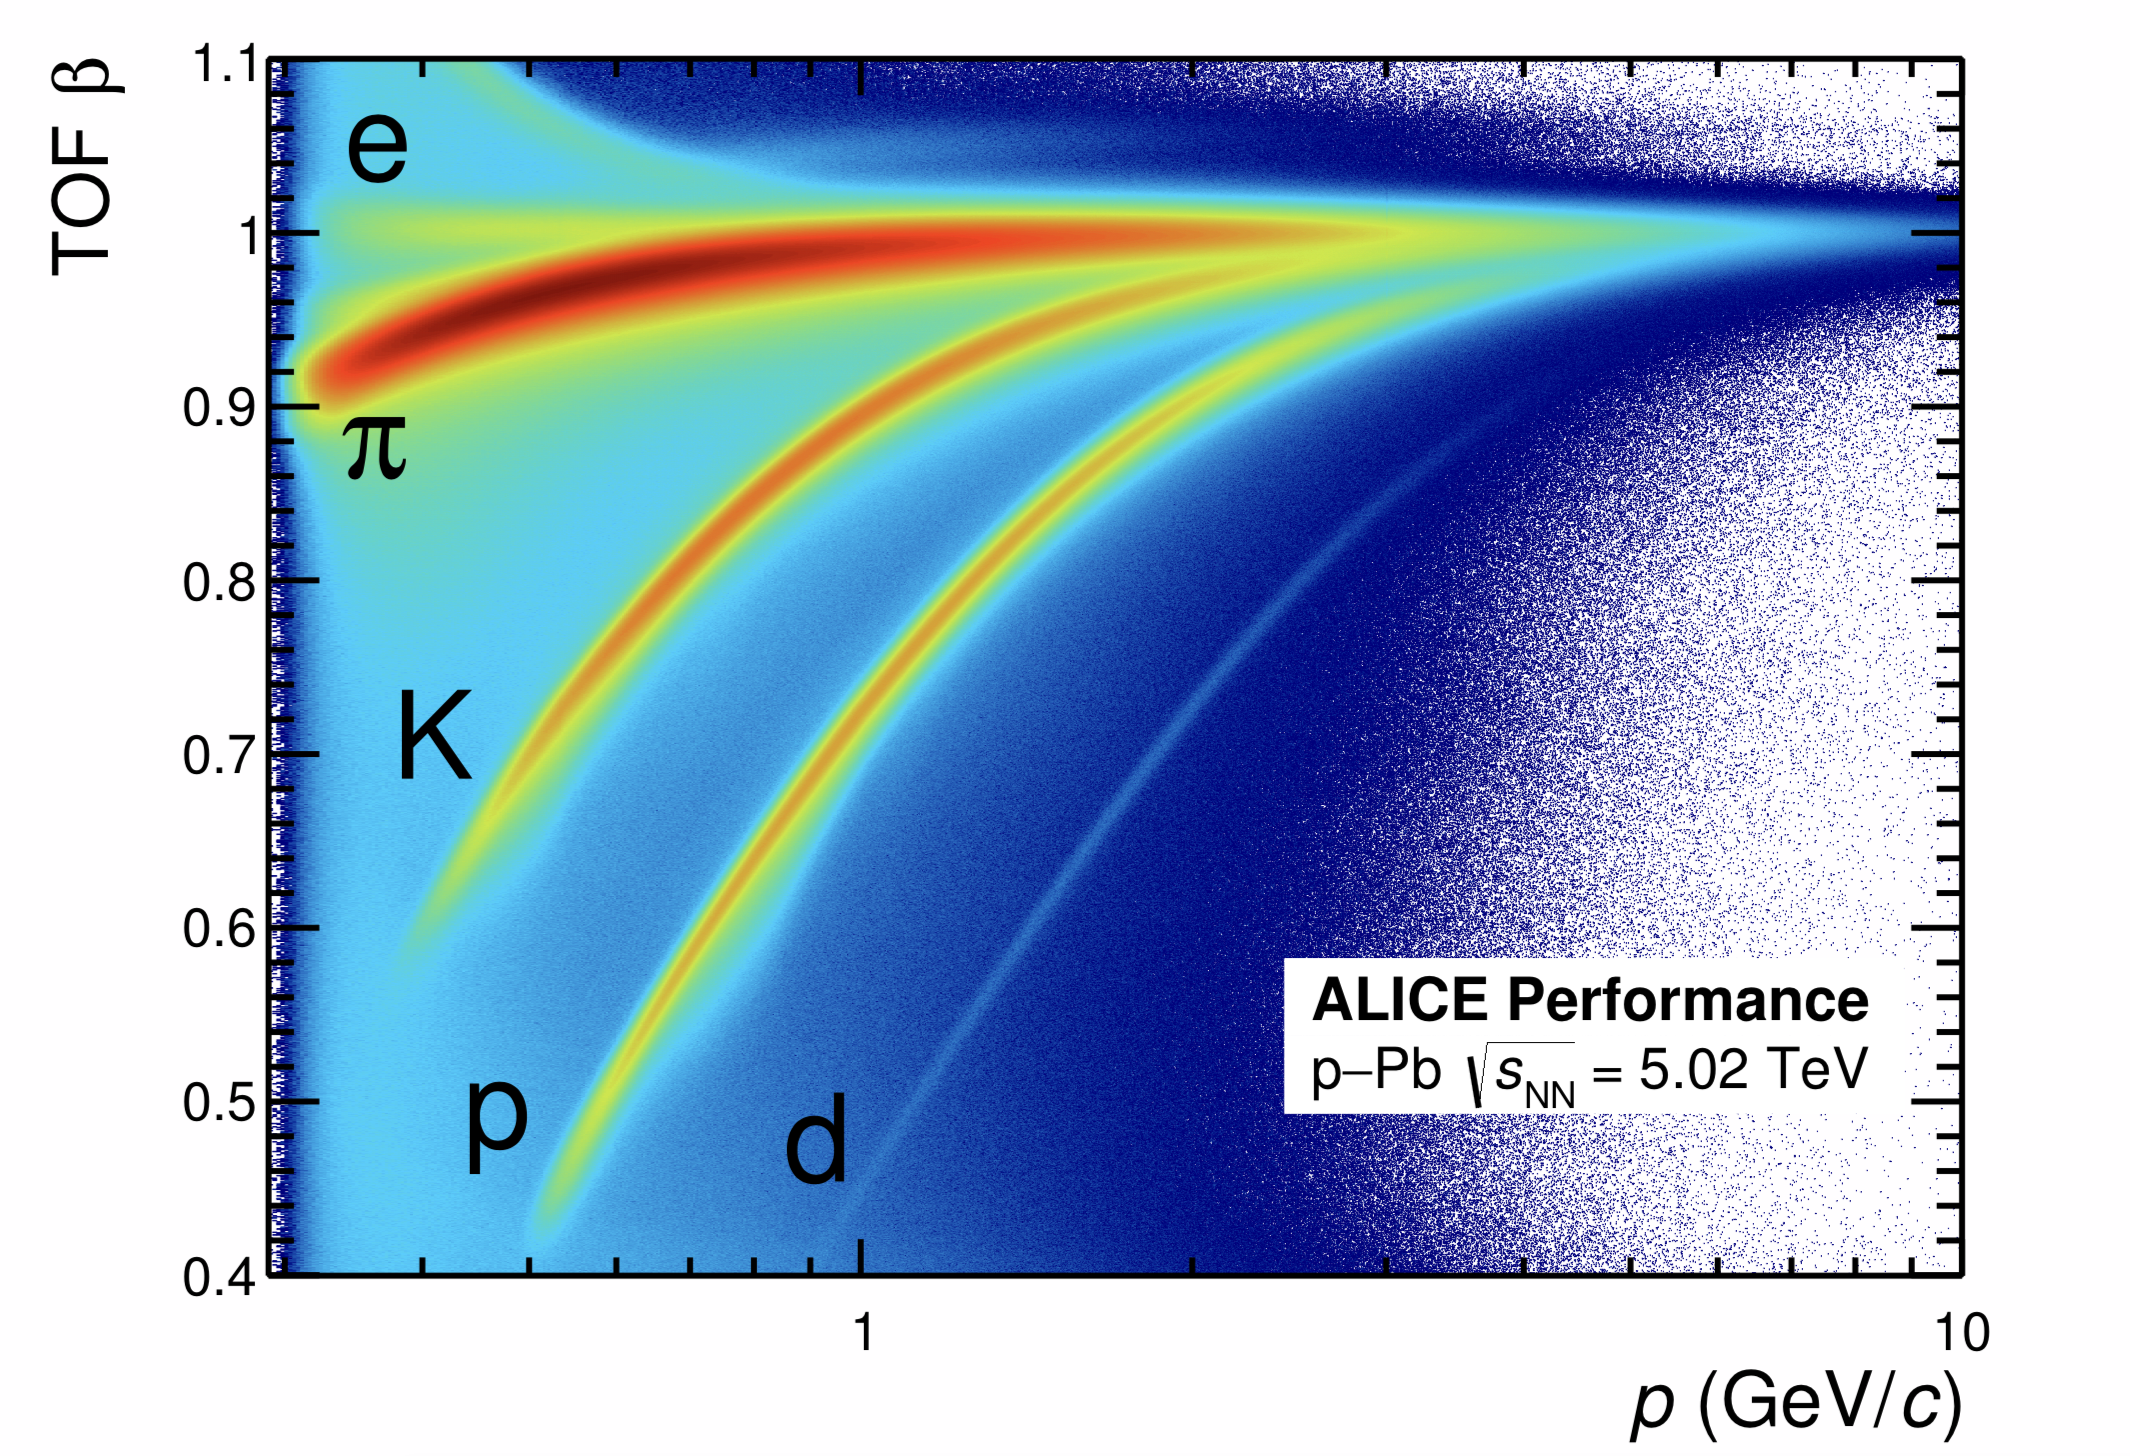
\includegraphics[width=0.75\textwidth]{gfx/pid_tof}
	\caption{$\beta$ of the particles in \pPb events at \sctev computed using the time of flight information from the TOF detector as a function of the measured track momentum.}
	\label{fig:pid_tof}
\end{figure}

\subsubsection{TOF particle identification} 

The TOF detector, described in section \ref{sec:tof}, determine the mass of a particle measuring 
the time of flight.
Using the measured time of flight $t_{TOF}$ and the integrated track length $L$, determined in the 
tracking process it is possible to compute the particle $\beta$ with the classical formula:
\begin{equation}
    \beta\,c = \frac{t_{TOF}}{L}.
\end{equation}
Figure \ref{fig:pid_tof} shows the measured particle $\beta$ as a function of the momentum estimated
in the tracking procedure.
It is also visible the mismatch background, which is due to tracks incorrectly matched to TOF
clusters. This background is an effect related to the TOF occupancy.

The particle identification with TOF detector follows the $n\sigma$ method described in the 
previous section (Sec. ~\ref{sec:TPC_PID}). In the specific case of the TOF, the measured and the 
expected signal are represented by the measured and the expected time of flight of a specific
particle specie.

Thanks to its excellent time resolution the TOF detector provides the information for PID in the
intermediate momentum range, up to 2.5 \gevc for pions and kaons, 4 \gevc for protons and 5 \gevc
for deuterons.


% \begin{figure}
% \begin{subfigure}{.5\textwidth}
%   \centering
%   \captionsetup{justification=centering}
%   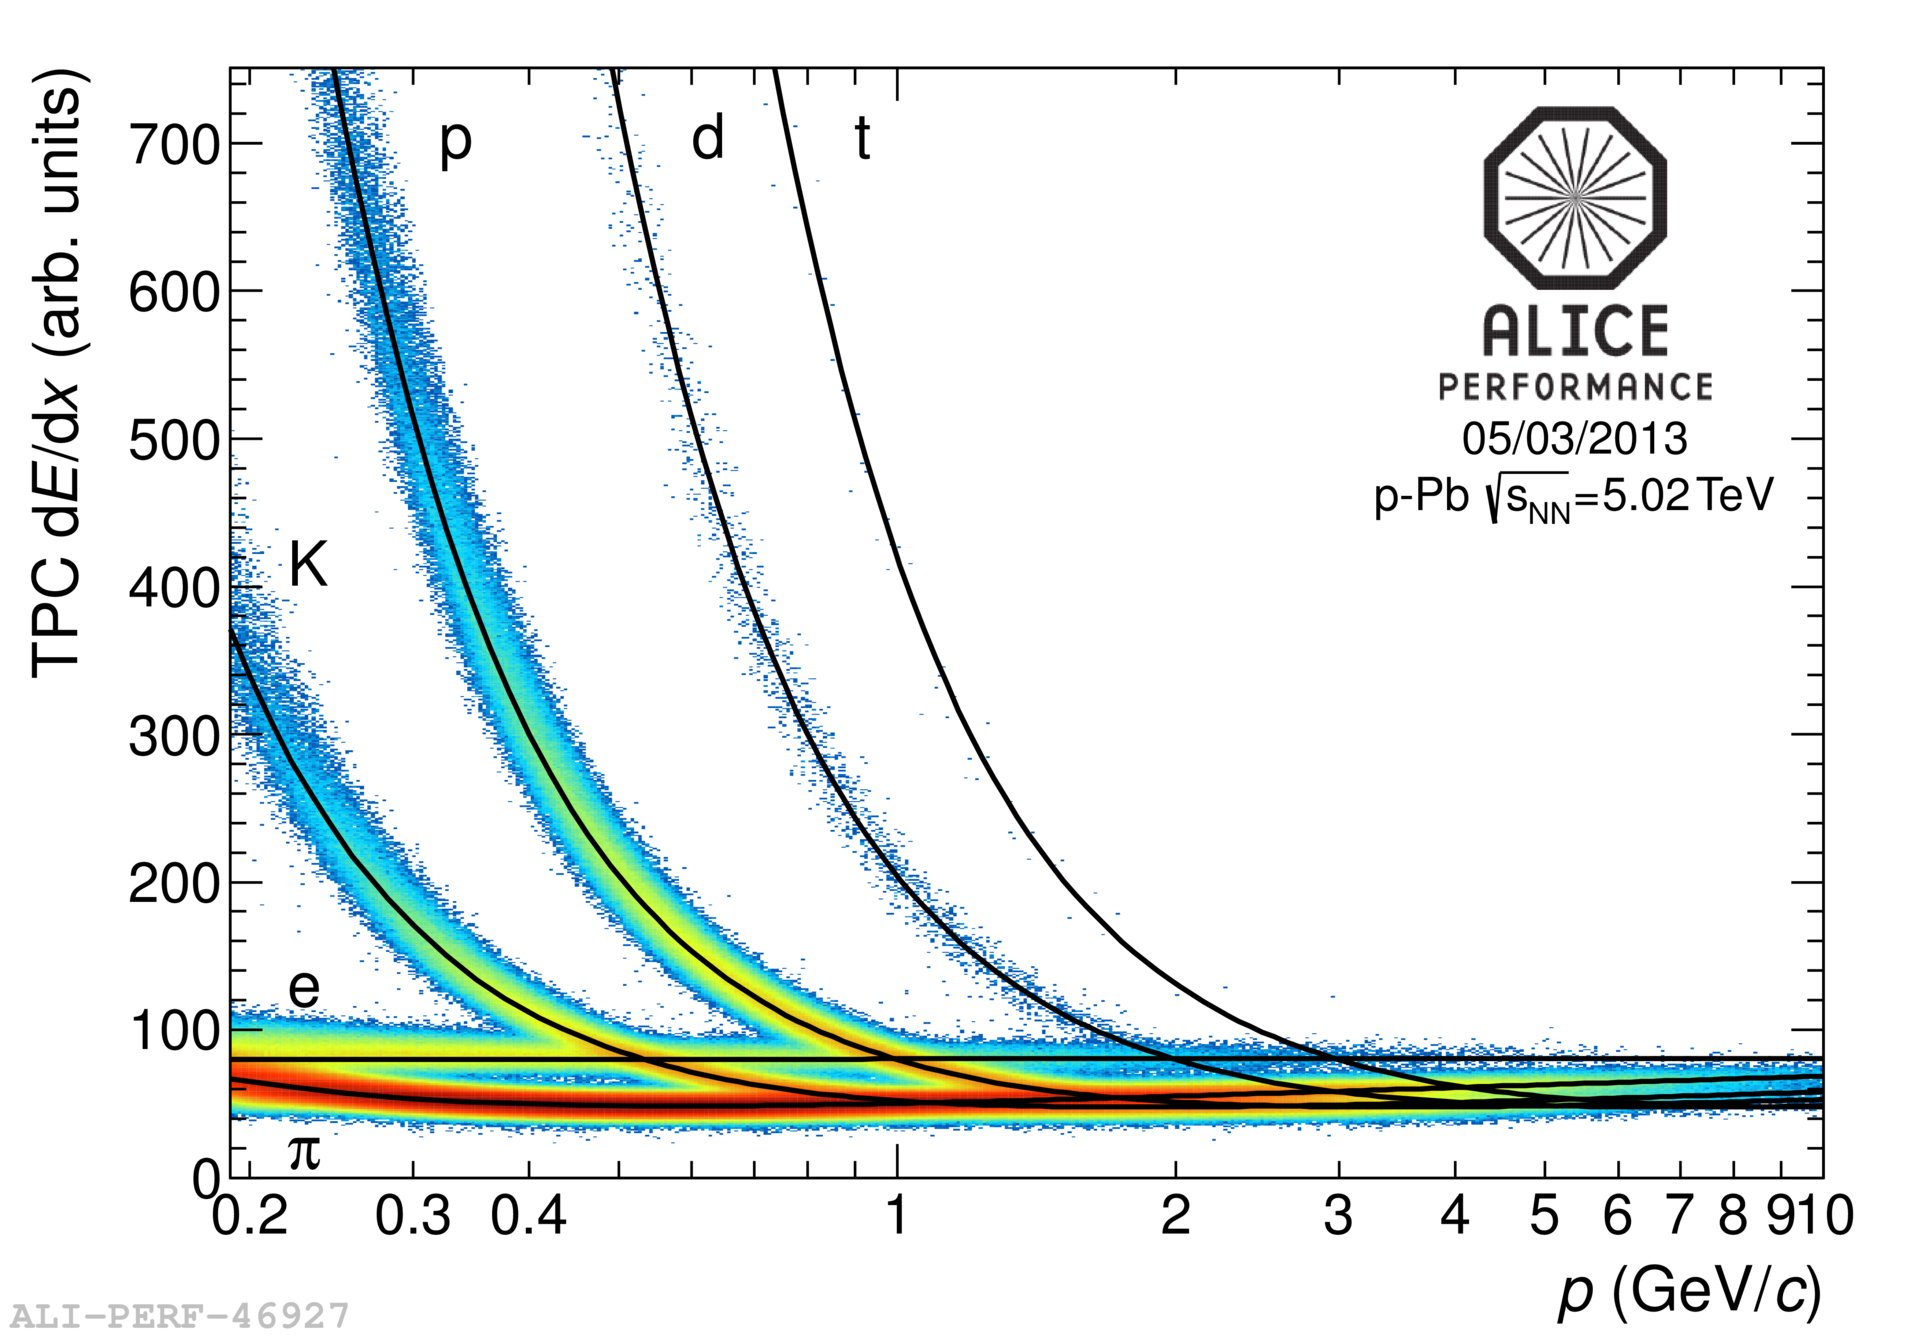
\includegraphics[width=\linewidth]{gfx/pid_tpc_gen}
%   \caption{}
%   \label{fig:pid_tpc}
% \end{subfigure}%
% \begin{subfigure}{.5\textwidth}
%   \centering
%   \captionsetup{justification=centering}
%   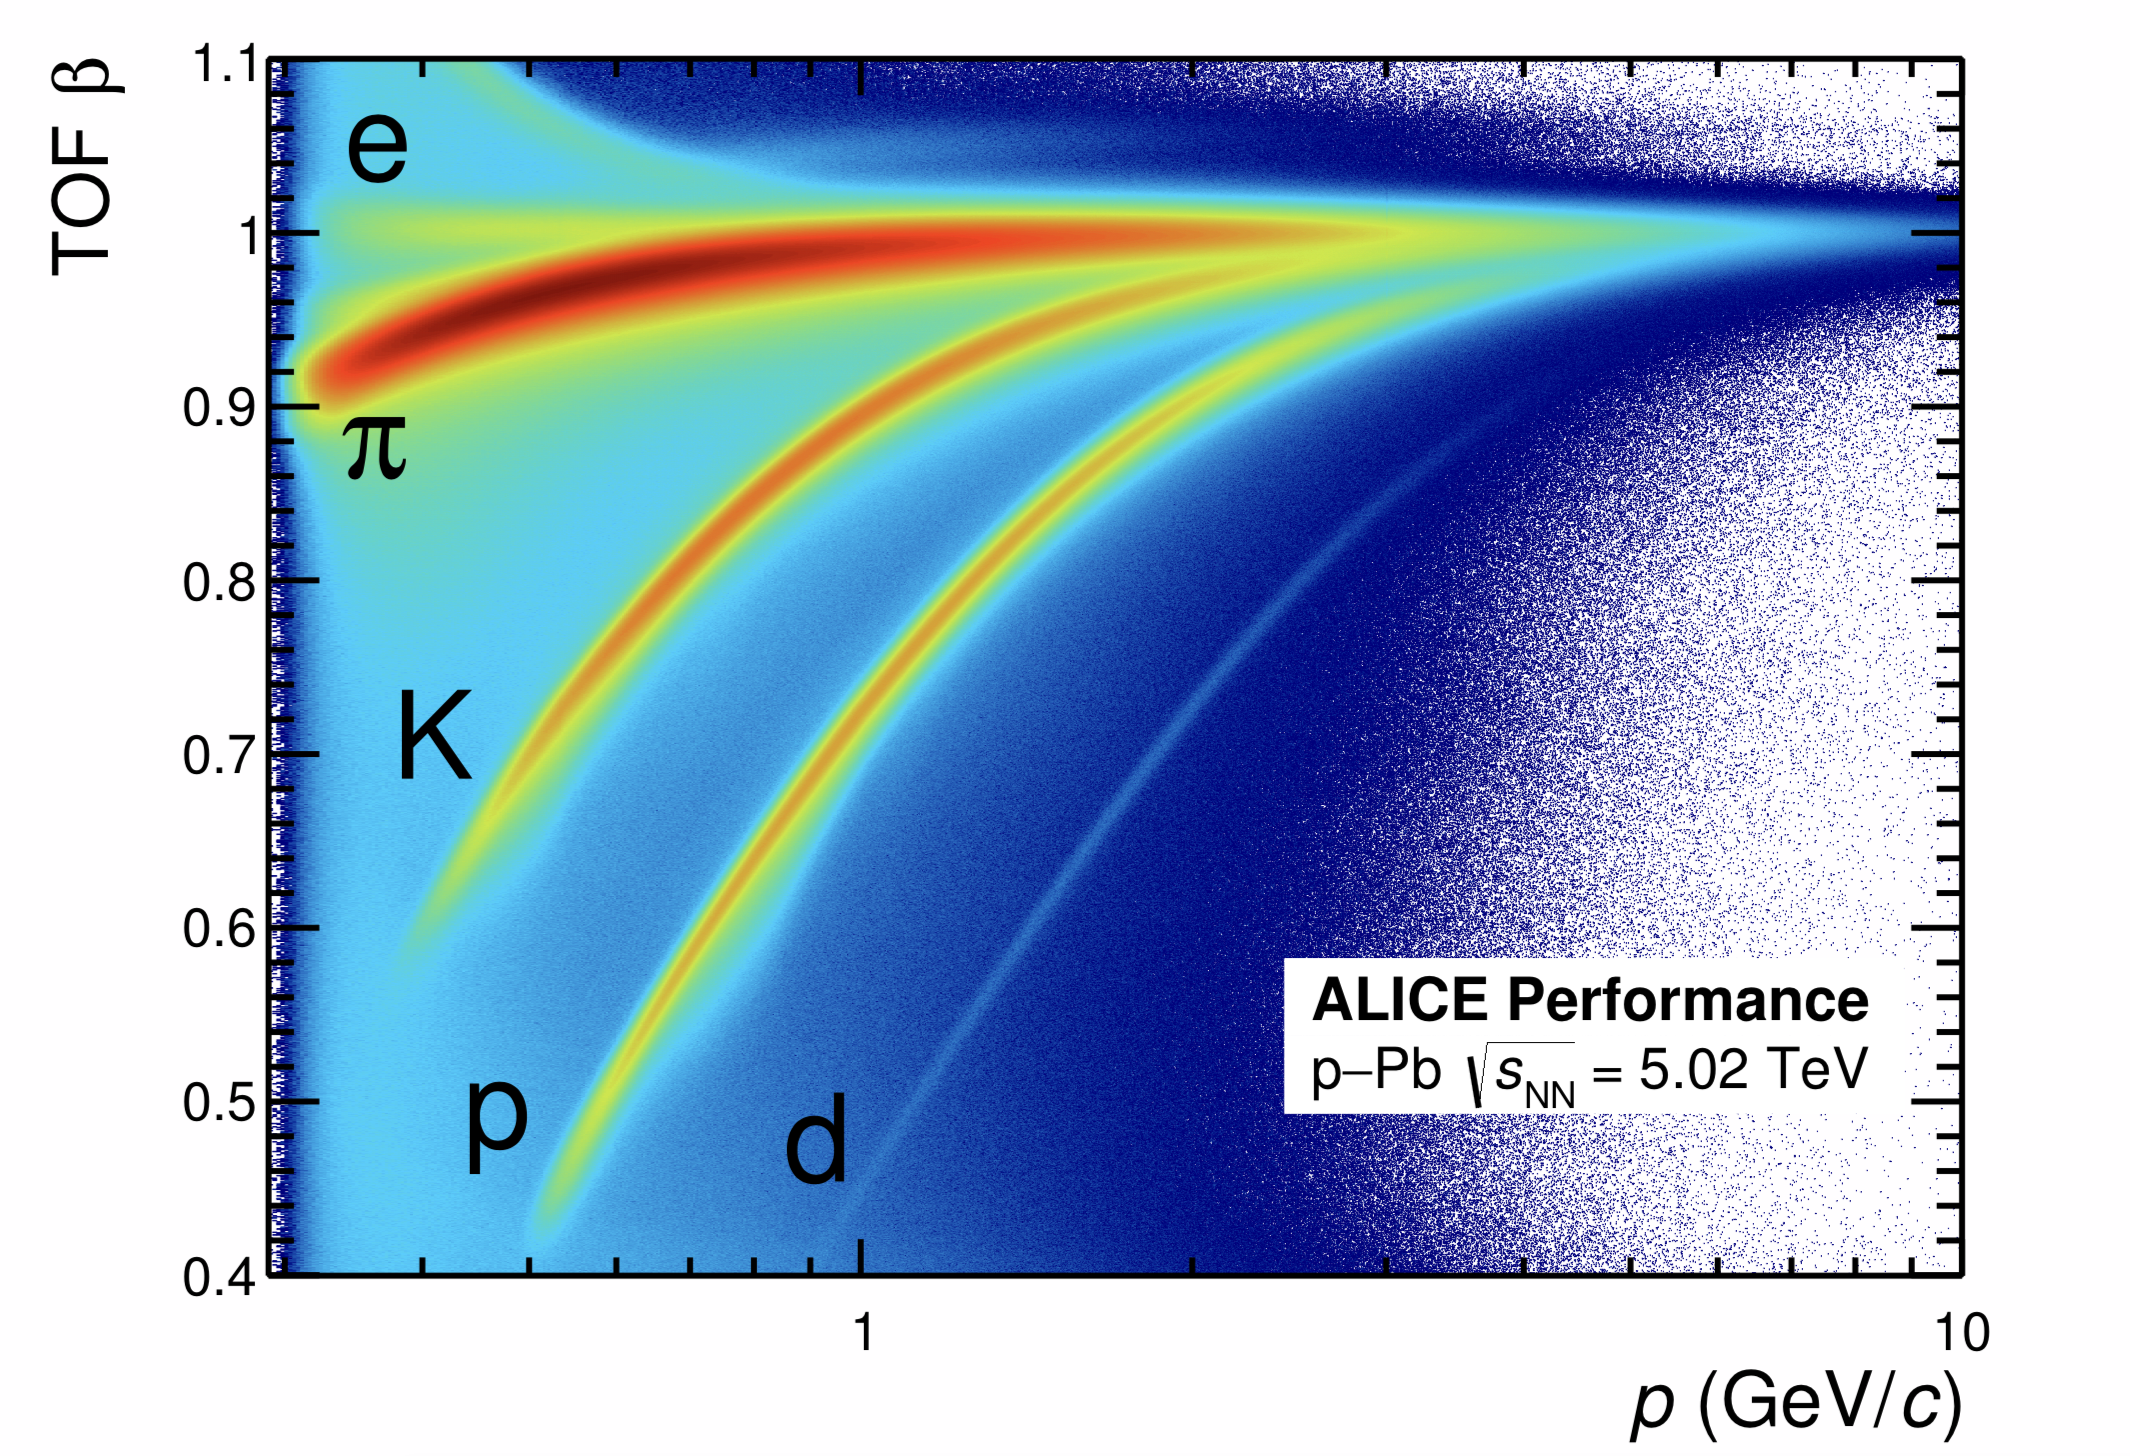
\includegraphics[width=\linewidth]{gfx/pid_tof}
%   \caption{}
%   \label{fig:pid_tof}
% \end{subfigure}
% \caption{Panel (a): specific energy loss as a function of the rigidity for particles traversing the TPC gas in \pPb collisions at \sctev. The black lines represent the expected detector response for different particles. Panel (b): measured $\beta$ of the particles in \pPb collisions at \sctev as a function of the track momentum.}
% \label{fig:pid_per}
% \end{figure}
 		% INCLUDE: ALICE chapter
\cleardoublepage

% --------------------------
% Back matter
% --------------------------
{%
\setstretch{1.1}
\renewcommand{\bibfont}{\normalfont\small}
\setlength{\bibitemsep}{0.5\baselineskip plus 0.5\baselineskip}
\printbibliography
% \printbibliography[heading=subbibliography,title={Webseiten},type=online,prefixnumbers={@}]
}
\cleardoublepage

% \listoffigures
\cleardoublepage

% \listoftables
\cleardoublepage

% **************************************************
% End of Document CONTENT
% **************************************************
\end{document}